\documentclass[10pt,twocolumn,letterpaper]{article}

\usepackage{cvpr}
\usepackage{times}
\usepackage{epsfig}
\usepackage{graphicx}
\usepackage{amsmath}
\usepackage{amssymb}
\usepackage{multirow}
\usepackage{color}
\usepackage{array}
\usepackage{subcaption}
\newcolumntype{L}[1]{>{\raggedright\let\newline\\\arraybackslash\hspace{0pt}}m{#1}}
\newcolumntype{C}[1]{>{\centering\let\newline\\\arraybackslash\hspace{0pt}}m{#1}}
\newcolumntype{R}[1]{>{\raggedleft\let\newline\\\arraybackslash\hspace{0pt}}m{#1}}
\usepackage{mathtools}
%\usepackage[demo]{graphicx}


\makeatletter
\renewcommand\paragraph{\@startsection{paragraph}{4}{\z@}%
           {1.25ex \@plus1ex \@minus.2ex}%
           {-1em}%
           {\normalfont\normalsize\bfseries}}
            
\renewcommand\subsubsection{\@startsection{subsubsection}{3}{\z@}%
                {-2ex\@plus -1ex \@minus -.2ex}%
                {0.1ex \@plus .2ex}%
                {\normalfont\normalsize\bfseries}}
                
                
% Include other packages here, before hyperref.

% If you comment hyperref and then uncomment it, you should delete
% egpaper.aux before re-running latex.  (Or just hit 'q' on the first latex
% run, let it finish, and you should be clear).
\usepackage[pagebackref=true,breaklinks=true,letterpaper=true,colorlinks,bookmarks=false]{hyperref}

\cvprfinalcopy % *** Uncomment this line for the final submission

\def\cvprPaperID{1798} % *** Enter the CVPR Paper ID here
\def\httilde{\mbox{\tt\raisebox{-.5ex}{\symbol{126}}}}

% Pages are numbered in submission mode, and unnumbered in camera-ready
\ifcvprfinal\pagestyle{empty}\fi
\begin{document}

%%%%%%%%% TITLE
%\title{Creating Album Highlights Automatically}
\title{Event-specific Image Importance\\(Supplementary Material)}



\author{First Author\\
Institution1\\
Institution1 address\\
{\tt\small firstauthor@i1.org}
% For a paper whose authors are all at the same institution,
% omit the following lines up until the closing ``}''.
% Additional authors and addresses can be added with ``\and'',
% just like the second author.
% To save space, use either the email address or home page, not both
\and
Second Author\\
Institution2\\
First line of institution2 address\\
{\tt\small secondauthor@i2.org}
}

\maketitle
%\thispagestyle{empty}

%%%%%%%%% BODY TEXT
\section{Dataset}
In the main paper, we calculated Kendall's $W$ of the image rating from 5 workers from Amazon Mechanical Turk (AMT) in order to measure the consistency among people's rating. We further tested the statistical significance of Kendall's $W$. As shown in the main paper, there are different percentages of significant albums for each event type, ranging from 58\% to 98\%. Here, in addition to the percentage of significant albums, Table~\ref{event_type} shows the average Kendall's $W$ as well as Spearman's correlation $\rho$ for each event type. We can see that $Wedding$ albums receive on average the highest correlation/agreement, while $Personal Art Activity$ albums receive the lowest score.

\begin{table*}[ht]
%\begin{center}
\small
\centerline{
\begin{tabular}{ C{2cm} | C{3.3cm} | C{4.6cm} | C{3.9cm} | C{3.2cm} }
\hline
\textbf{Categories}                & \textbf{Important Personal Event} & \textbf{Personal Activity} & \textbf{Personal Trip} & \textbf{Holiday} \\ \hline\hline
\textbf{Event types} \newline \textbf{and \# albums} &  Wedding (0.486/0.548) \newline Birthday (0.418/0.423)\newline Graduation (0.413/0.427)
& Personal Music Activity (0.425/0.447) \newline  Protest (0.418/0.446)  \newline Religious Activity (0.401/0.406)\newline  Casual Family Gather (0.383/0.369) \newline  Personal Sports (0.372/0.347)\newline Business Activity (0.368/0.335)\newline Group Activity (0.366/0.357) \newline Personal Art Activity (0.339/0.280)
           &  Architecture/Art (0.428/0.452)\newline Theme Park (0.391/0.385)\newline Museum (0.391/0.384)\newline   Cruise Trip (0.383/0.371) \newline Urban Trip (0.372/0.349)\newline Beach Trip (0.370/0.368)  \newline Show (0.366/0.336)\newline Zoo (0.366/0.337) \newline  Nature Trip (0.357/0.321)\newline  Sports Game (0.349/0.288) 
             &  Halloween (0.395/0.397) \newline Christmas (0.386/0.379) \\ \hline
\end{tabular}
}
%\end{center}
\caption{23 Event types, and the (average Kendall's $W$ score /  average Spearman's correlation $\rho$) for each album. The event types fall into four categories.}
\vspace{0.15in}
\label{event_type}
\end{table*}


Figure~\ref{album_figure2} shows an example of the ground truth we obtained from AMT. Scores are normalized so that the range is (0,1), 1 being most important and 0 being totally irrelevant. It's best viewed electronically. Note that all images are stretched and distorted for viewing.
%\textcolor{red}{Figure~\ref{album_figure} and \ref{album_figure2} are two versions I have, one with original aspect ratio of images, one with stretched version. I think Figure~\ref{album_figure2} one is more neat but some images are less attractive than they are in stretched version.}

\begin{figure*}[ht]
%\begin{center}
\includegraphics[width=\textwidth]{groundtruth}
%\end{center}
\caption{Example of a \textit{Wedding} album with ground truth. Ground truth is obtained from 5 AMT workers. Here, the ground truth score of each image is given under it. The images are sorted by the ground truth scores. The average Spearman's correlation $\rho$ over all possible two workers-three workers splits for this album is 0.49. It is best viewed electronically.}
\label{album_figure2}
\end{figure*}

%\begin{figure*}[ht]
%\begin{center}
%\includegraphics[width=\textwidth]{groundtruth2}
%\end{center}
%\caption{Example of a \textit{Wedding} album with ground truth. Ground truth is obtained from 5 AMT workers. Here, the ground truth score of each image is given under it. The images are sorted by the ground truth scores. The average Spearman's correlation $\rho$ over all possible two workers-three workers splits for this album is 0.49. It is best viewed electronically.}
%\label{album_figure}
%\end{figure*}


As mentioned in the main paper, for each album, we used Spearman's rank correlation ($\rho$) and Kendall's $W$ to evaluate the consistency from AMT workers' rating. Here we show some examples of albums in Figure~\ref{figure2} with their average $\rho$ and $W$. Note that the average $\rho$ and $W$ are for an individual album.

Figure~\ref{wedding_album}-\ref{birthday_album} show two examples of albums that receive relatively high correlation and agreement from 5 AMT workers, and Figure~\ref{fig:sfig3}-\ref{fig:sfig4} show two examples of albums that receive low correlation and agreement from 5 AMT workers. Figure~\ref{fig:sfig4} shows an example in which all the images are of similar quality and semantics, and it's hard for people to agree on the ranking.

\begin{figure*}[ht]
%\begin{center}
  \centering
\begin{subfigure}{0.49\textwidth}
  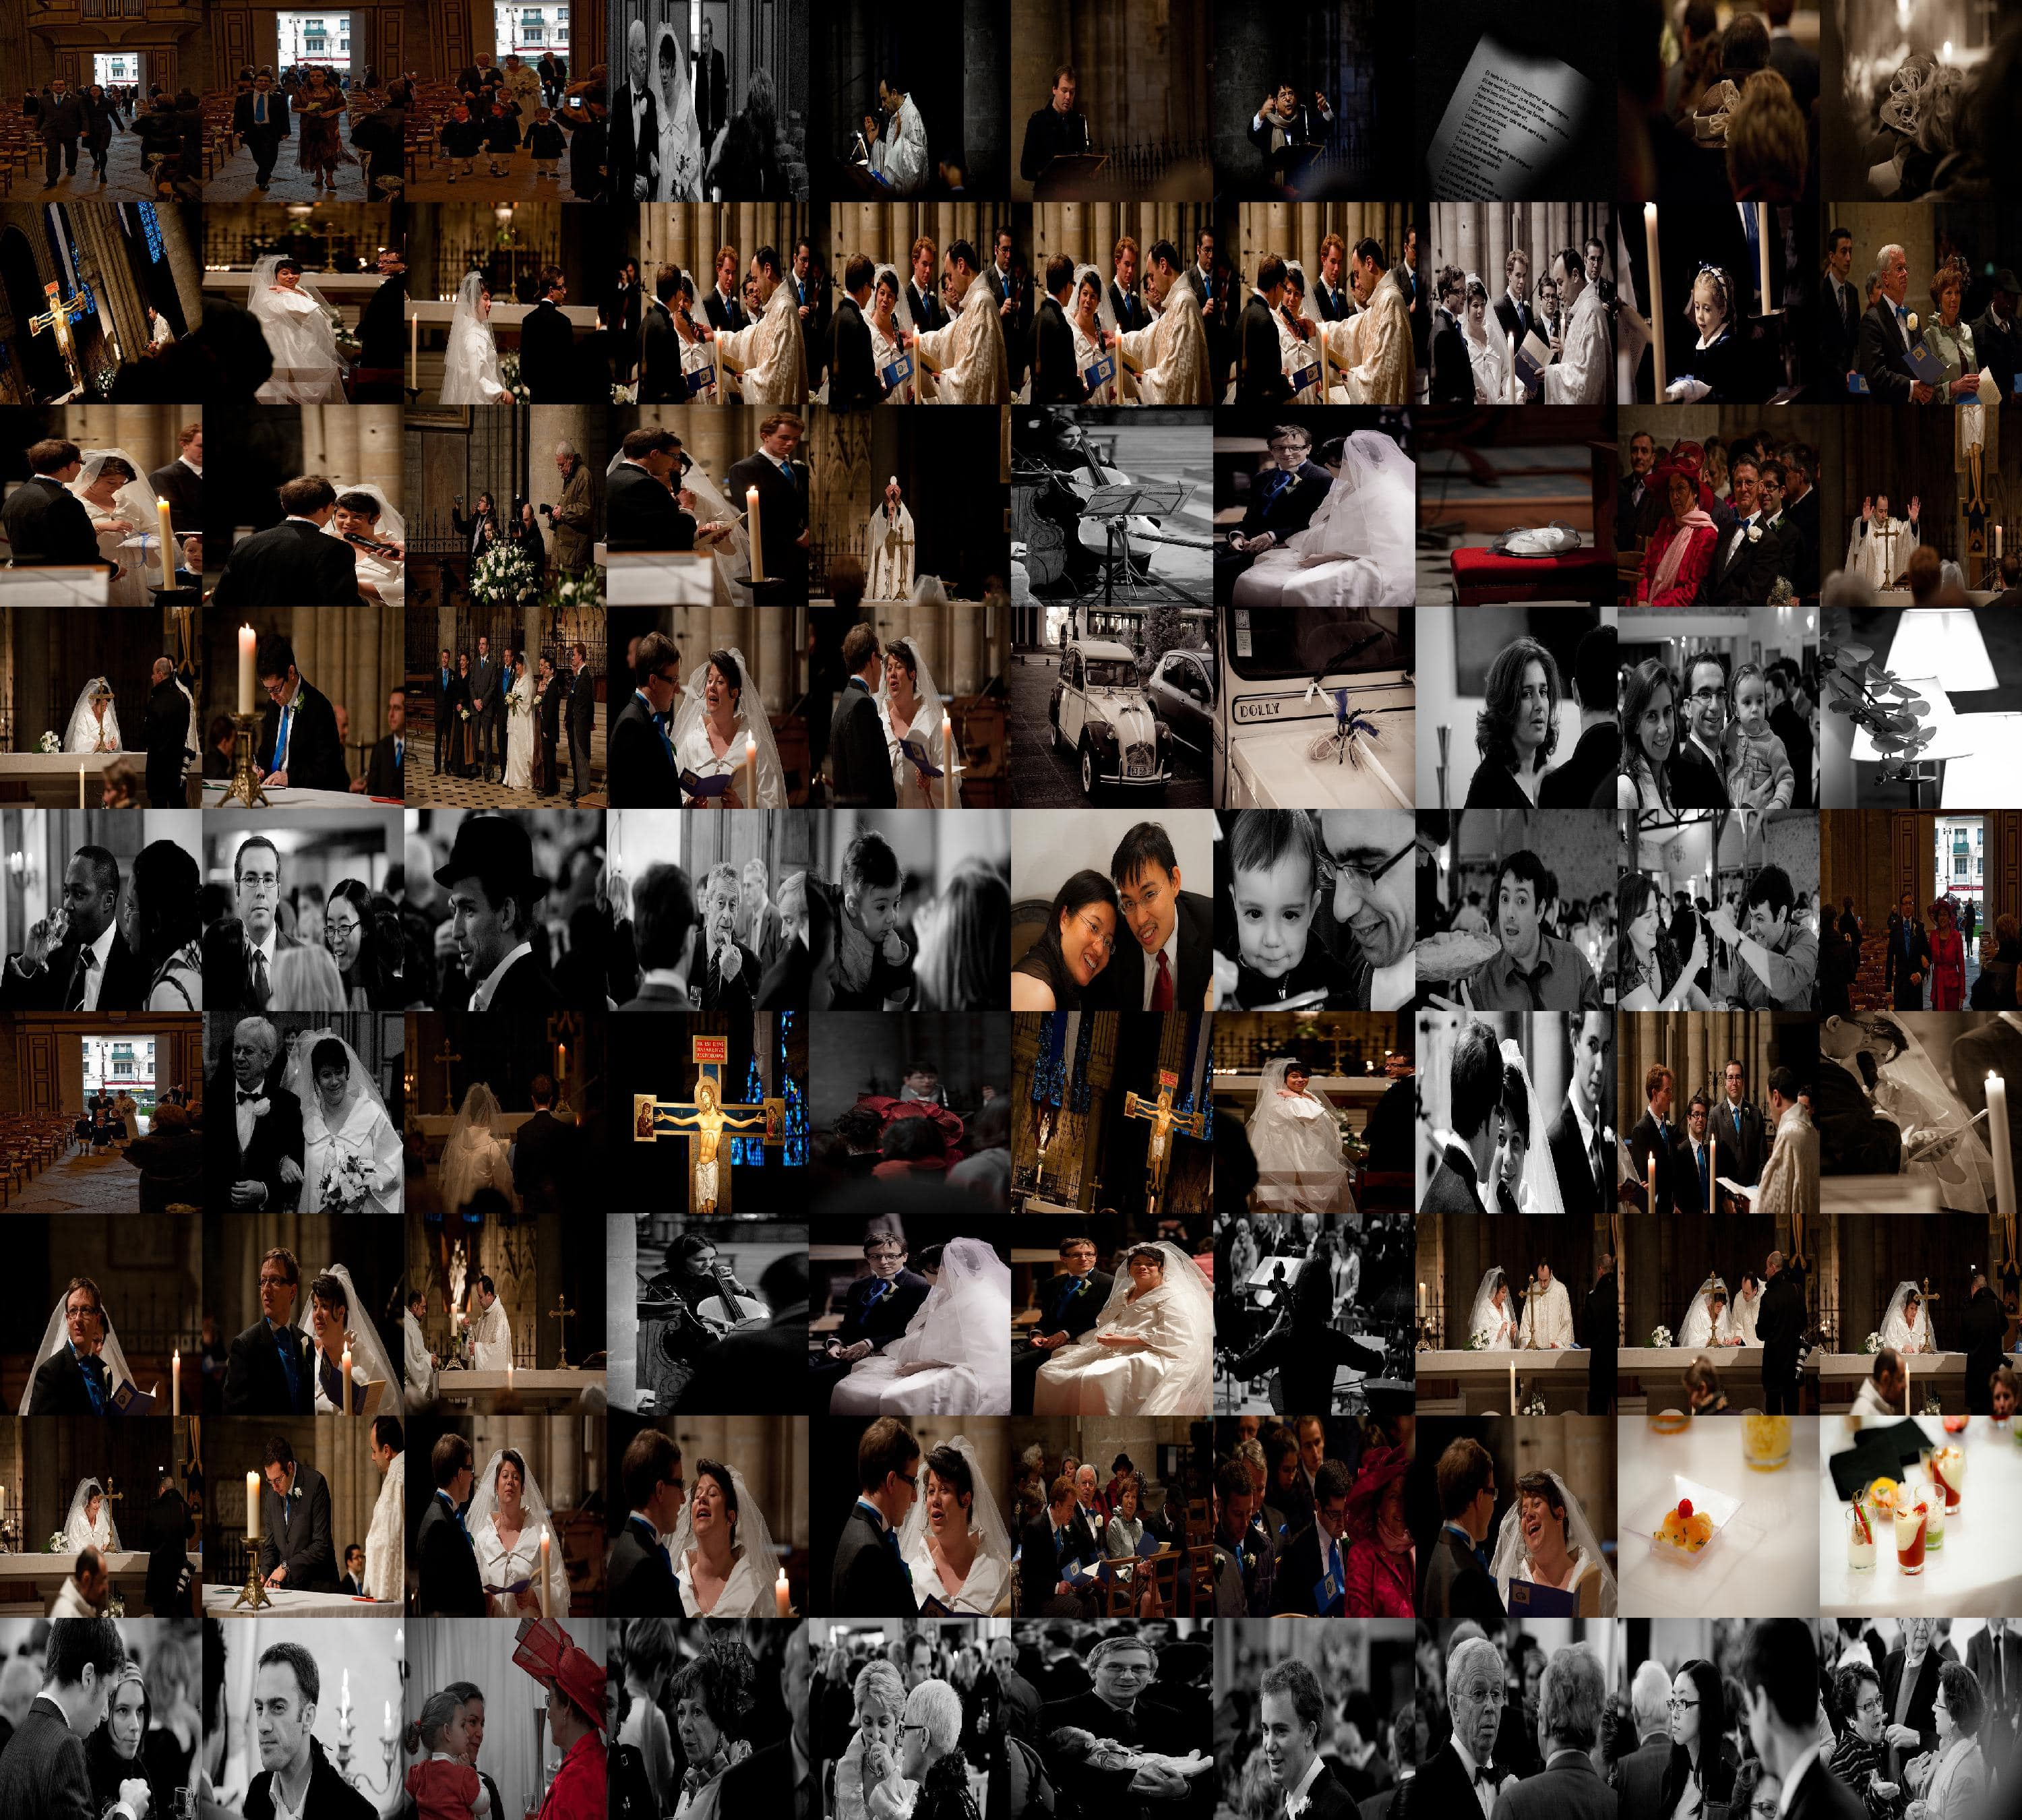
\includegraphics[width=\linewidth]{wedding_canvas}
  \caption{A \textit{Wedding} album. Spearman's Correlation $\rho = 0.78$, Kendall's $W = 0.64$}
  \label{wedding_album}
\end{subfigure}
\begin{subfigure}{0.49\textwidth}
  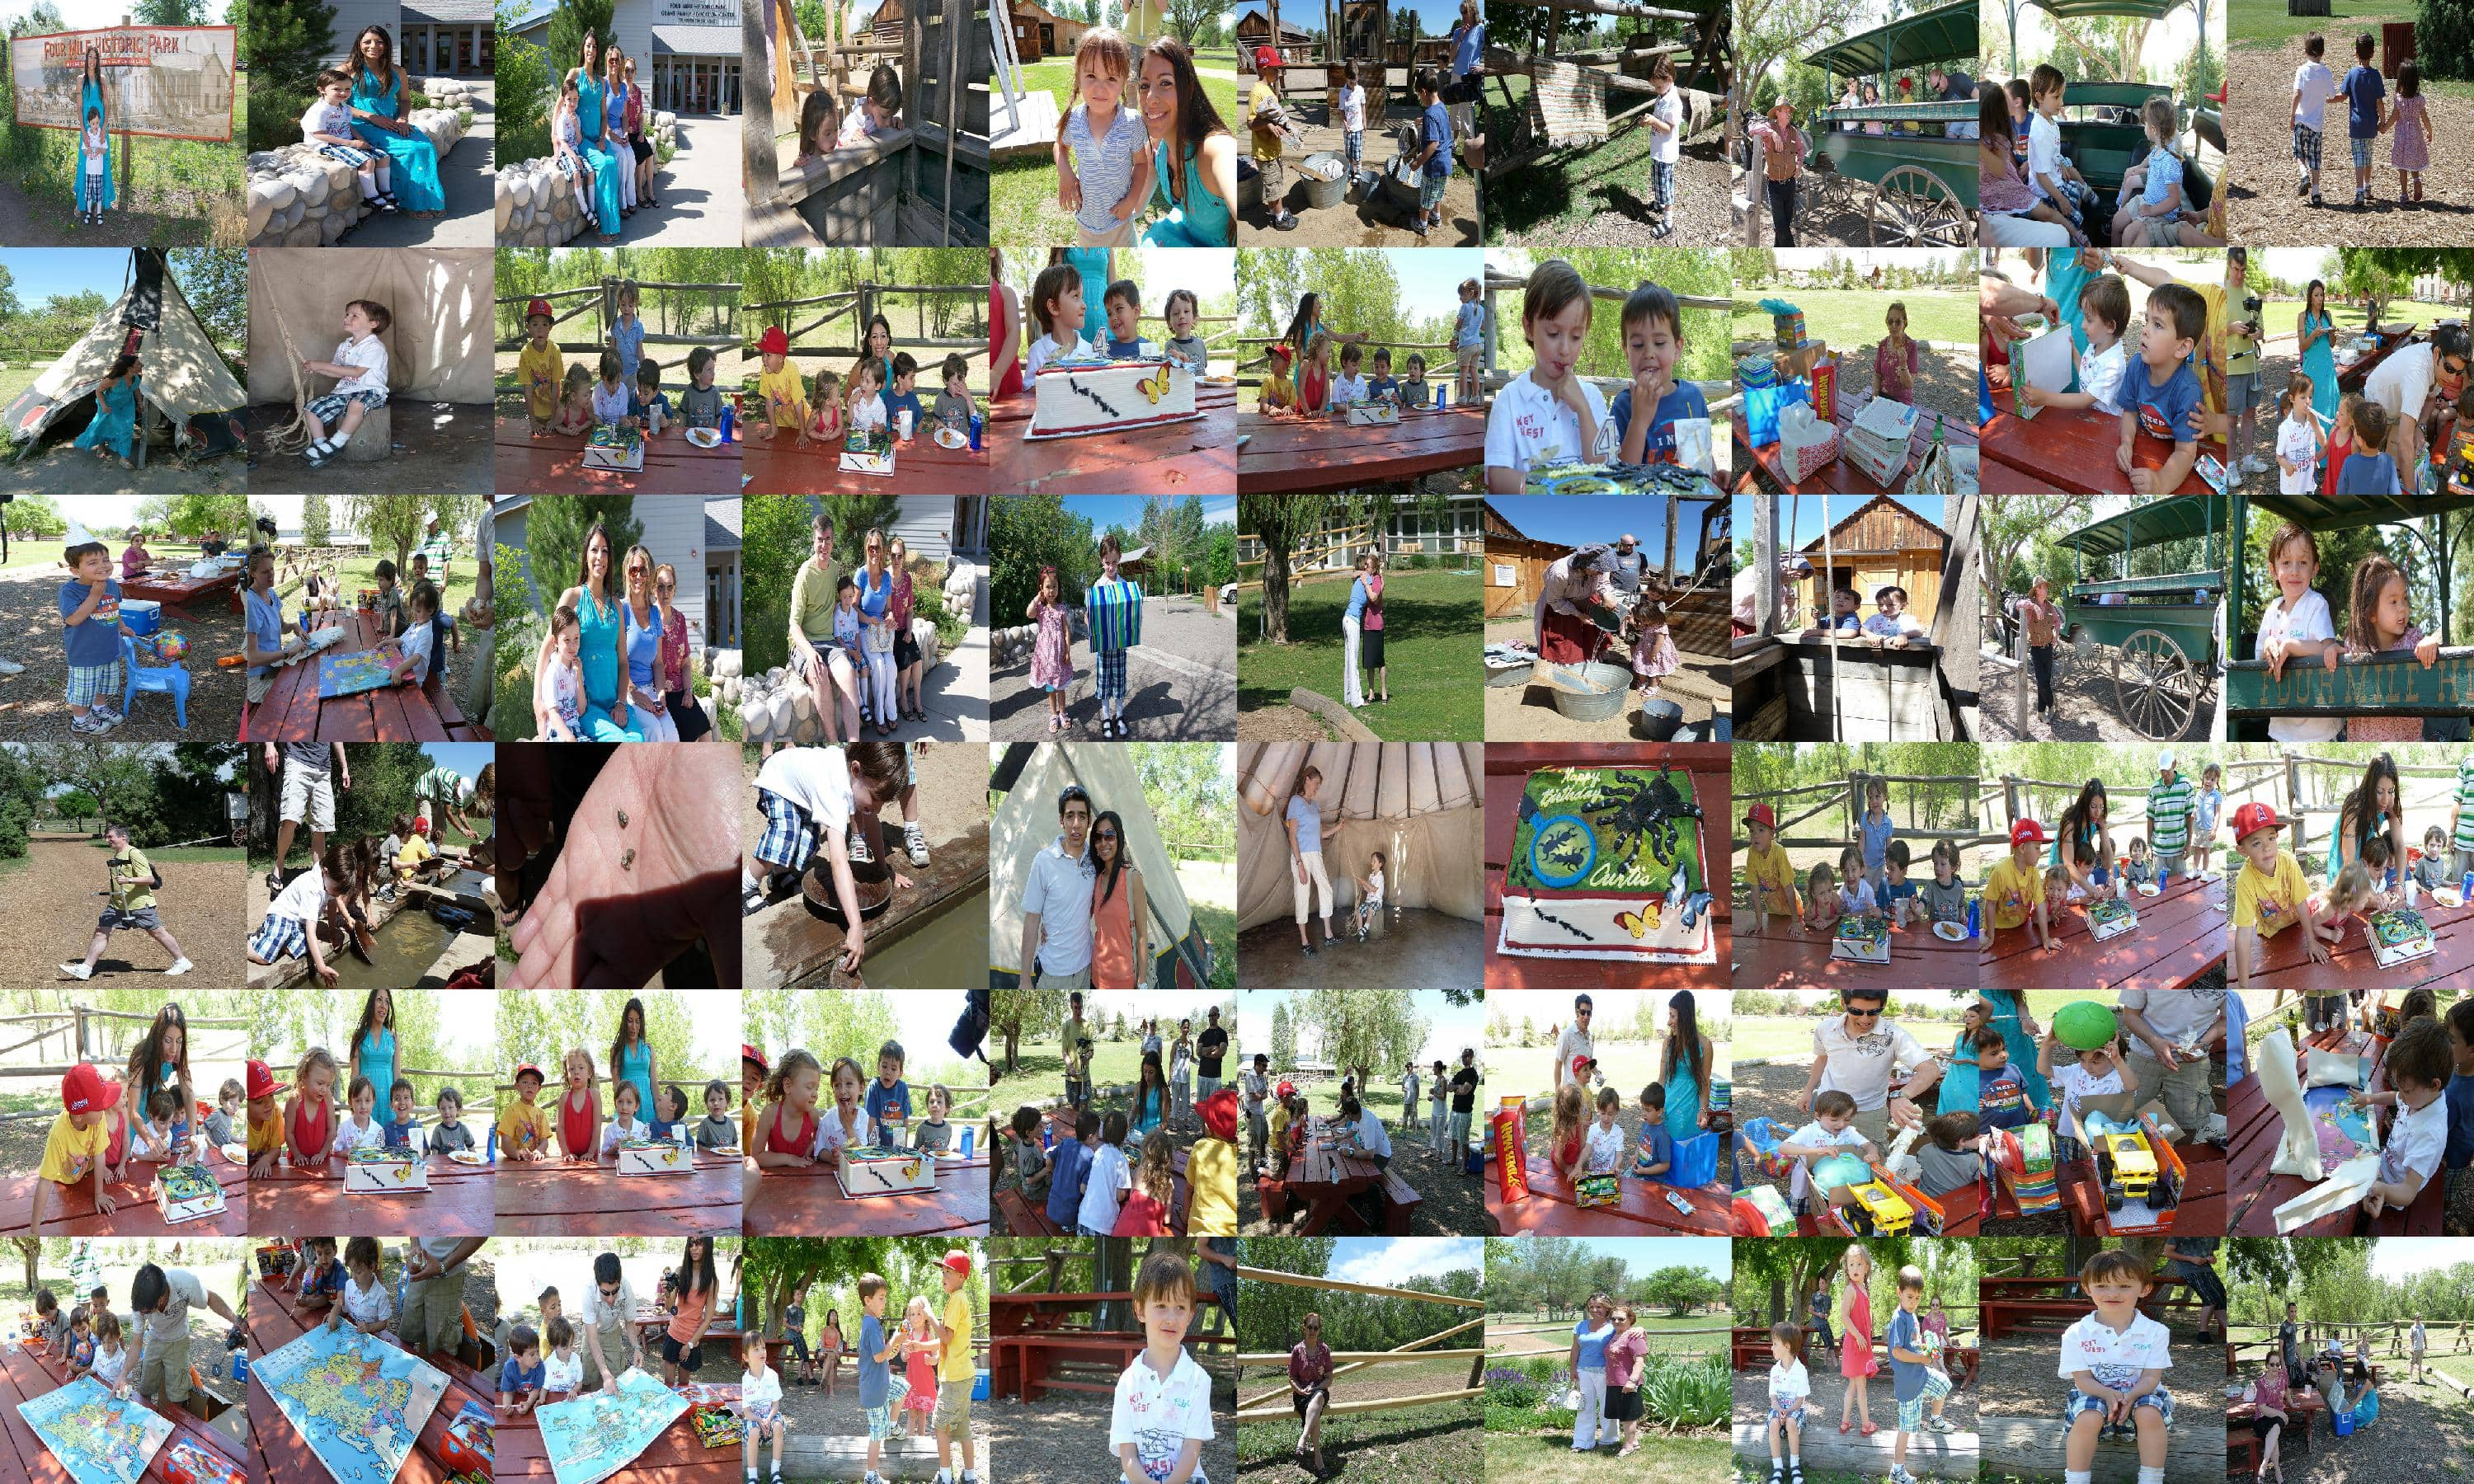
\includegraphics[width=\linewidth]{birthday_canvas}
  \caption{A \textit{Birthday} album. Spearman's Correlation $\rho = 0.61$, Kendall's $W = 0.49$}
  \label{birthday_album}
\end{subfigure}
\\
\begin{subfigure}{0.49\textwidth}
  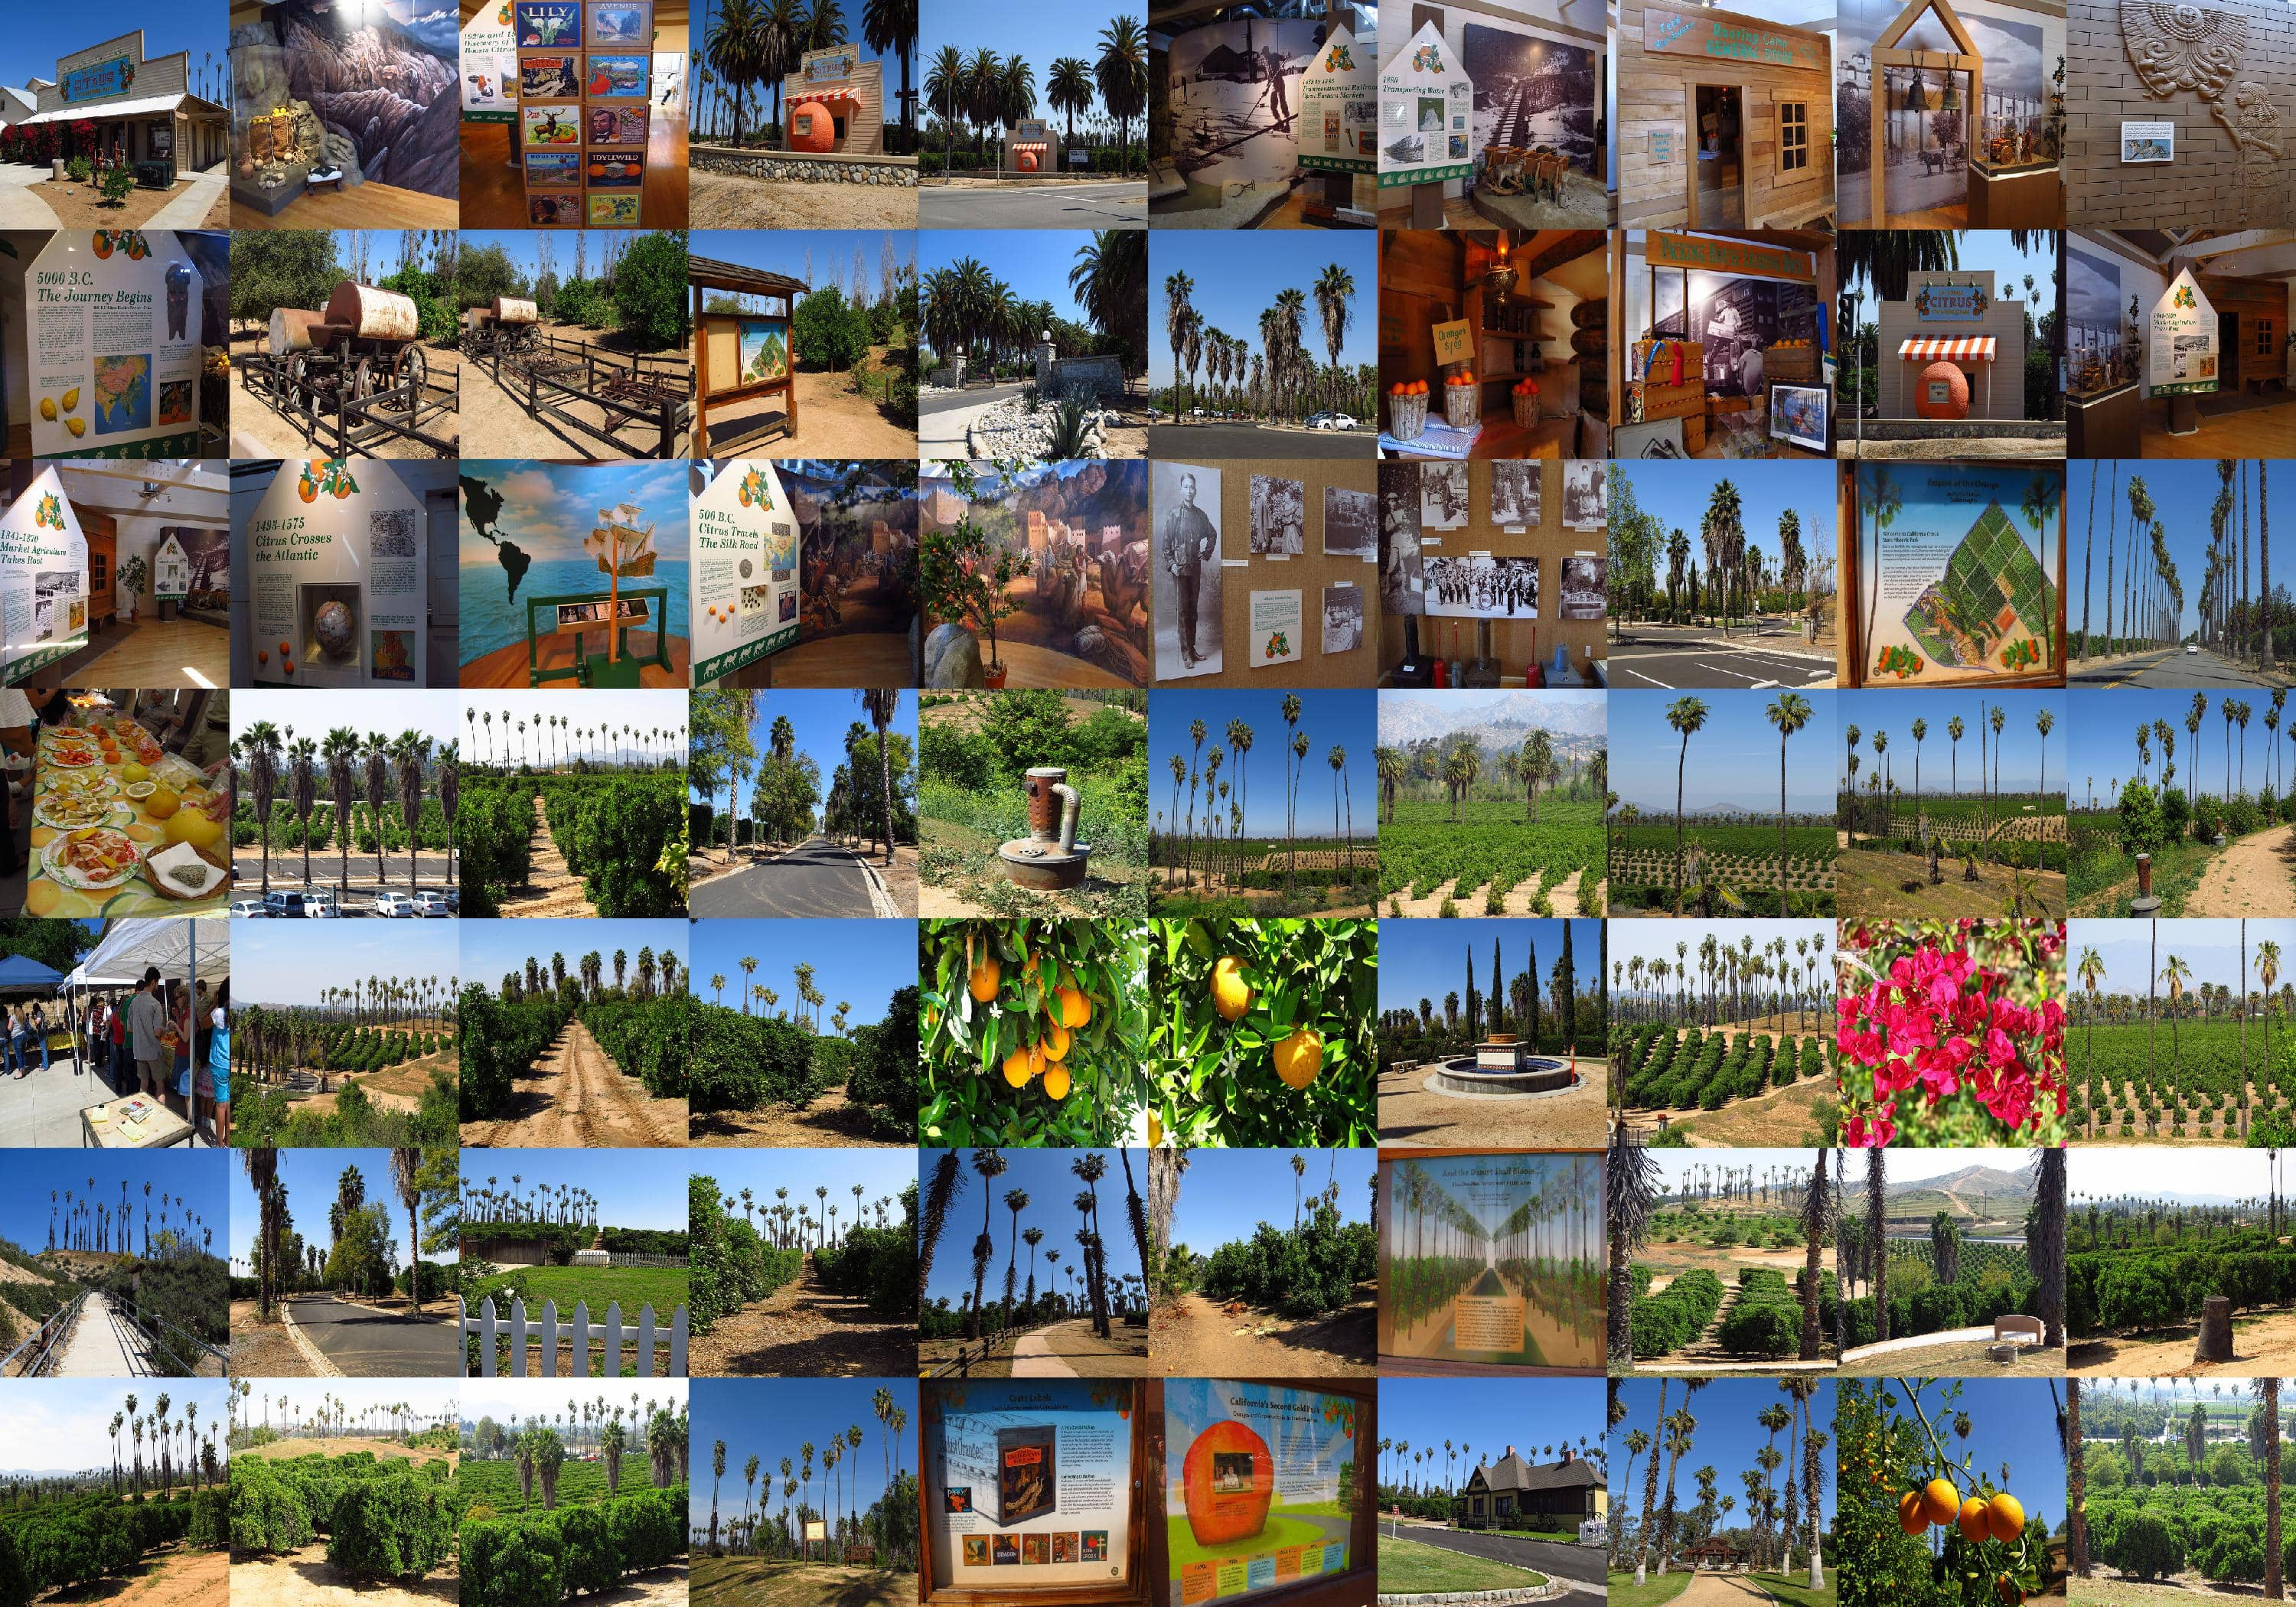
\includegraphics[width=\linewidth]{zoo_canvas}
%  \centering
  \caption{A \textit{Zoo/Botanic garden} album. Spearman's Correlation $\rho = 0.02$, Kendall's $W = 0.19$}
  \label{fig:sfig3}
\end{subfigure}
\begin{subfigure}{0.49\textwidth}
%  \centering
  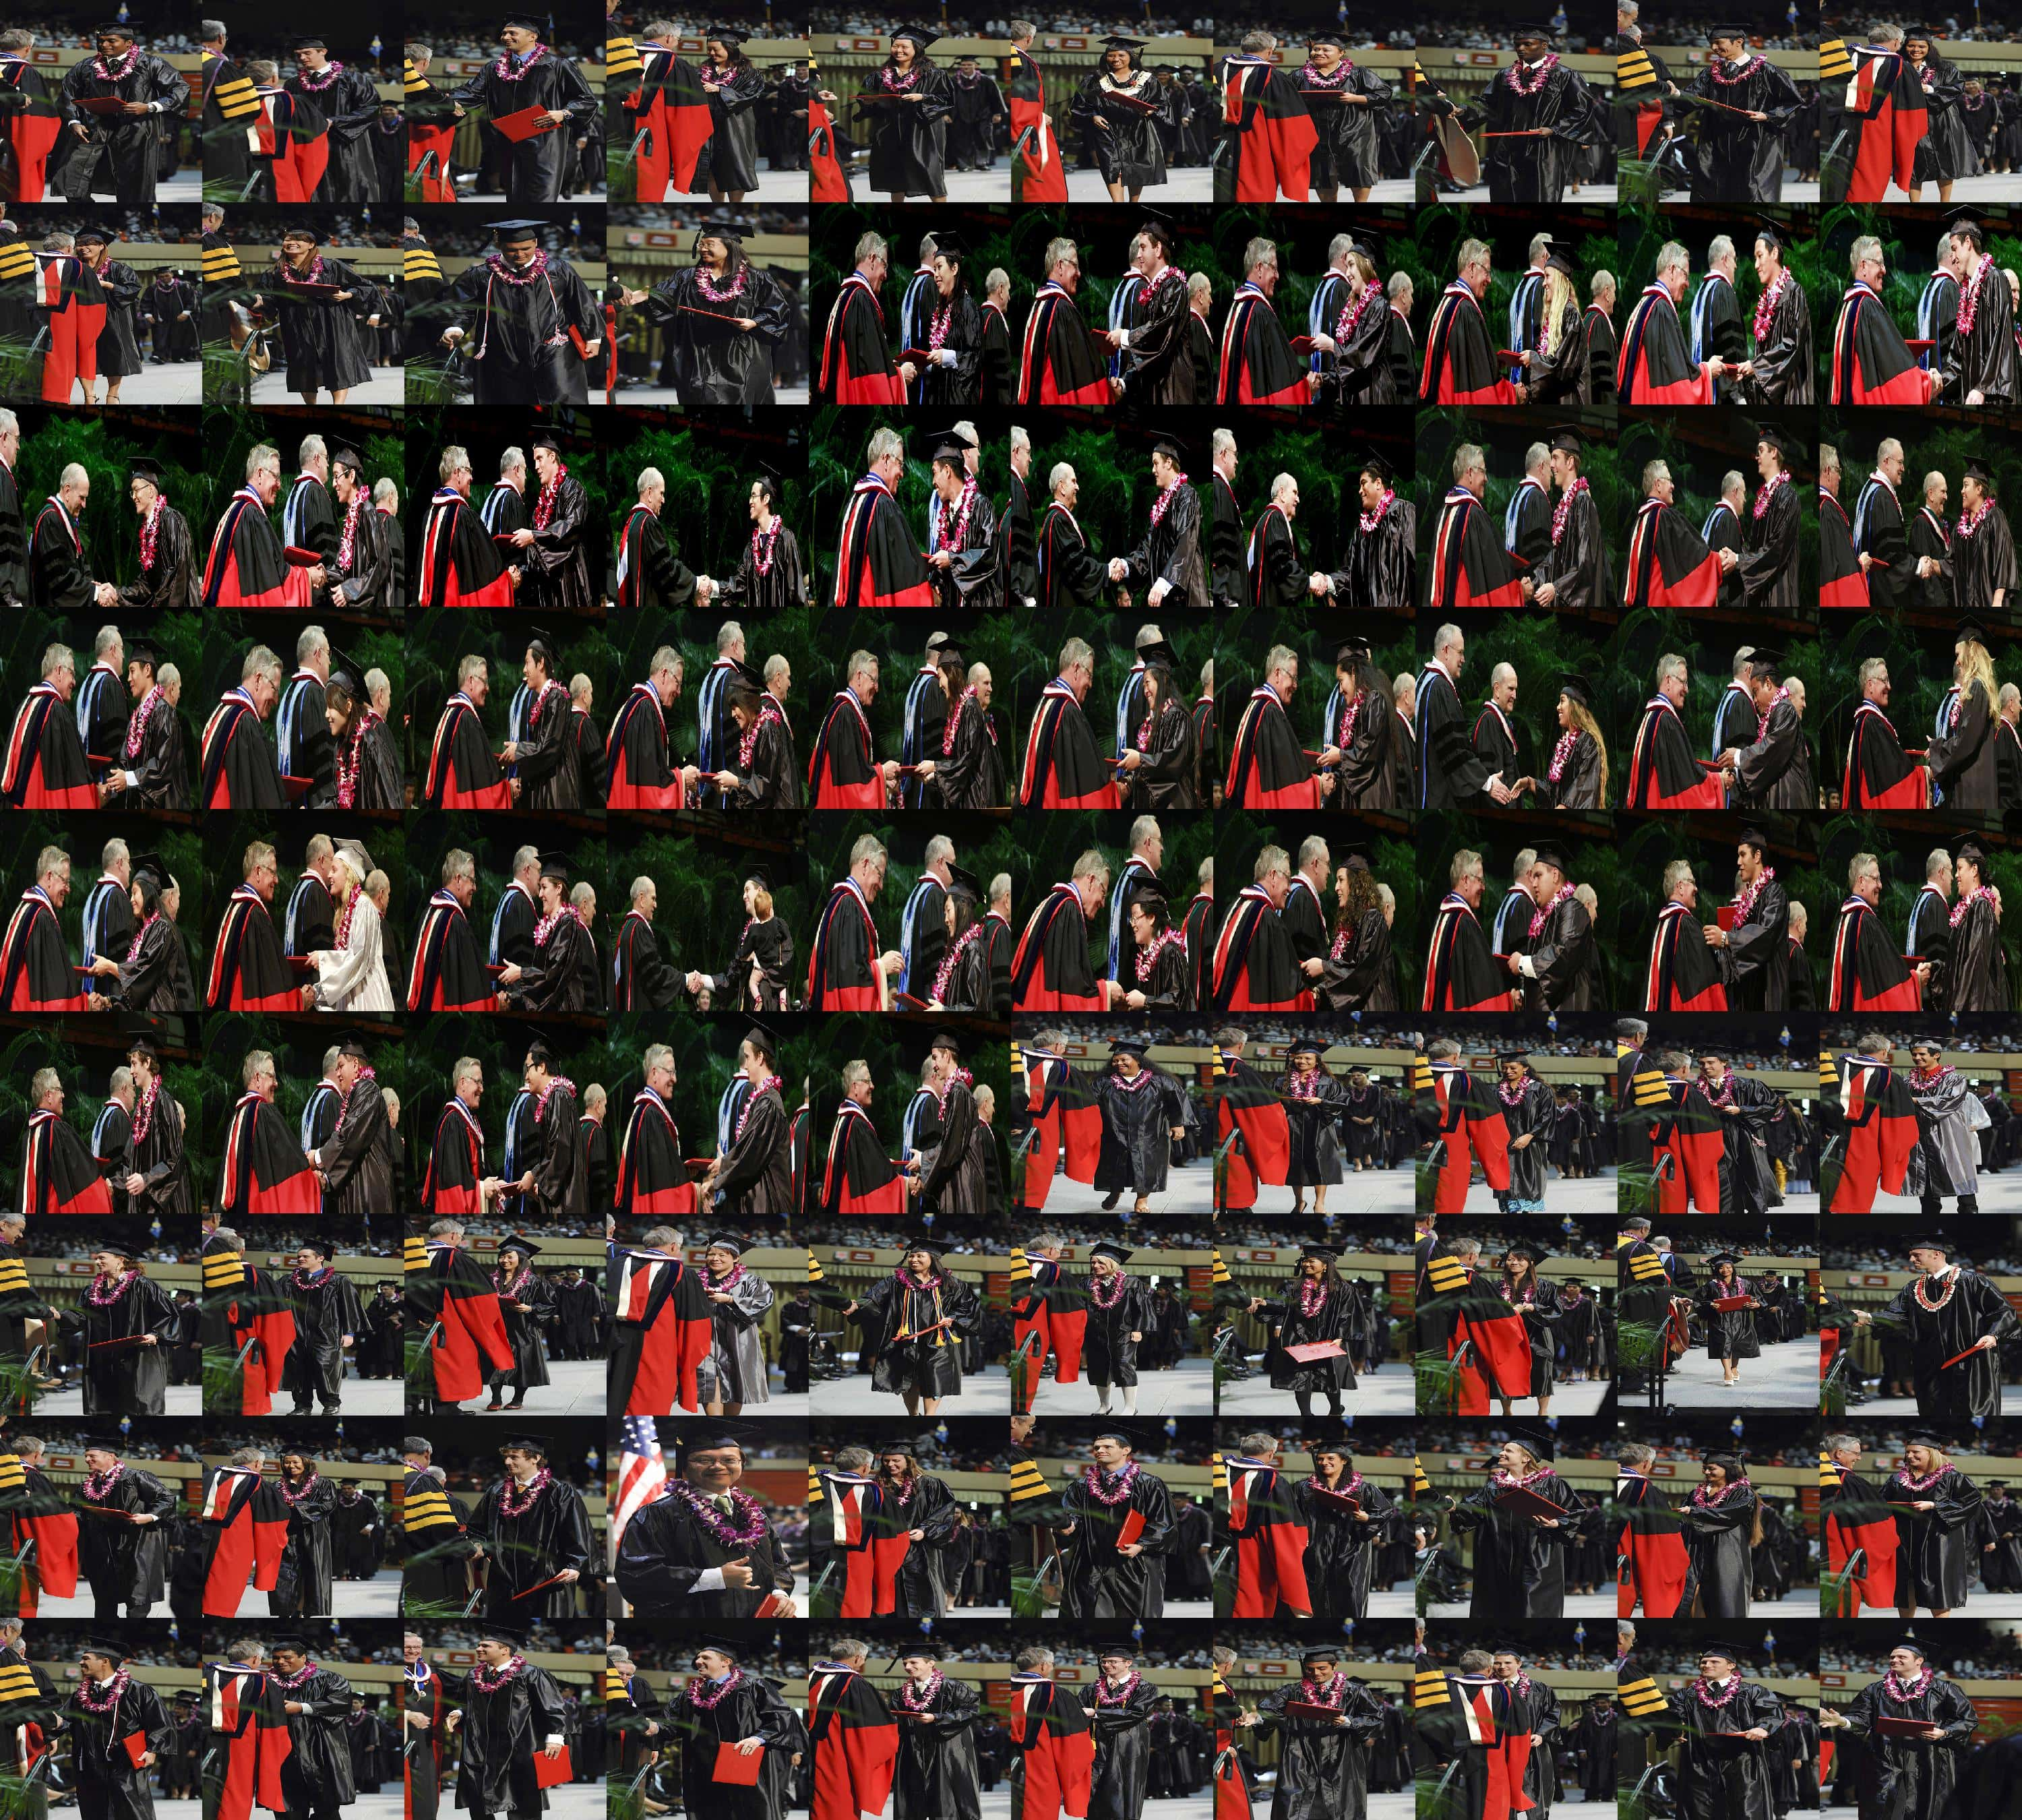
\includegraphics[width=\linewidth]{graduation_canvas}
  \caption{A \textit{Graduation} album.  Spearman's Correlation $\rho = -0.09$, Kendall's $W = 0.17$}
  \label{fig:sfig4}
\end{subfigure}
%\end{center}
\caption{Examples of albums in our dataset and the Spearman's Correlation $\rho$ and Kendall's $W$ from worker's rating for each album.}
\label{figure2}
\end{figure*}

\section{Architecture of Face Heatmap CNN}
In the main paper, we mentioned that the face heatmap CNN uses the similar siamese CNN architecture to train simultaneously for 23 event types. Here in Figure~\ref{face_figure}, we show the exact architecture we used for Face Heatmap network. 

\begin{figure*}[ht]
\begin{center}
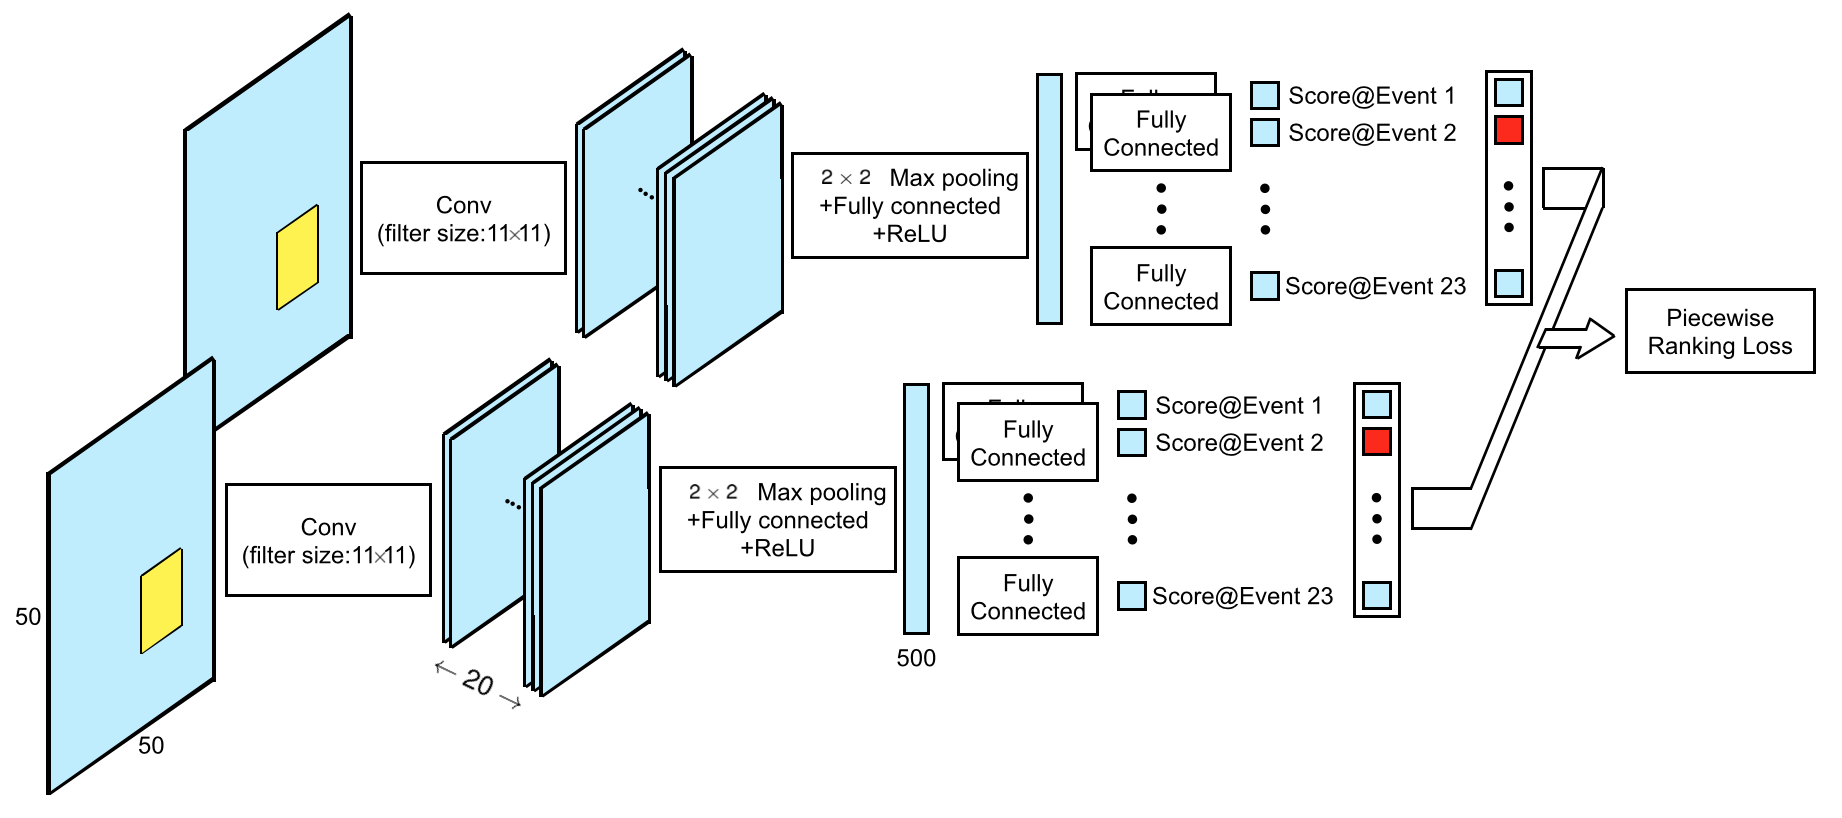
\includegraphics[width=0.8\textwidth]{face_heatmap}
\end{center}
\caption{Face Heatmap CNN architecture}
\label{face_figure}
\end{figure*}

\section{Result}
In this section, we present both quantitative results and qualitative results in addition to the main paper. 
\subsection{Quantitative Results}
%\textcolor{red}{Here I have two figures: Figure~\ref{figure5} and Figure~\ref{figure6_worker} for you to choose. ~\ref{figure5} doesn't include AMT worker's performance, while the other does.}
In Figure~\ref{bar_result_event_type}, we show the comparison of $\text{MAP}@t\%5$ by six methods for each of the 23 event types. The six methods being compared are: random ranking, aesthetics, K nearest neighbors with pre-trained CNN features (KNN), single network with Euclidean loss (Euclidean), siamese network with ranking SVM loss (Ranking-SVM), and our method using Ensemble of siamese CNNs (Ensemble). We also show a ``worker" method here for comparison. It is calculated as follows: for each album, we have 5 rankings from 5 workers, and we can calculate the MAP score for each worker's rating against the ground truth. Then all the MAPs over all albums are averaged for one event type. The ``worker" method is to measure how workers did on those albums.

As shown, our method outperforms all the other methods in most cases, except for \textit{Personal Art Activity}, \textit{Architecture},  \textit{Business Activity},  \textit{Protest} and  \textit{Nature Trip}. Our method can even beat ``worker" in some cases.

As mentioned in the main paper, the aesthetic score doesn't perform well overall, however, it has good performance on two event types: \textit{Personal Art Activity} and \textit{Nature Trip}. Especially for \textit{Nature Trip}, aesthetics achieves the best performance over all methods. 

\begin{figure*}[ht]
\begin{center}
\makebox[\linewidth][c]{
\begin{subfigure}{\textwidth}
  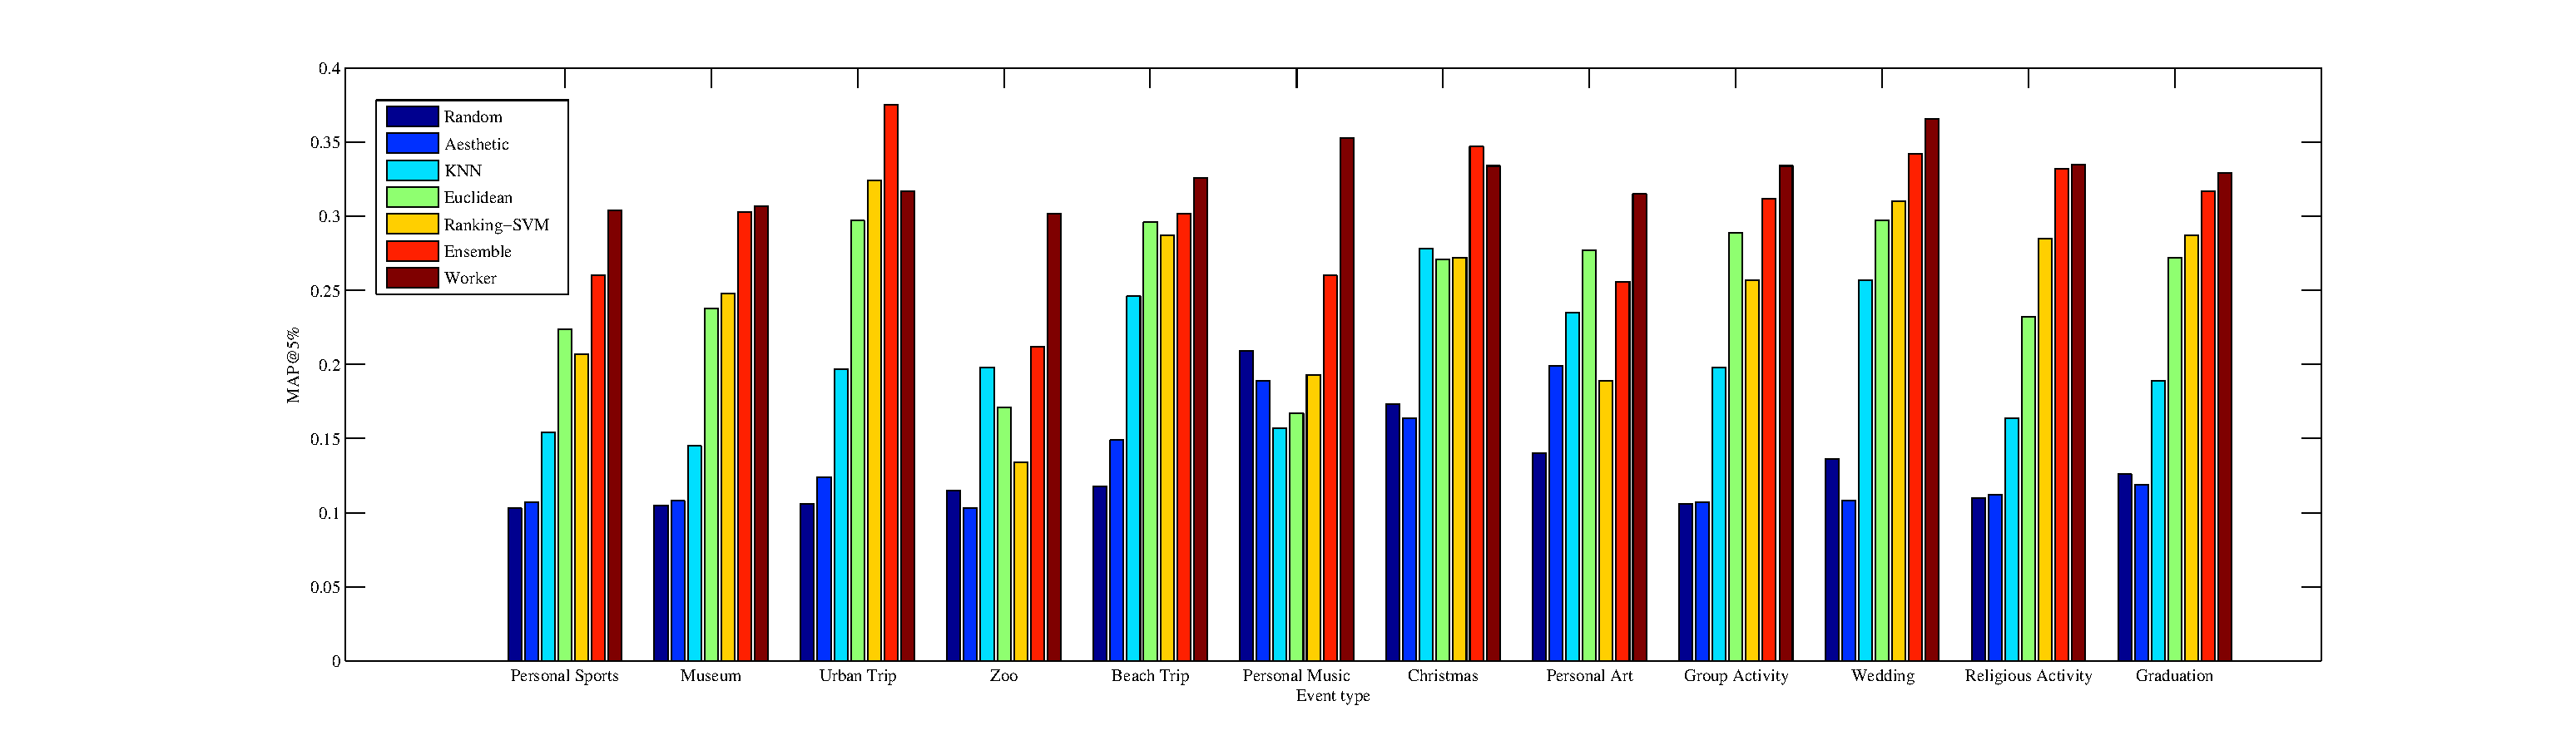
\includegraphics[width=\linewidth]{5_worker_1}
  \centering
%  \caption{1a}
  \label{fig:sfig1_worker}
\end{subfigure}
}
\\
\makebox[\linewidth][c]{
\begin{subfigure}{\textwidth}
  \centering
  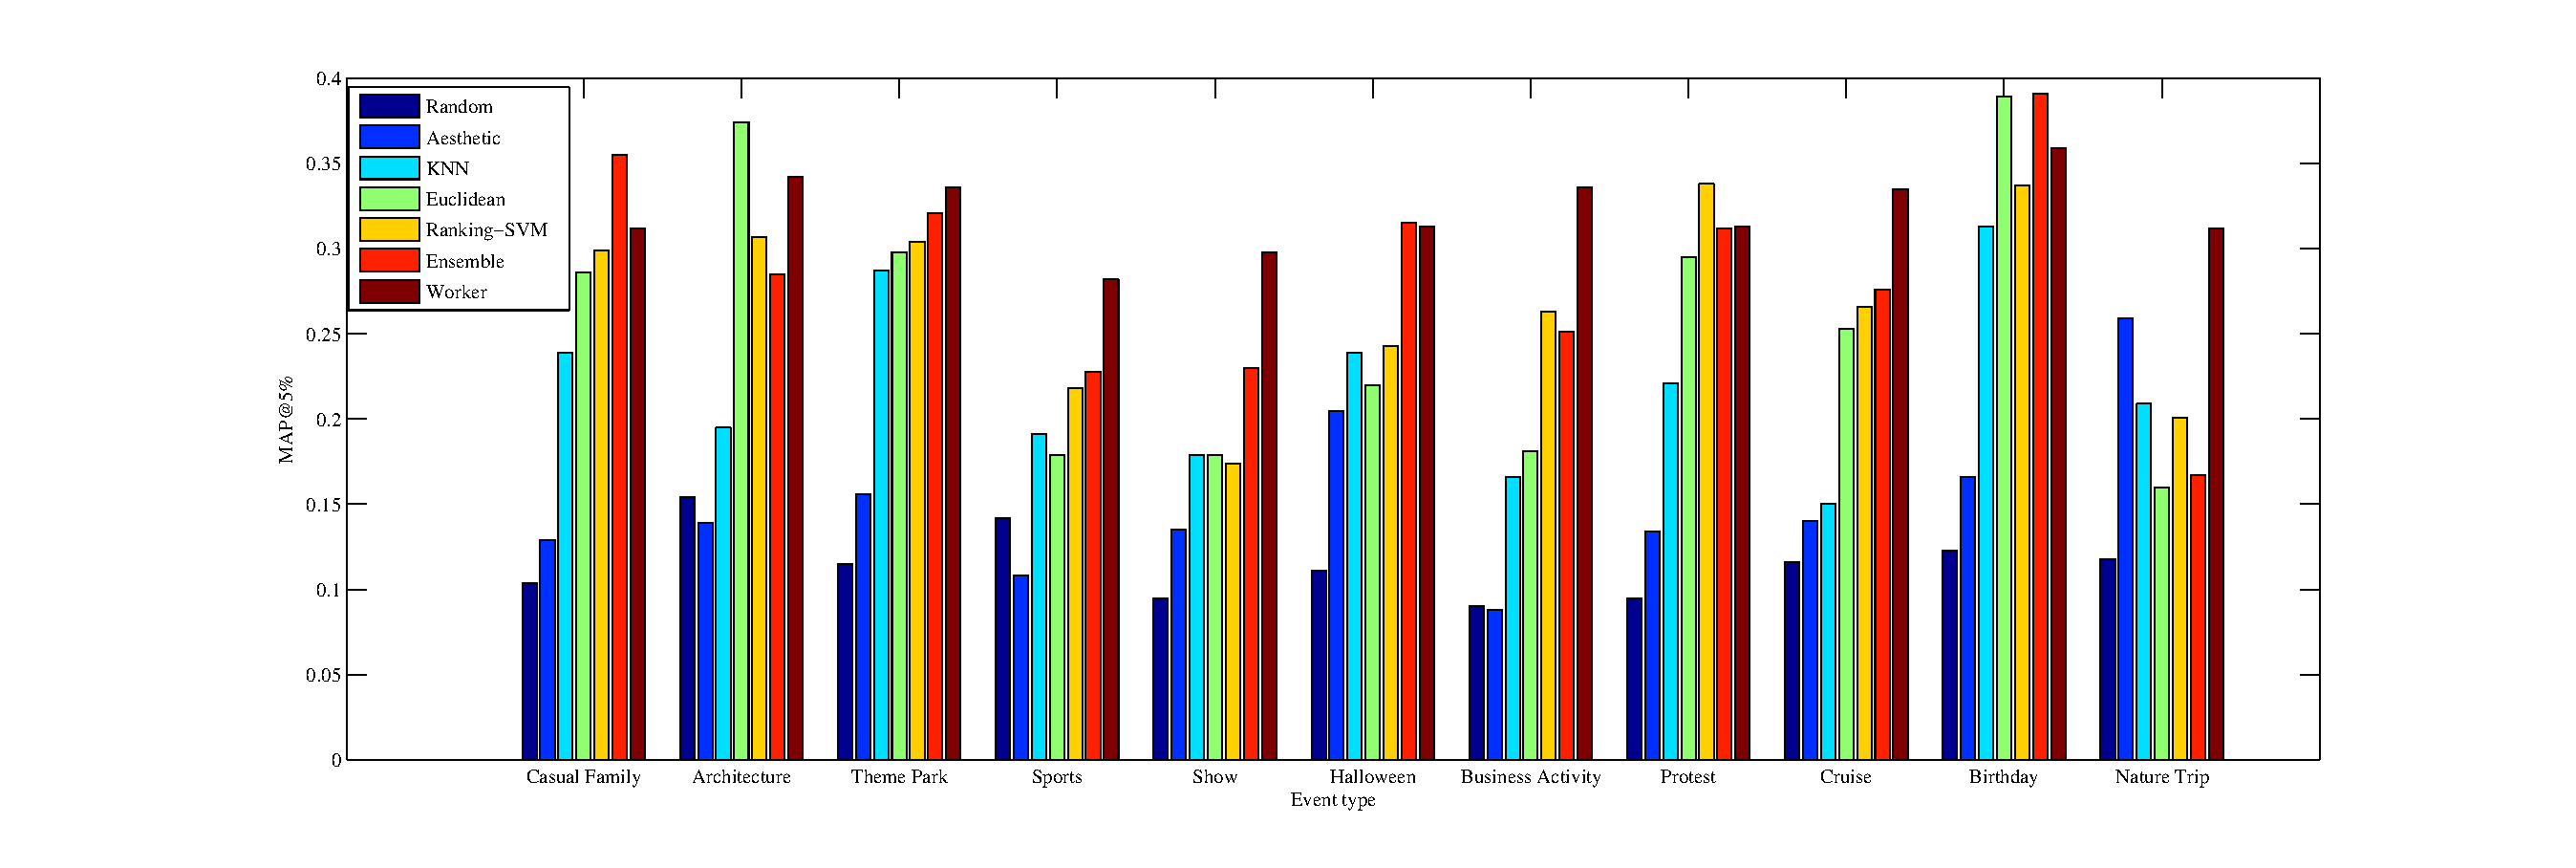
\includegraphics[width=\linewidth]{5_worker_2}
%  \caption{1b}
  \label{fig:sfig2_worker}
\end{subfigure}
}
\end{center}
\caption{Comparison of six methods for 23 event types respectively. Individual worker's performance is also included as comparison. Results of $\text{MAP}@t\%5$ are shown.}
\label{bar_result_event_type}
\end{figure*}

In the main paper, we mentioned that we used grid search on 5-fold cross validation to decide the parameters $\{\alpha, \beta, \lambda\}$ to incorporate the face heatmap. Among 23 event types, only 10 event types showed a performance gain after face information was incorporated in the validation set, and therefore face information was only used for these 10 event types. Table~\ref{face_table} shows the effect of incorporating face information for these 10 event types.

In Table~\ref{aesthetic_table}, we show the comparison of the results from single network with Euclidean loss (Euclidean), our method using Ensemble of siamese CNNs (Ensemble-CNN), and our method  after incorporating face information (Ensemble-CNN + face). This is in addition to the result table we presented in the main paper.  As mentioned in the main paper, with face information, $\text{MAP}$ is slightly improved by about 0.1\%, and the face heatmap network helped very little.

\clearpage
\begin{table*}[t]
\small
\centerline{
\begin{tabular}{c|C{3cm}C{3cm}C{3cm}}
\hline
%\multicolumn{1}{l|}{} & \multicolumn{3}{c}{$\text{MAP}@t\%$}          \\ \hline
t\%                   & 5             & 15            & 25            \\ \hline
Beach Trip            & 0.353(+0.051) & 0.455(+0.022) & 0.555(+0.011) \\
Nature Trip            & 0.167(+0.008) & 0.272(+0.008) & 0.369(+0.007) \\
Group Activity            & 0.315(+0.003) & 0.489(+0.001) & 0.586(+0.003) \\
Halloween            & 0.315(+0.000) & 0.424(+0.001) & 0.529(+0.002) \\ 
Personal Art Activity   & 0.256(+0.000) & 0.361(0.002) & 0.449(+0.000) \\ 
Religious Activity  & 0.320(-0.012) & 0.416(0.000) & 0.503(+0.005) \\ 
Graduation  & 0.317(+0.001) & 0.444(0.002) & 0.548(+0.001) \\ 
Sports  & 0.228(+0.001) & 0.322(0.002) & 0.420(+0.002) \\ 
Show  & 0.232(+0.002) & 0.356(0.002) & 0.473(+0.001) \\ 
Museum            & 0.293(-0.010) & 0.367(-0.010) & 0.453(-0.006) \\\hline
\end{tabular}
}
\caption{For a given event type, $\text{MAP}@t\%$ for the Ensemble-CNN after using the face information. The difference between before v.s. after face information is shown in parentheses. All the 10 event types for which face information is used are shown here.}
\label{face_table}
\end{table*}

\begin{table*}[t]
\small
\begin{tabular}{c|cccccc|cccccc}
\hline
          & \multicolumn{6}{c|}{$\text{MAP}@t\%$}          & \multicolumn{6}{c}{$P@t\%$} \\ \hline  \hline
t\%       & 5     & 10    & 15    & 20    & 25    & 30    & 5  & 10  & 15 & 20 & 25 & 30 \\ \hline
Euclidean & 0.266&0.329 & 0.389 & 0.444 & 0.494 & 0.540  & 0.173  &  0.260   &  0.328  &  0.391  & 0.439   & 0.485   \\
Ensemble-CNN & 0.305& 0.364& 0.417& 0.471& 0.519&0.563& 0.216&0.301& 0.360& 0.411&0.459&0.504 \\
Ensemble-CNN + face &0.306&0.364&0.418&0.472&0.520&0.563&0.215&0.303&0.360&0.413&0.460&0.503 \\ \hline
\end{tabular}
\caption{Comparison of predictions using different methods that weren't shown in the main paper. Evaluation metric here is $\text{MAP}@t\%$ and $P@t\%$.}
\label{aesthetic_table}
\end{table*}

\clearpage

\subsection{Qualitative Results}
In addition to the visual example of our method's performance in the main paper, we show more examples of our method. Here we present 64 examples from all 23 event types from Figure~\ref{fig11} to Figure~\ref{fig74}. For each album, we show top 10-20\% images of the album from three methods. For each method, the top photos returned are arranged in chronological	order.
(Each album has different size, while we want to constrain the number of images we show to make it easier to view.) First row is the ground truth we acquired from AMT worker; second row is our prediction using Ensemble-CNN which we introduced in the main paper; third row is the result from random selection. Note that the images are distorted for viewing.

 We can see that for most albums that have strong narrative structure or albums that consist of images that vary much in quality or semantics, our method's results are close to, though do not perfectly match the ground truth result; on the contrary, the results from random selection are obviously less appealing (for example,  Figure~\ref{fig11}, \ref{fig14}, \ref{fig36}, etc.).  For instance, in Figure~\ref{fig23}, our method captures the important moments of the wedding event, similar to those people picked (in the ground truth); however random selection has many images that are less important, for example, photos of people eating, or photos of guests talking, while not looking at the camera.
 
 There are also some albums in which most of the images are of similar quality or semantics, for example, Figure~\ref{fig17}, \ref{fig49}. 
 
 
\begin{figure*}[ht]
\centering
  \subcaptionbox{Top 20\% of a \textit{Wedding} album. \label{fig11}}{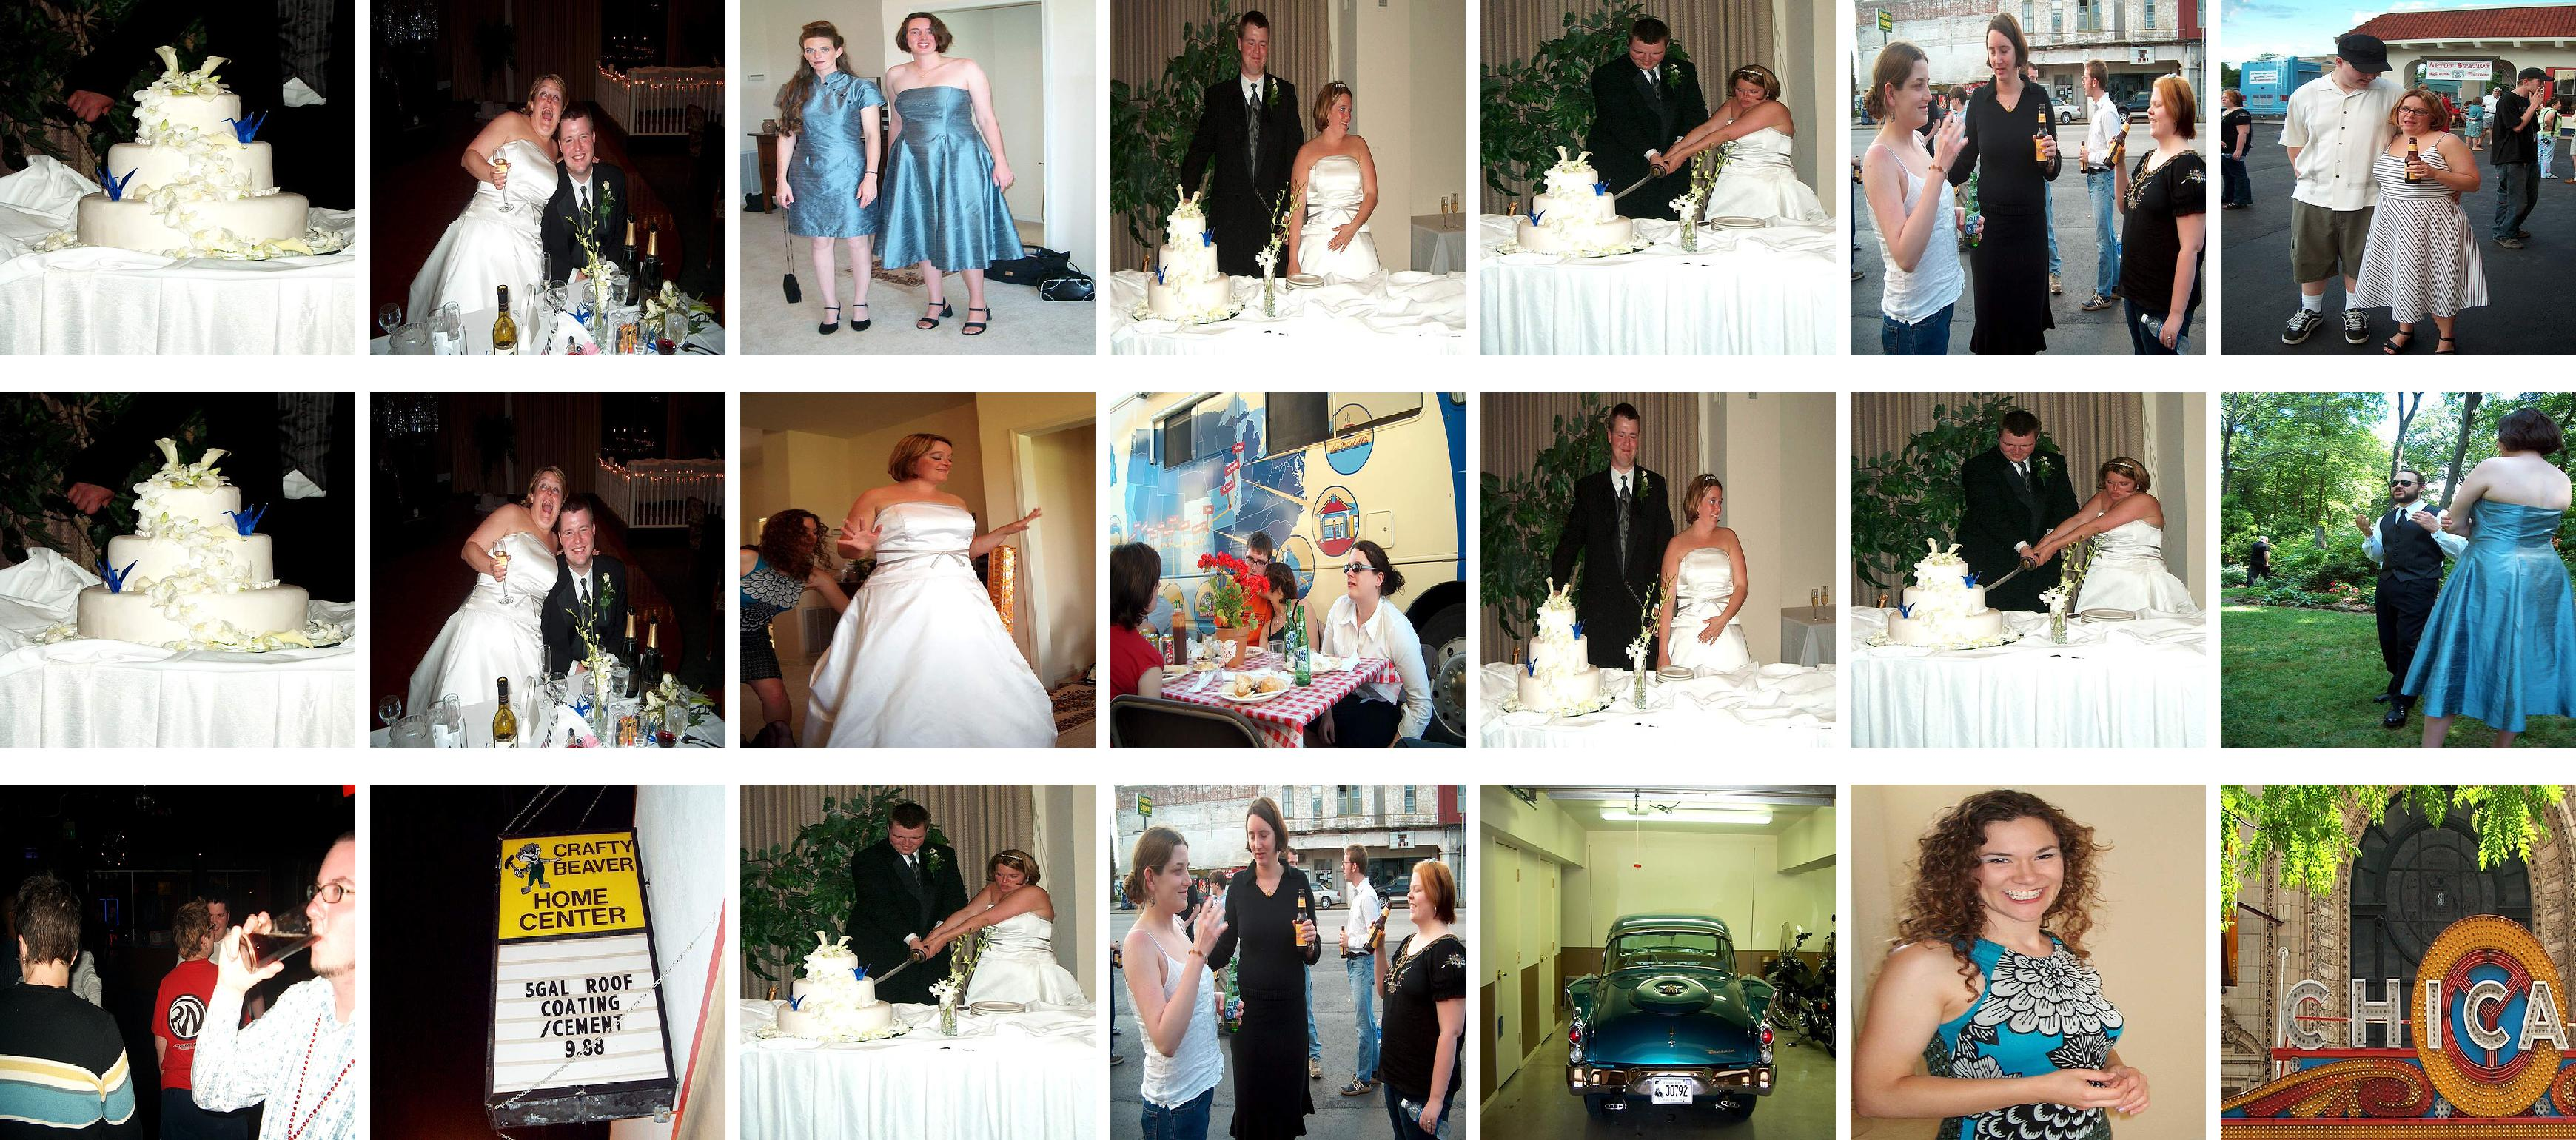
\includegraphics[height=1.5in]{results/a1_0_67618625@N00_7_20.jpg}}
  \subcaptionbox{Top 20\% of a \textit{Museum} album. \label{fig12}}{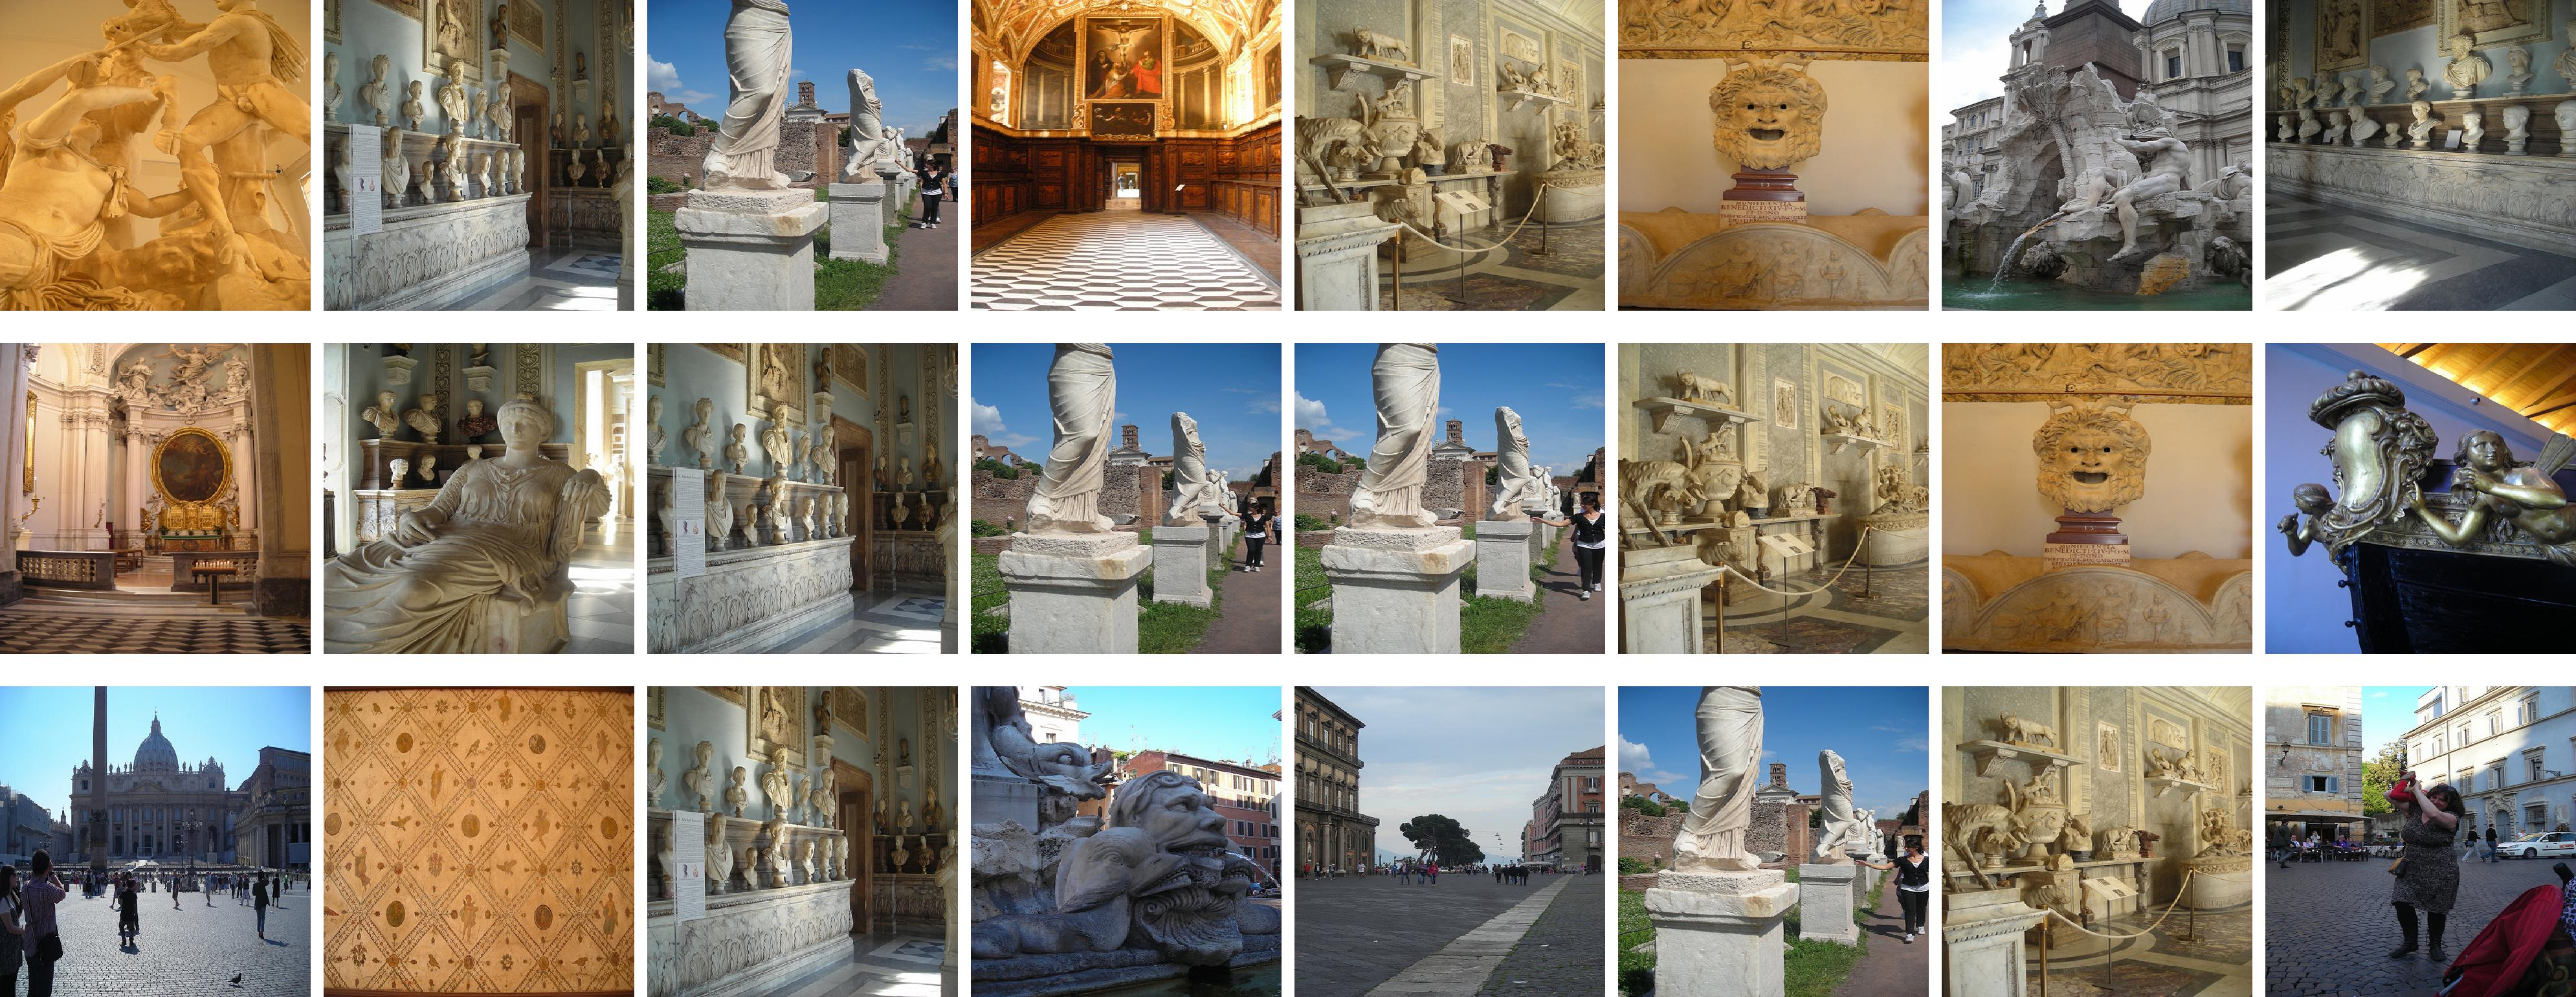
\includegraphics[height=1.5in]{results/a2_0_9137715@N05_8_20.jpg}}
  \subcaptionbox{Top 10\% of a \textit{Graduation} album. \label{fig13}}{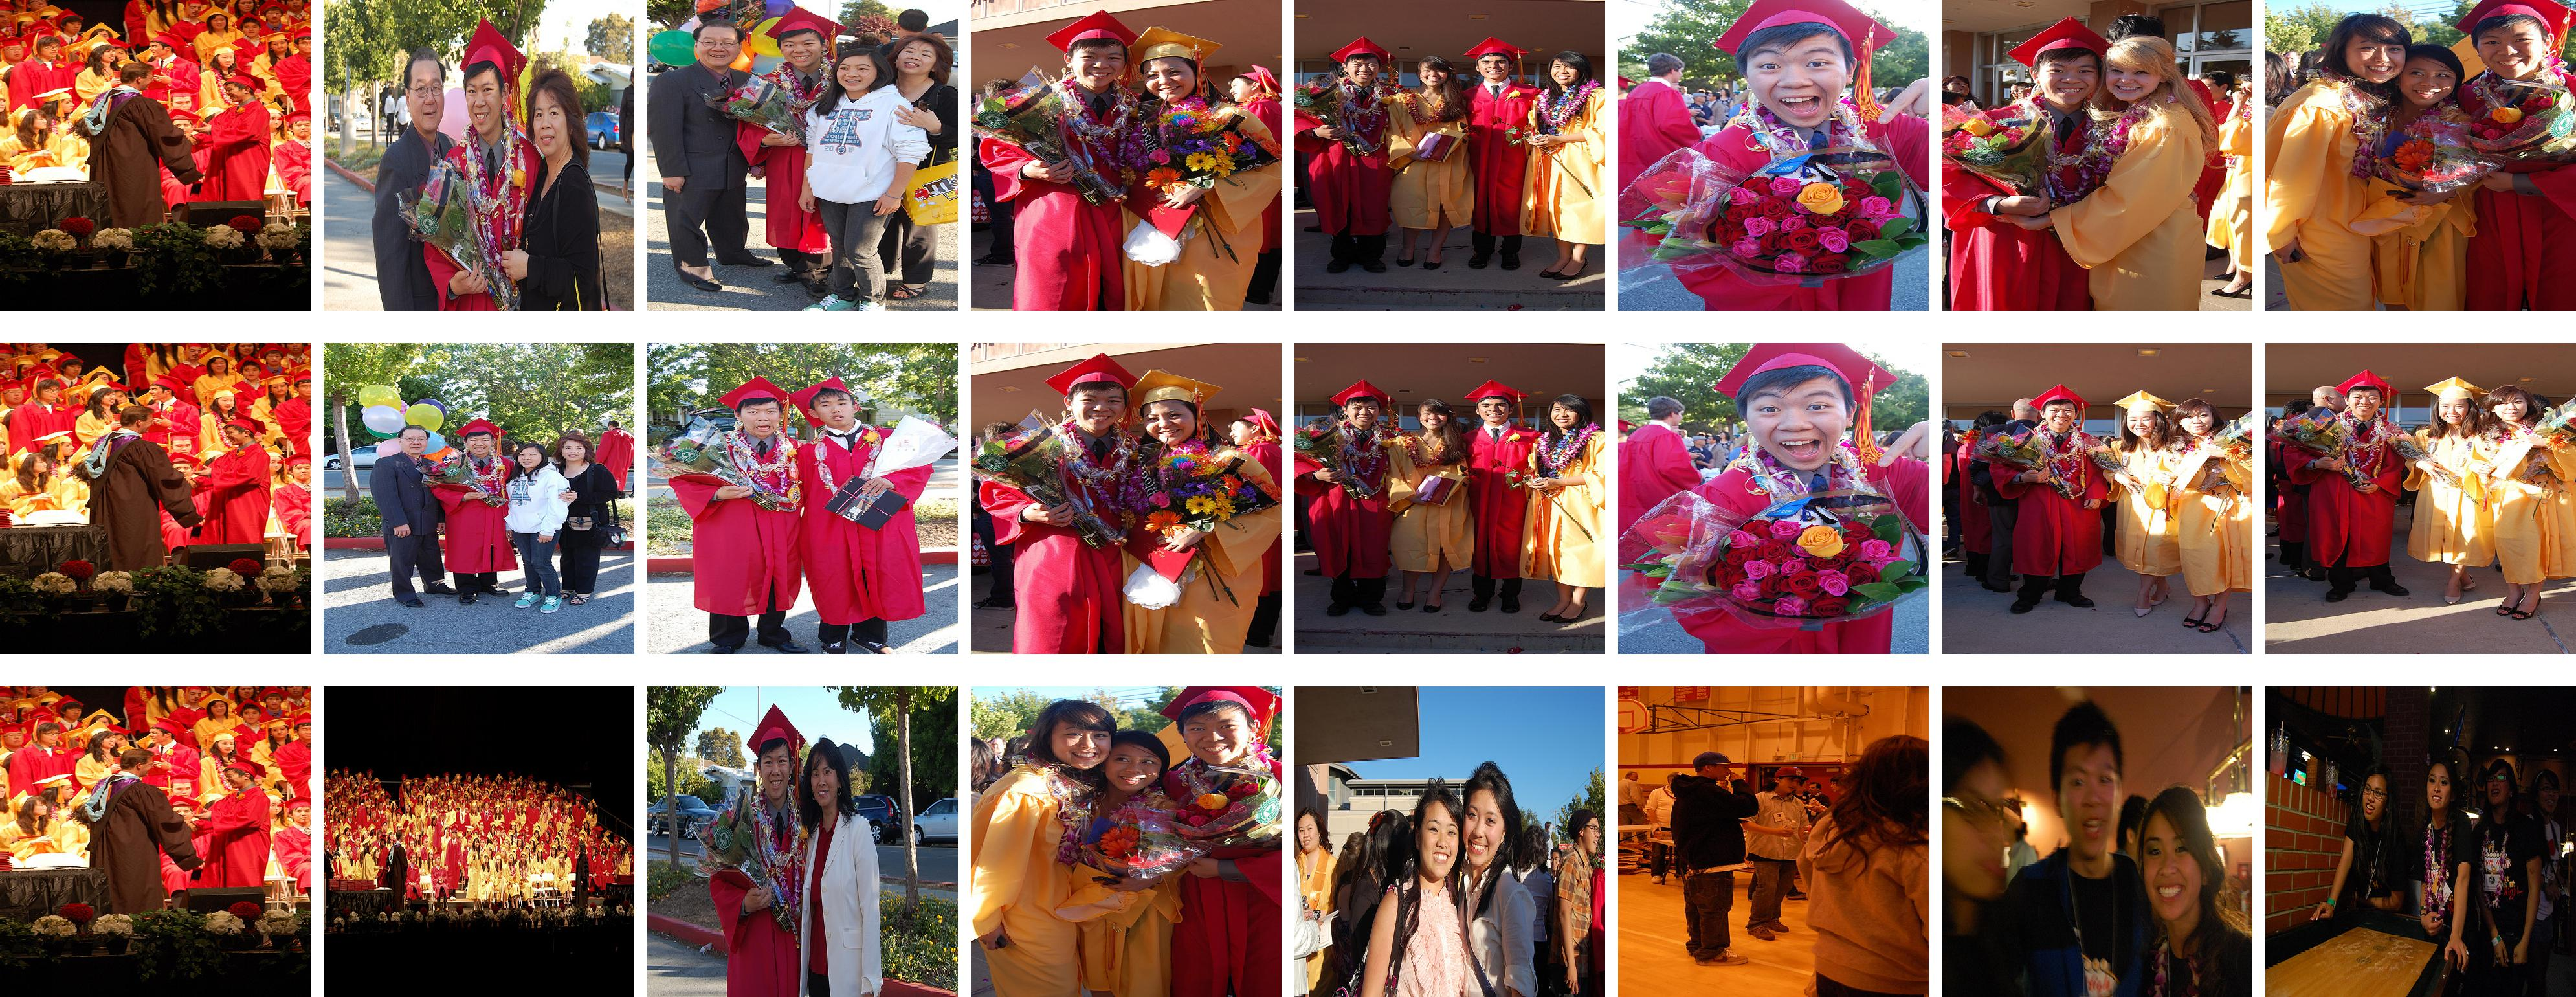
\includegraphics[height=1.5in]{results/a3_0_12356498@N06_8_10.jpg}}
  \subcaptionbox{Top 15\% of a \textit{Personal Sports} album. \label{fig14}}{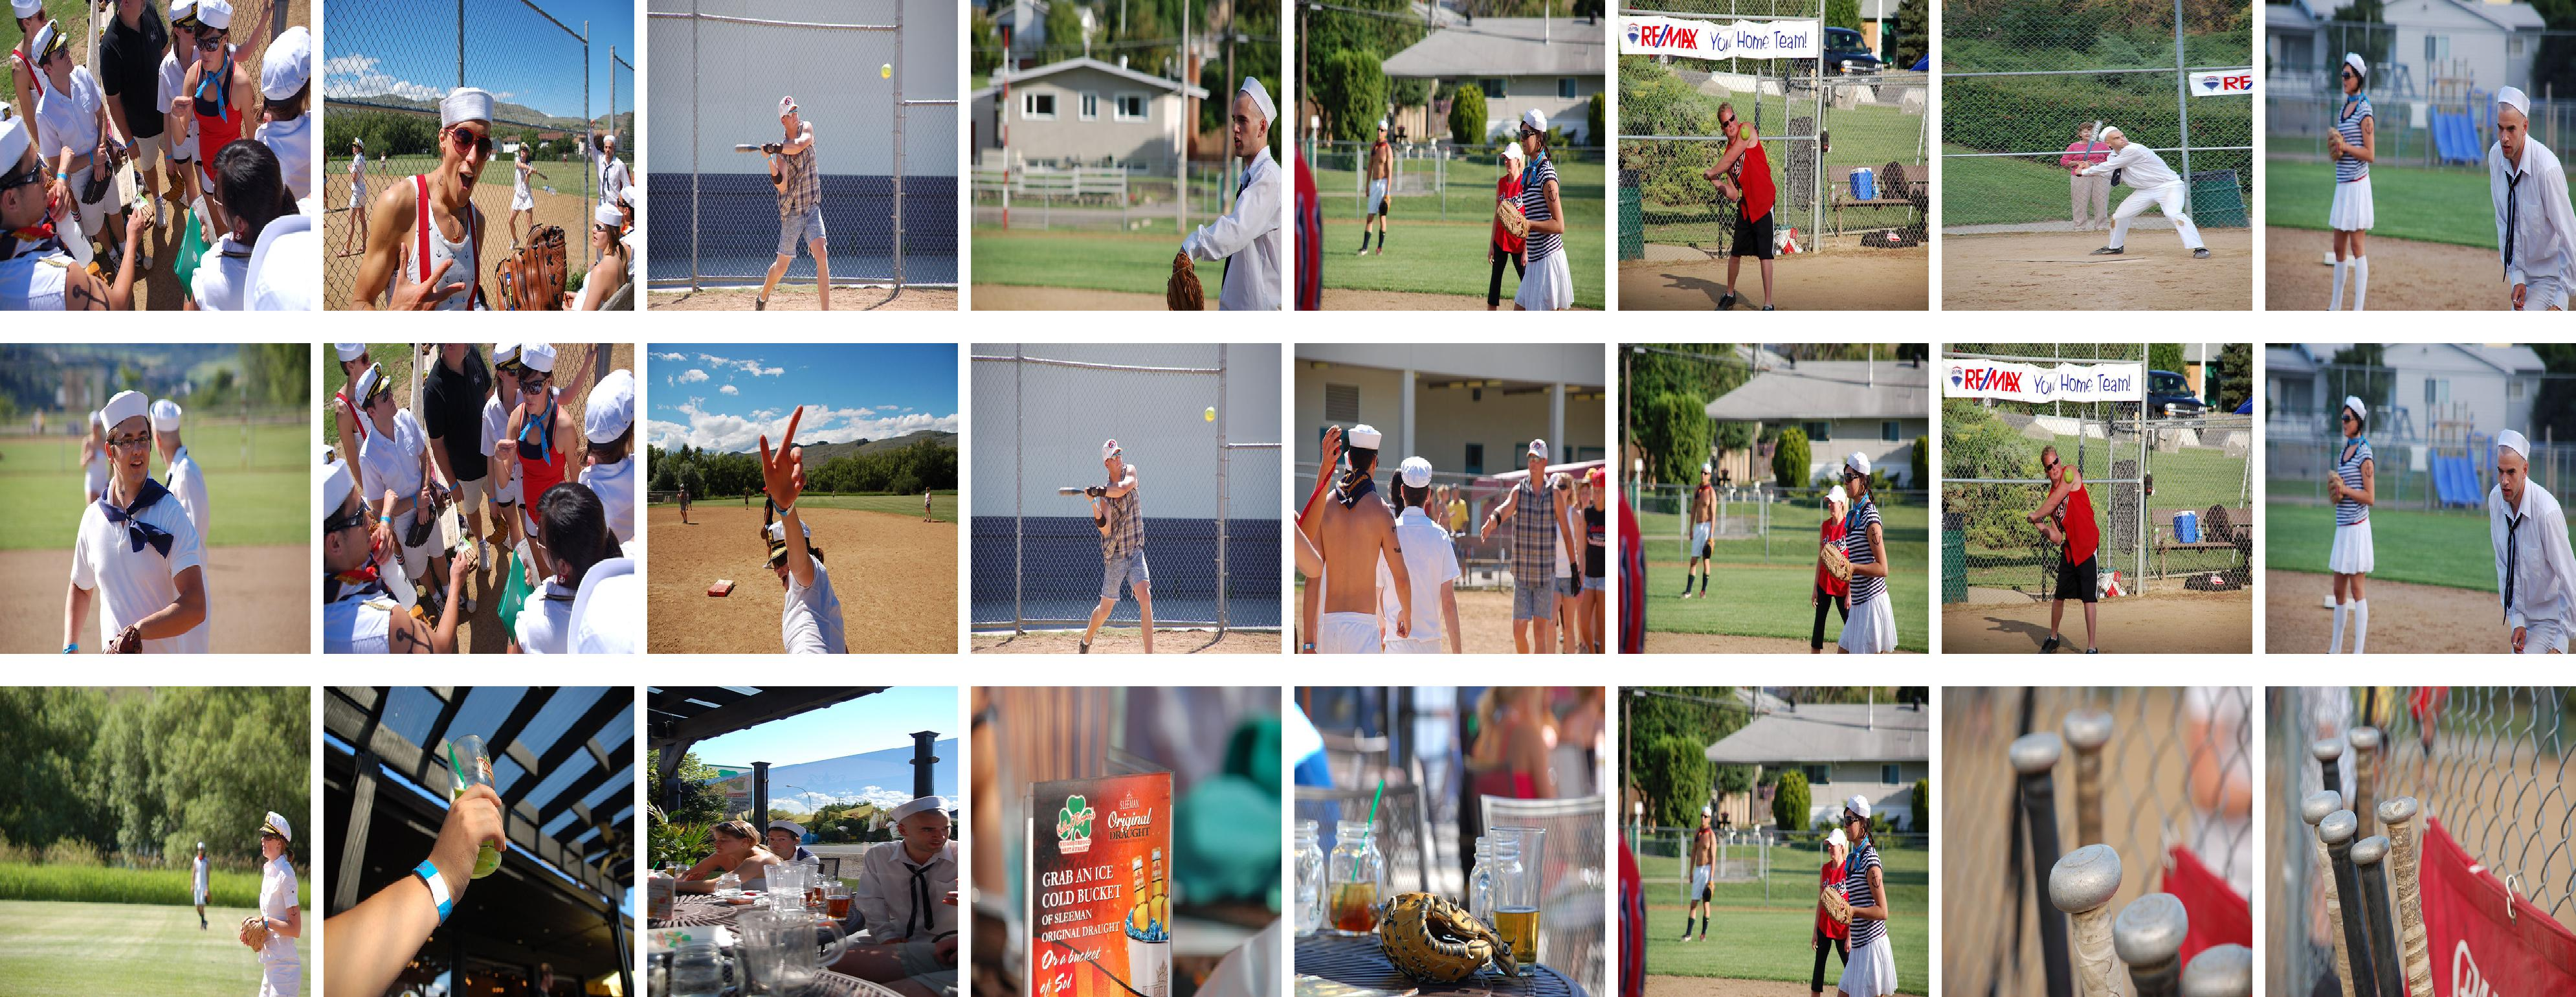
\includegraphics[height=1.5in]{results/a4_0_70644035@N00_8_15.jpg}}
  \subcaptionbox{Top 20\% of a \textit{Birthday} album. \label{fig15}}{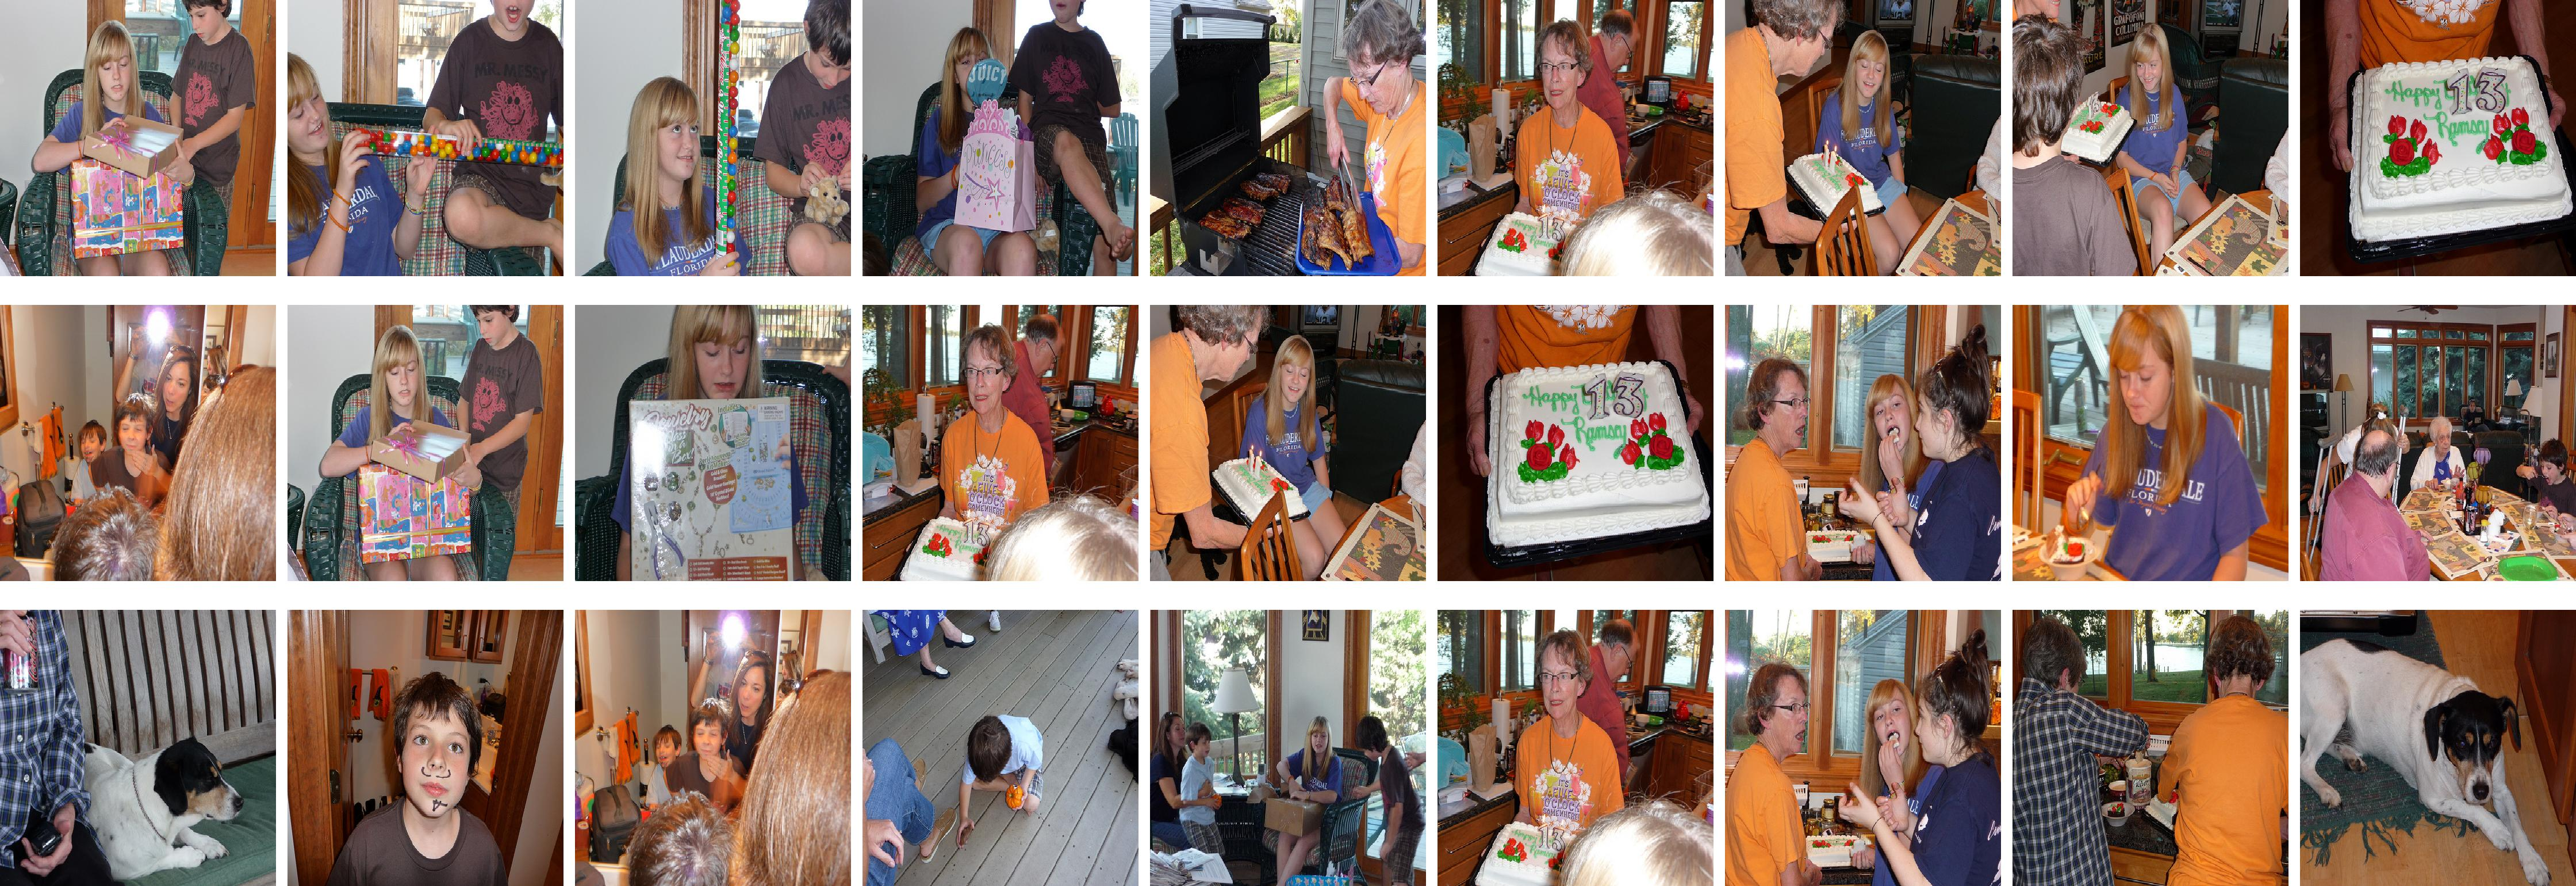
\includegraphics[height=1.5in]{results/a5_0_28004076@N04_9_20.jpg}}
  \end{figure*}
  
\clearpage
  \begin{figure*}[ht]
\ContinuedFloat % continue from previous page
\centering
  \subcaptionbox{Top 20\% of a \textit{Halloween} album. \label{fig16}}{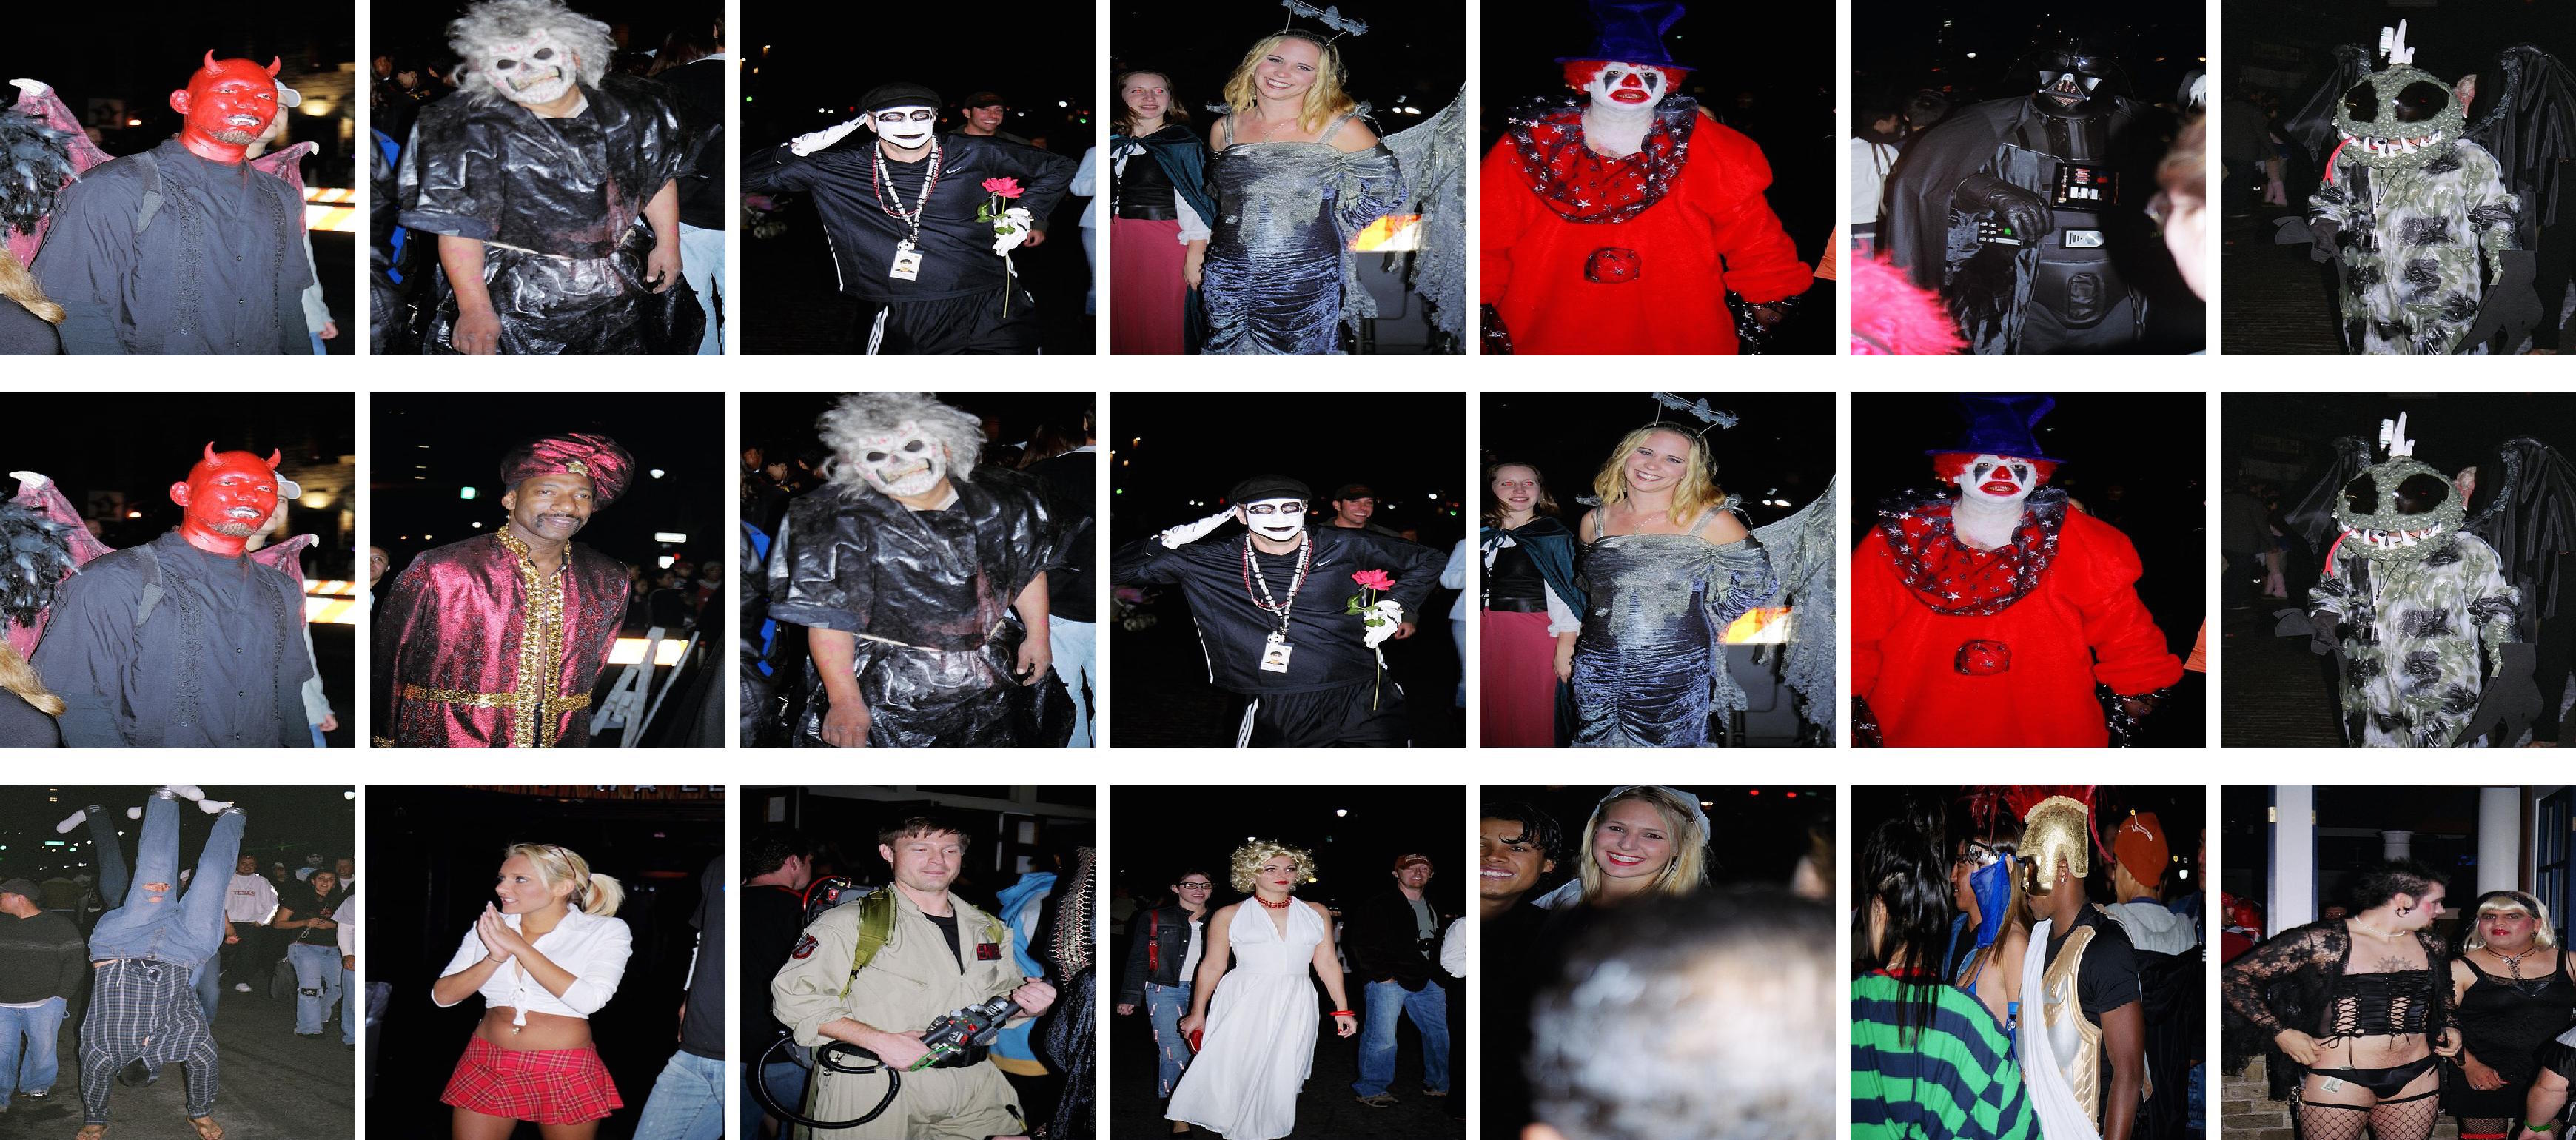
\includegraphics[height=1.5in]{results/new_0_57185608@N00_7_20.jpg}} \hspace{2em}
    \subcaptionbox{Top 20\% of a \textit{Personal Sports} album. \label{fig17}}{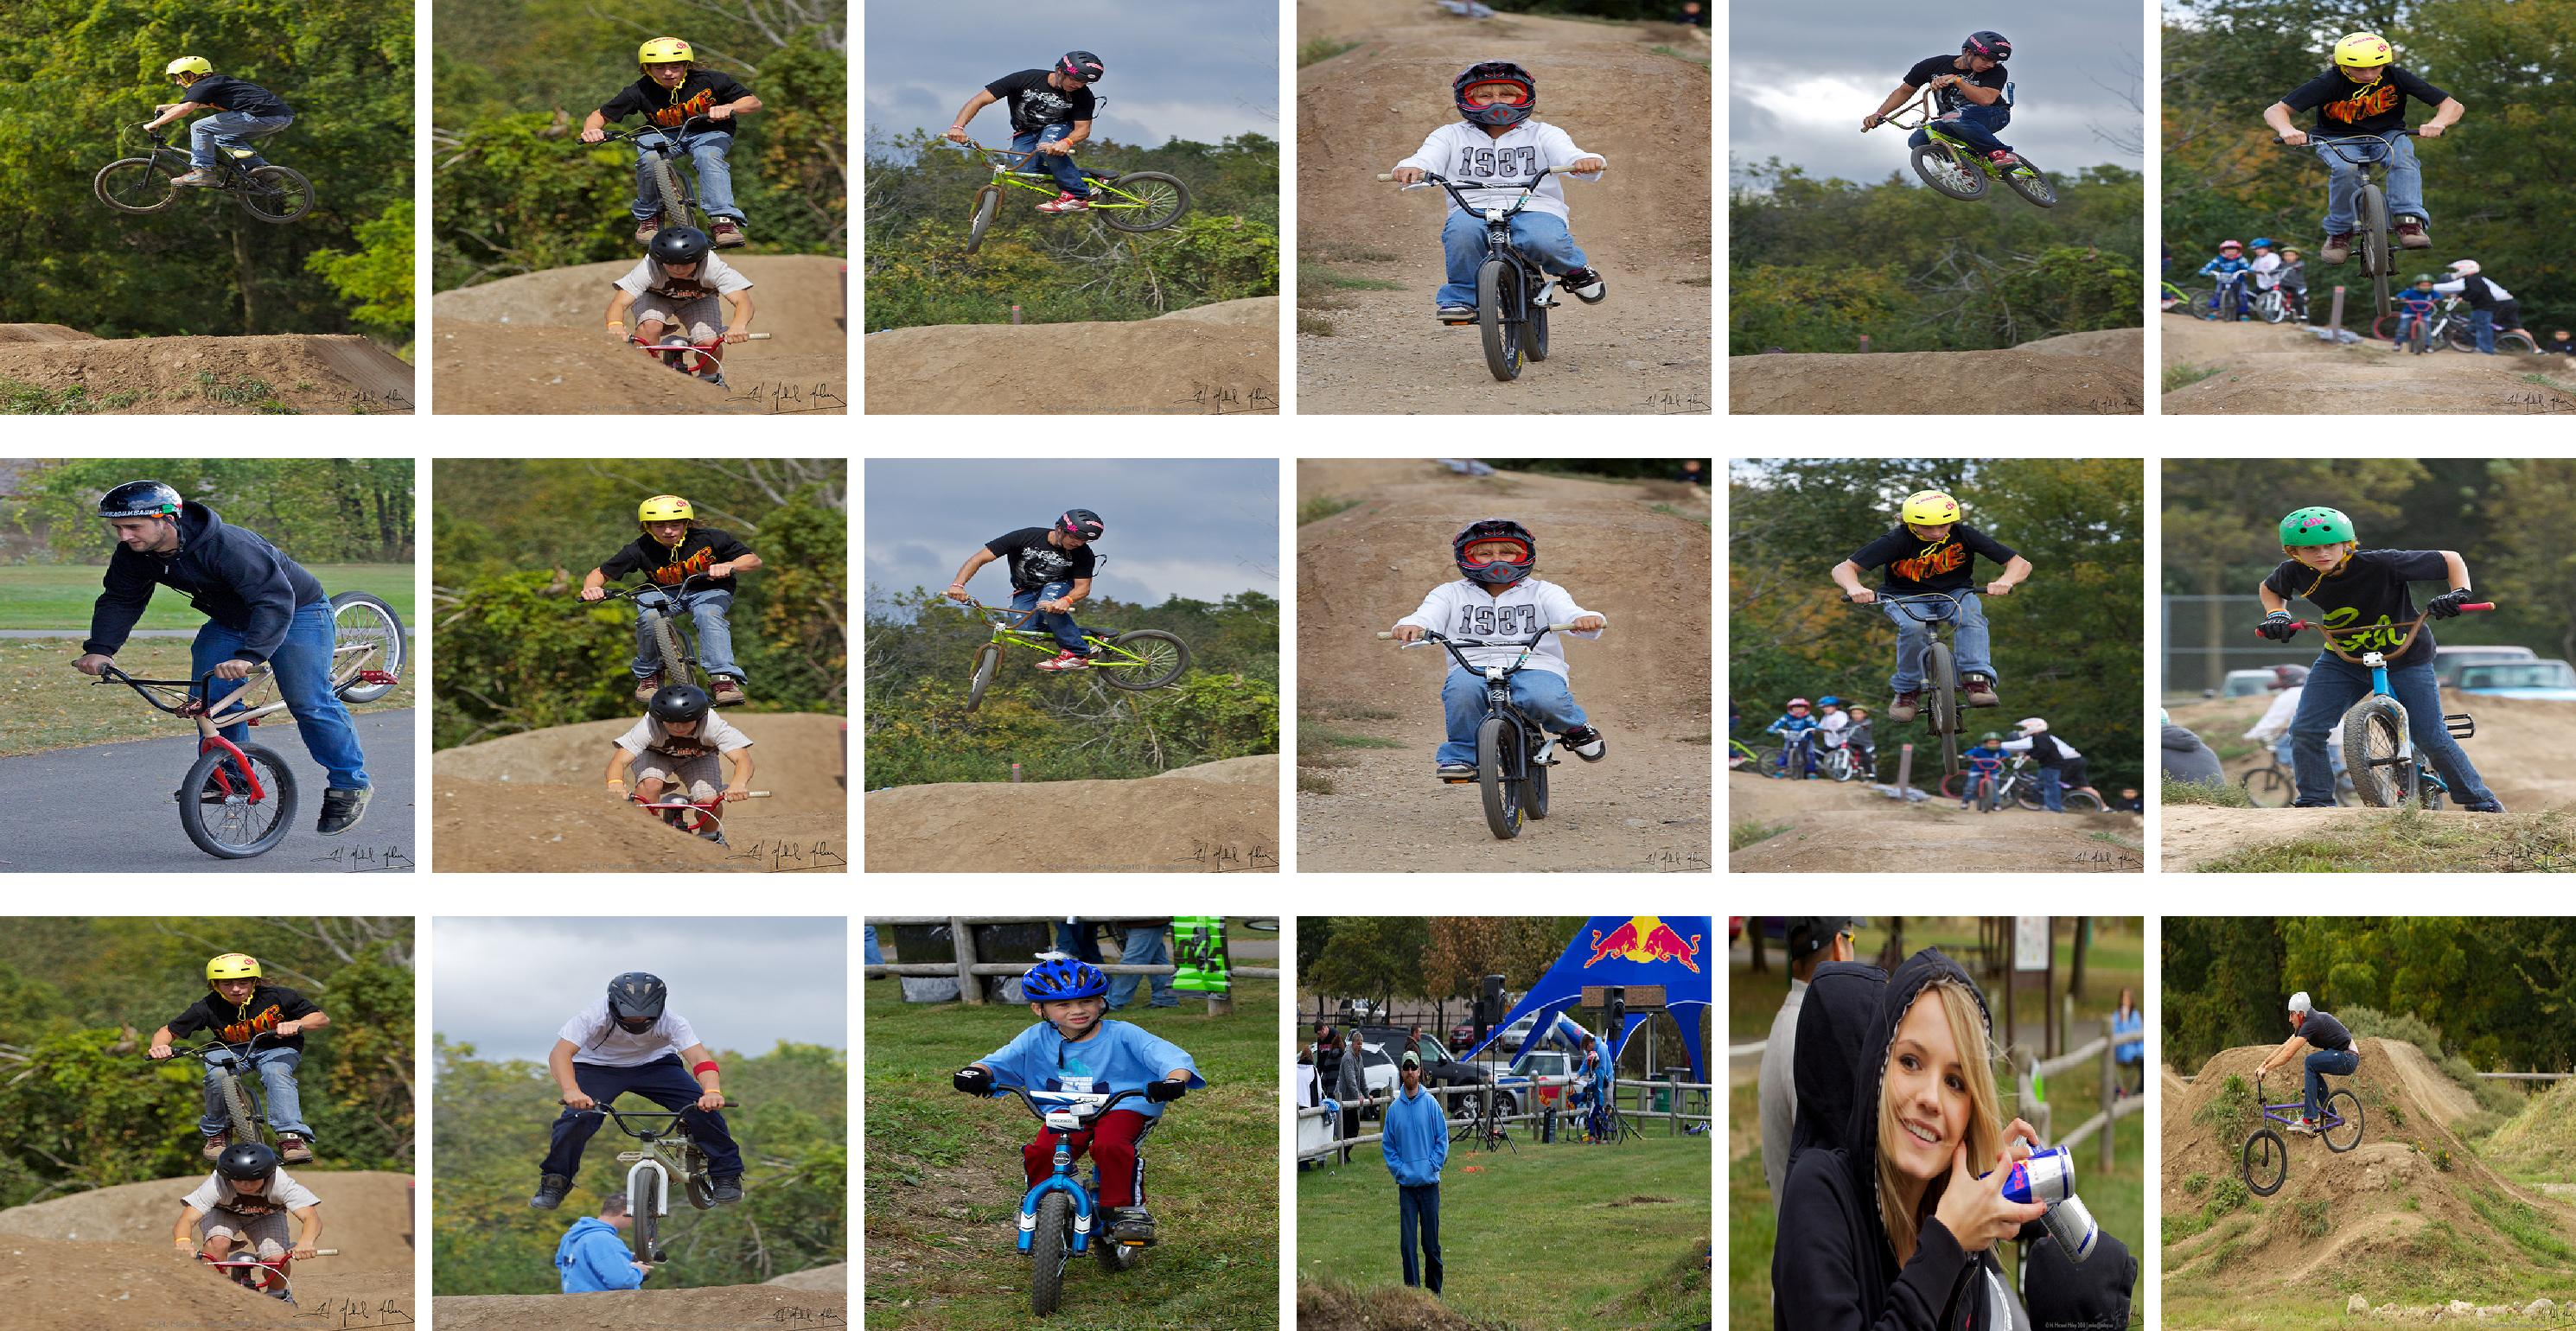
\includegraphics[height=1.5in]{results/a7_40_44082489@N00_6_20.jpg}} 
  \subcaptionbox{Top 20\% of a \textit{Show} album. \label{fig18}}{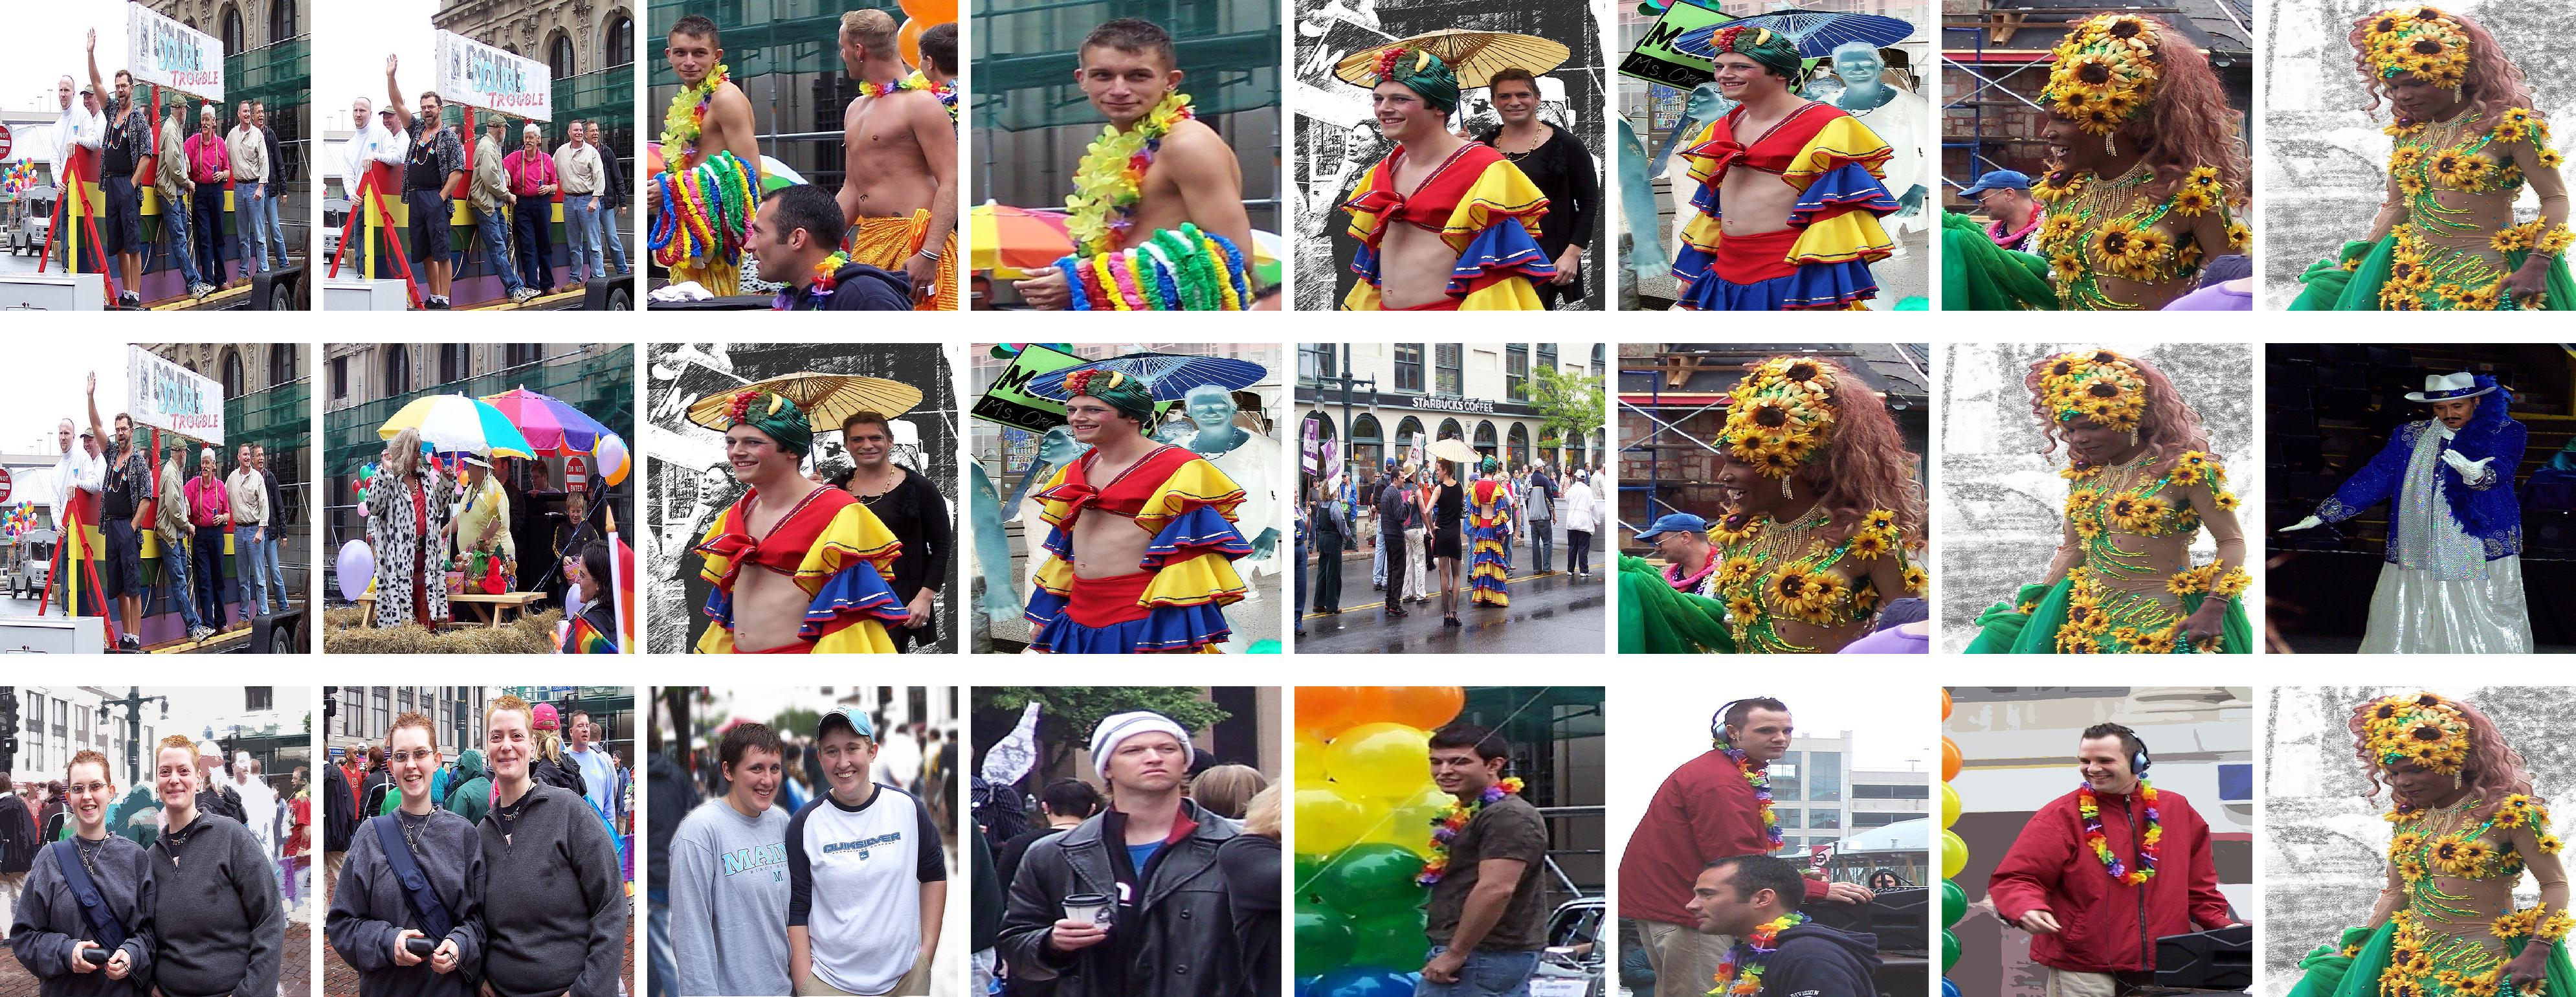
\includegraphics[height=1.5in]{results/a8_0_70054695@N00_8_20.jpg}} \\
  \subcaptionbox{Top 20\% of a \textit{Sports} album. \label{fig19}}{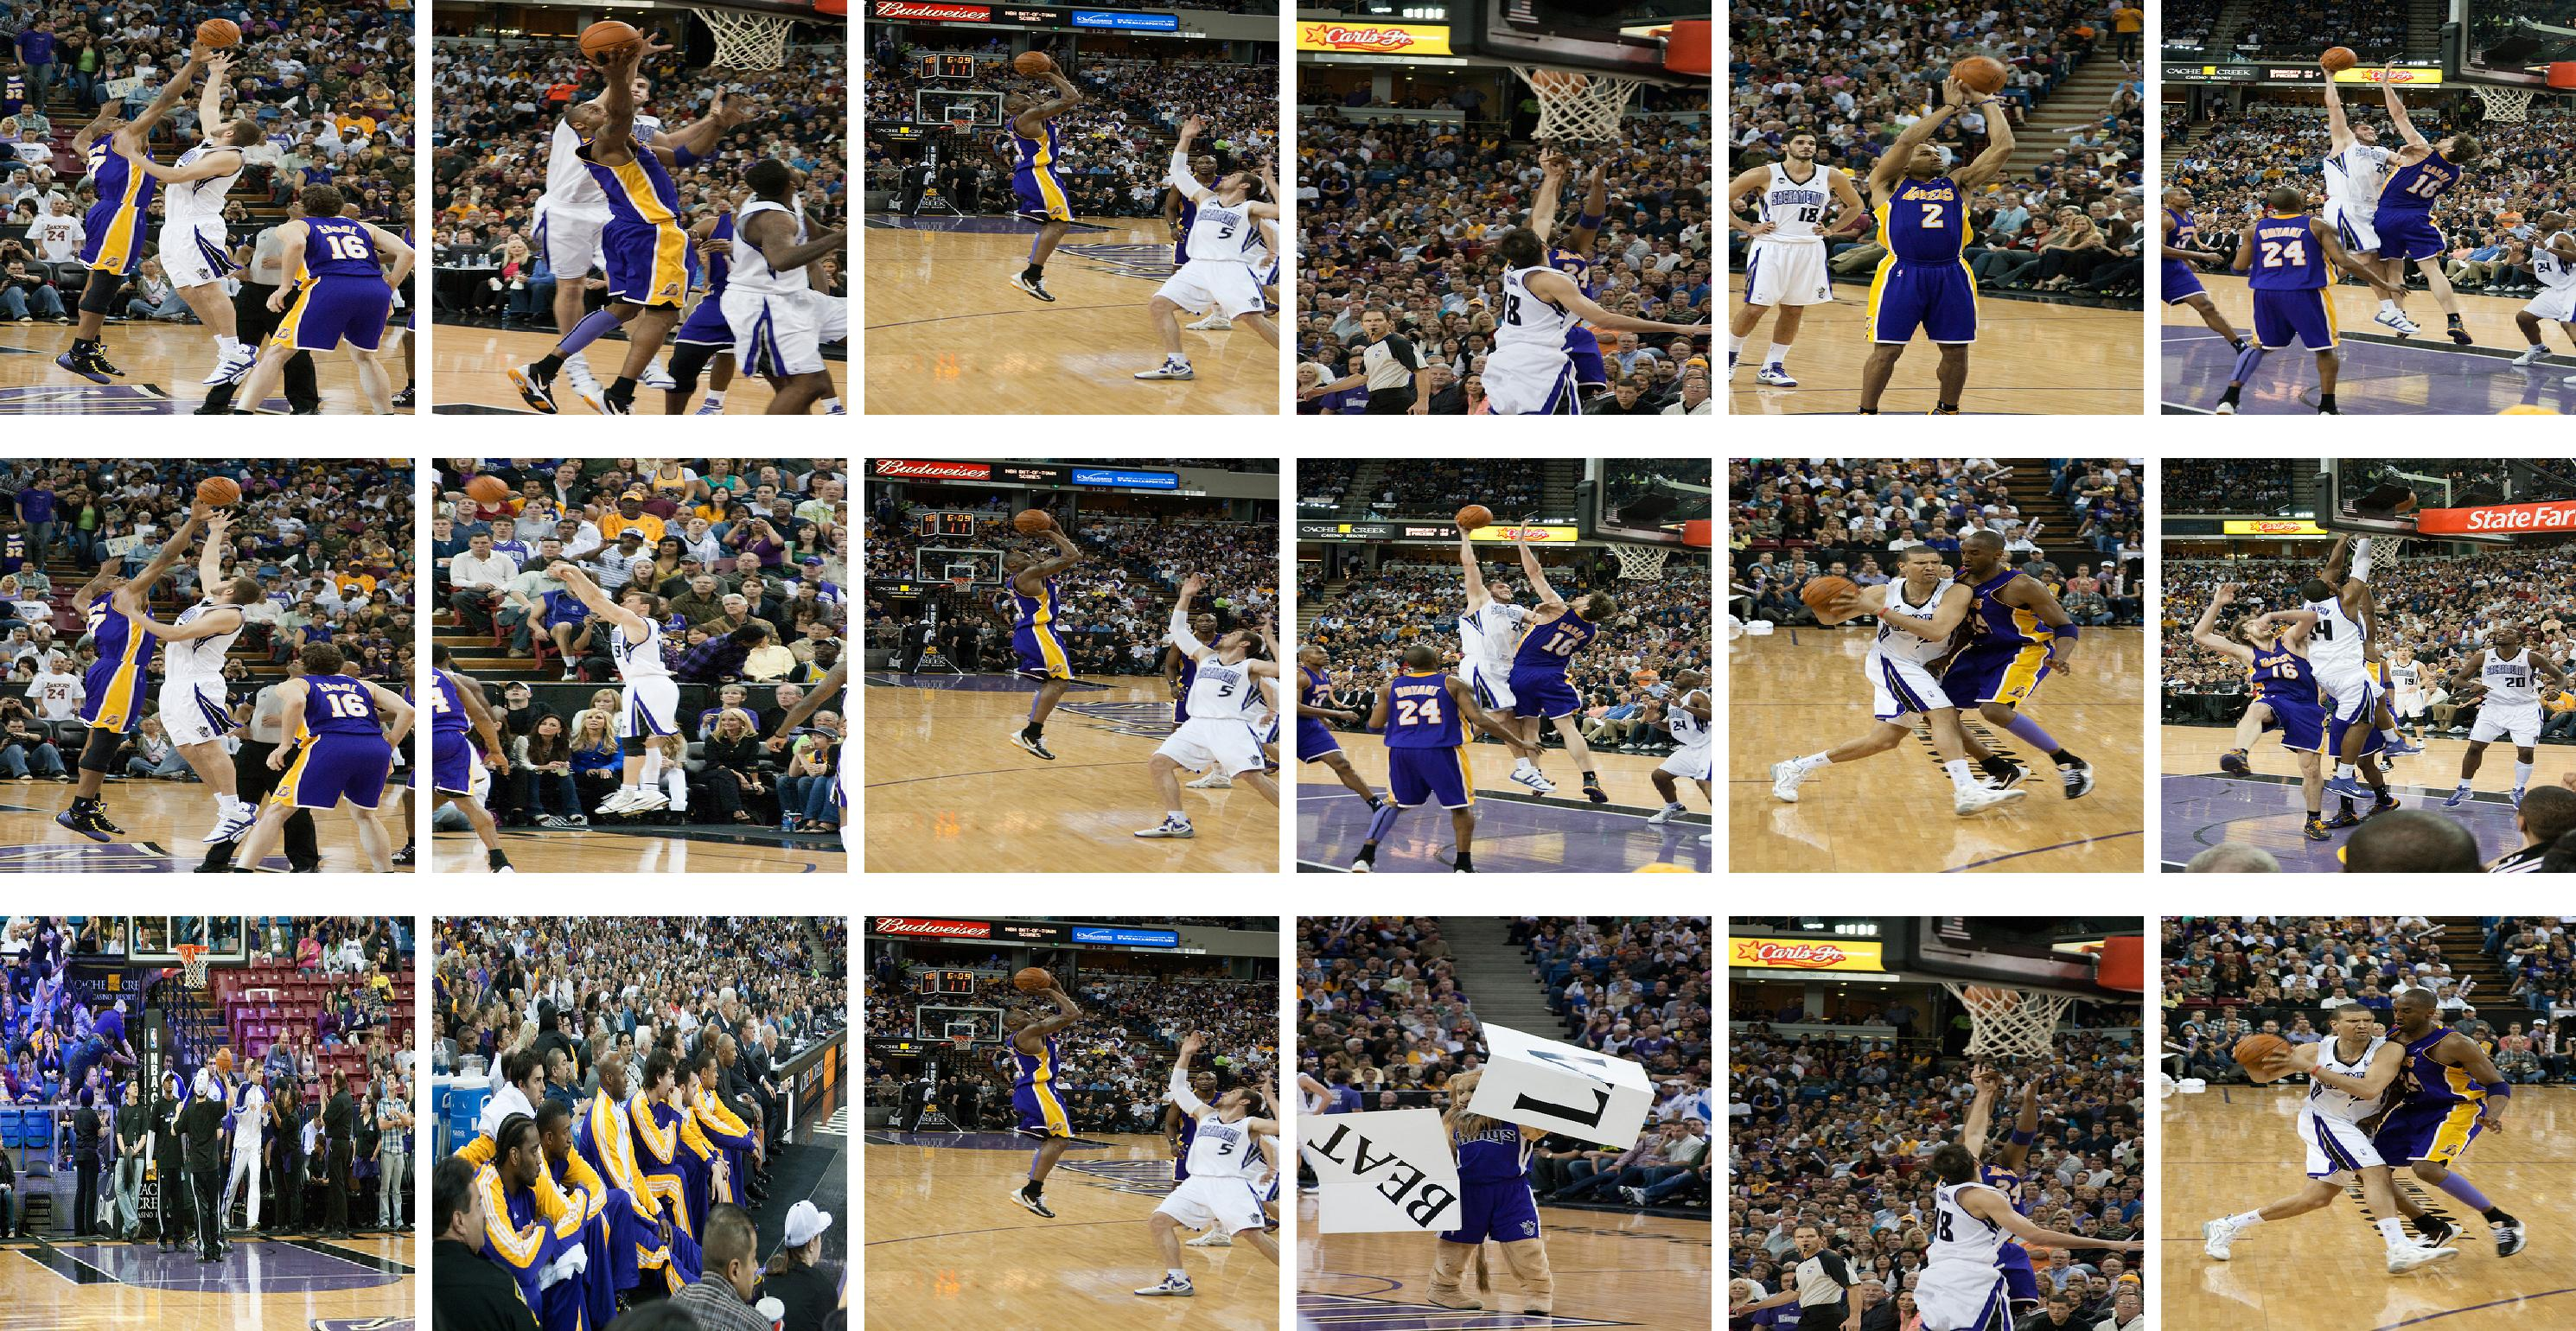
\includegraphics[height=1.5in]{results/a9_0_51517883@N00_6_20.jpg}} \hspace{2em}
  \subcaptionbox{Top 20\% of a \textit{Personal Music Activity} album. \label{fig20}}{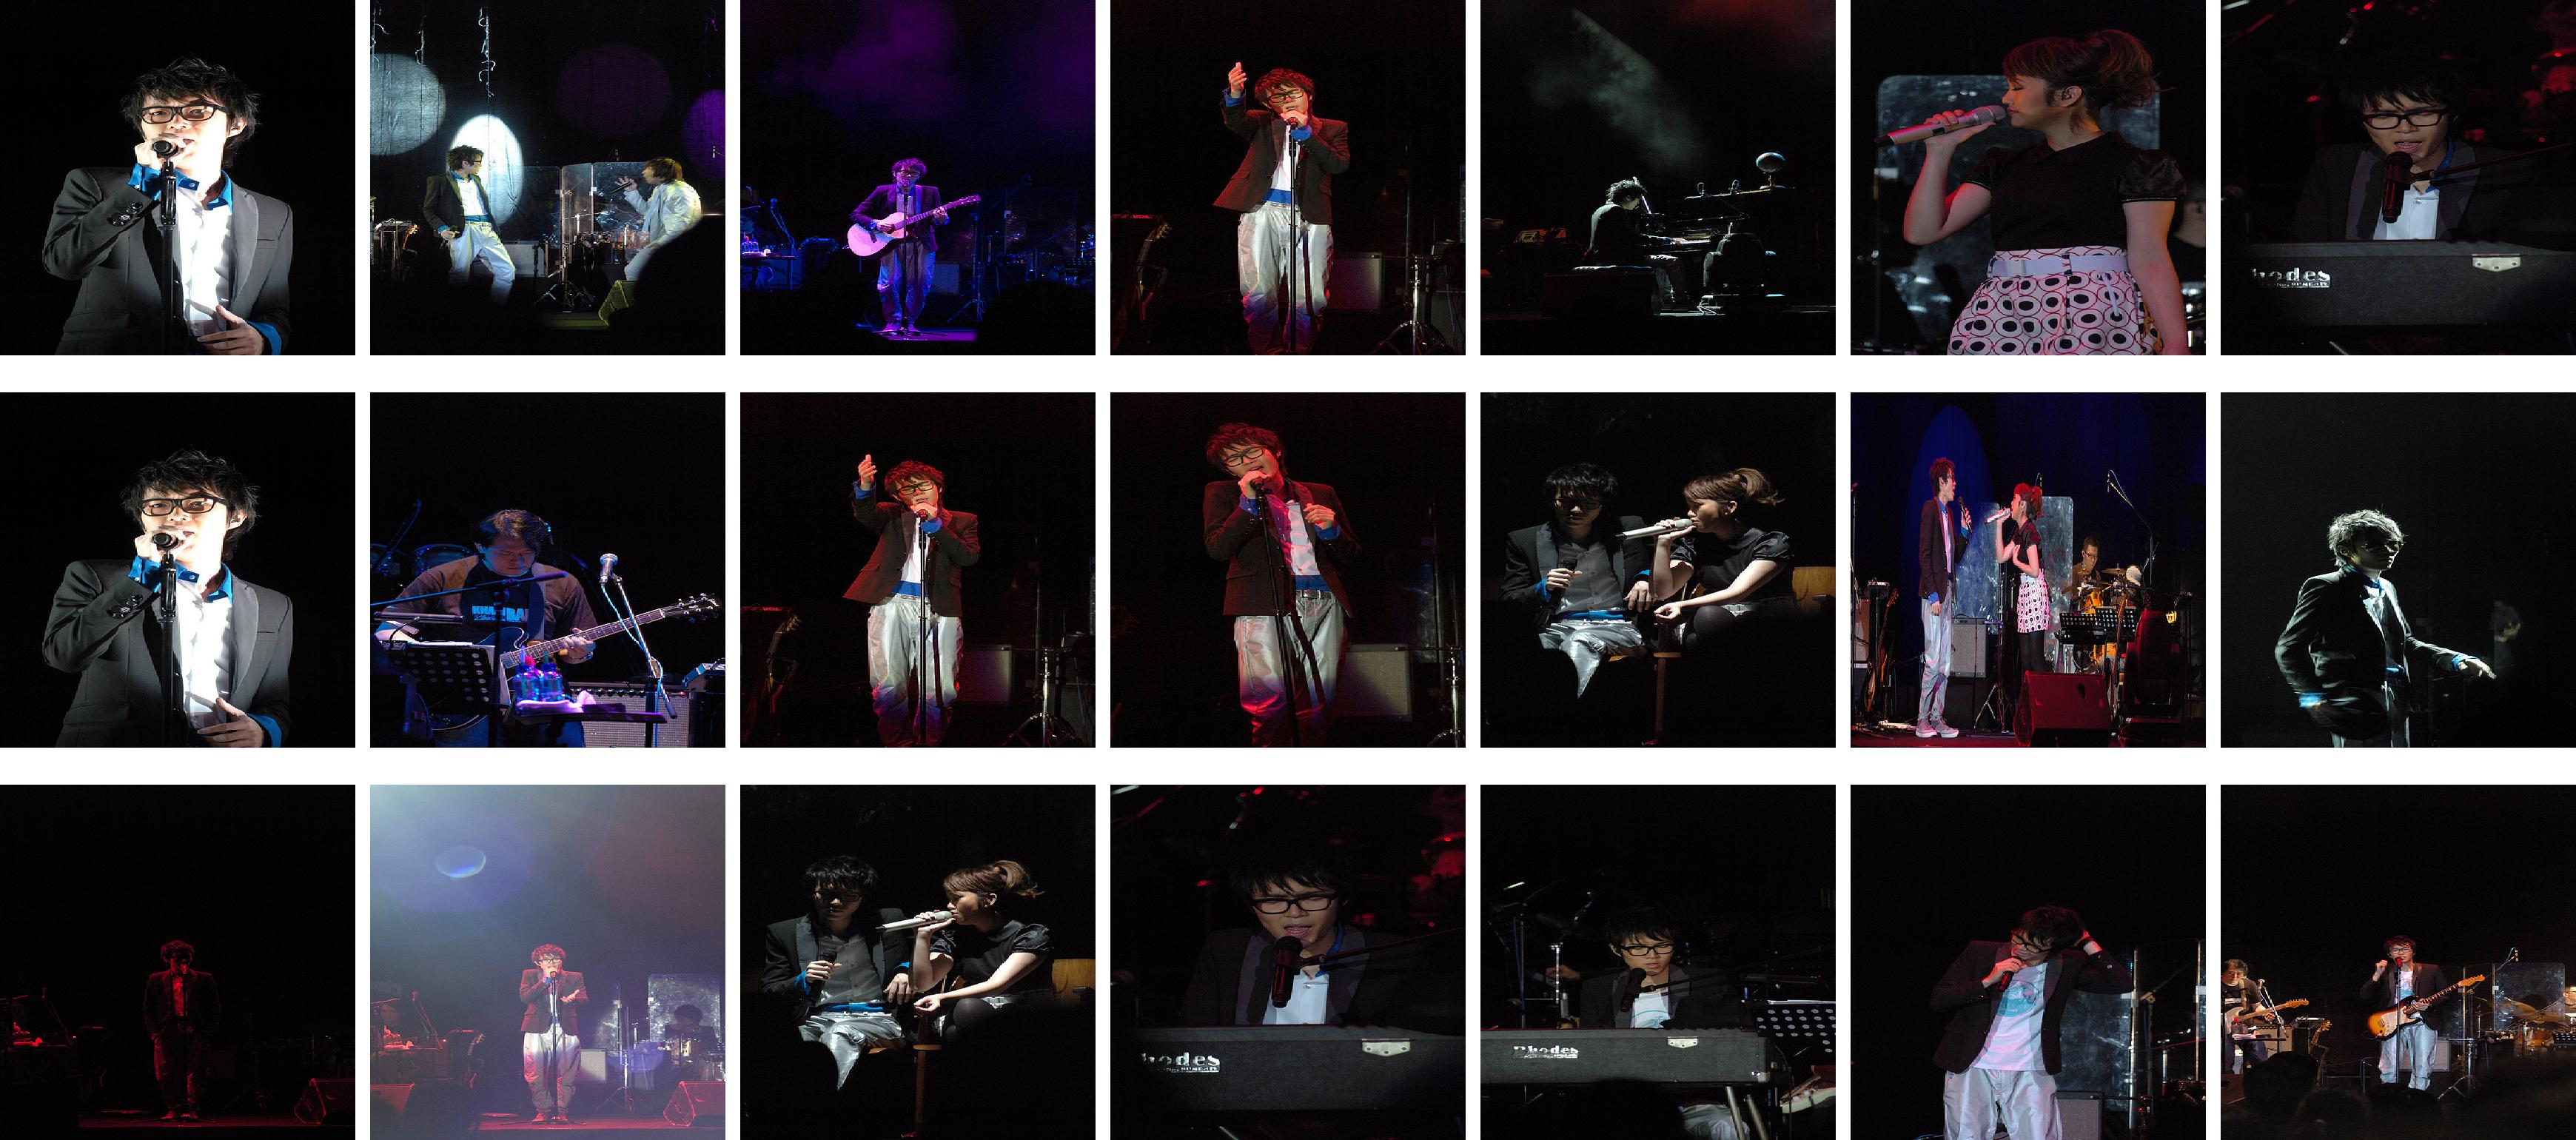
\includegraphics[height=1.5in]{results/a10_0_52685047@N00_7_20.jpg}}
  \subcaptionbox{Top 20\% of a \textit{Theme Park} album. \label{fig21}}{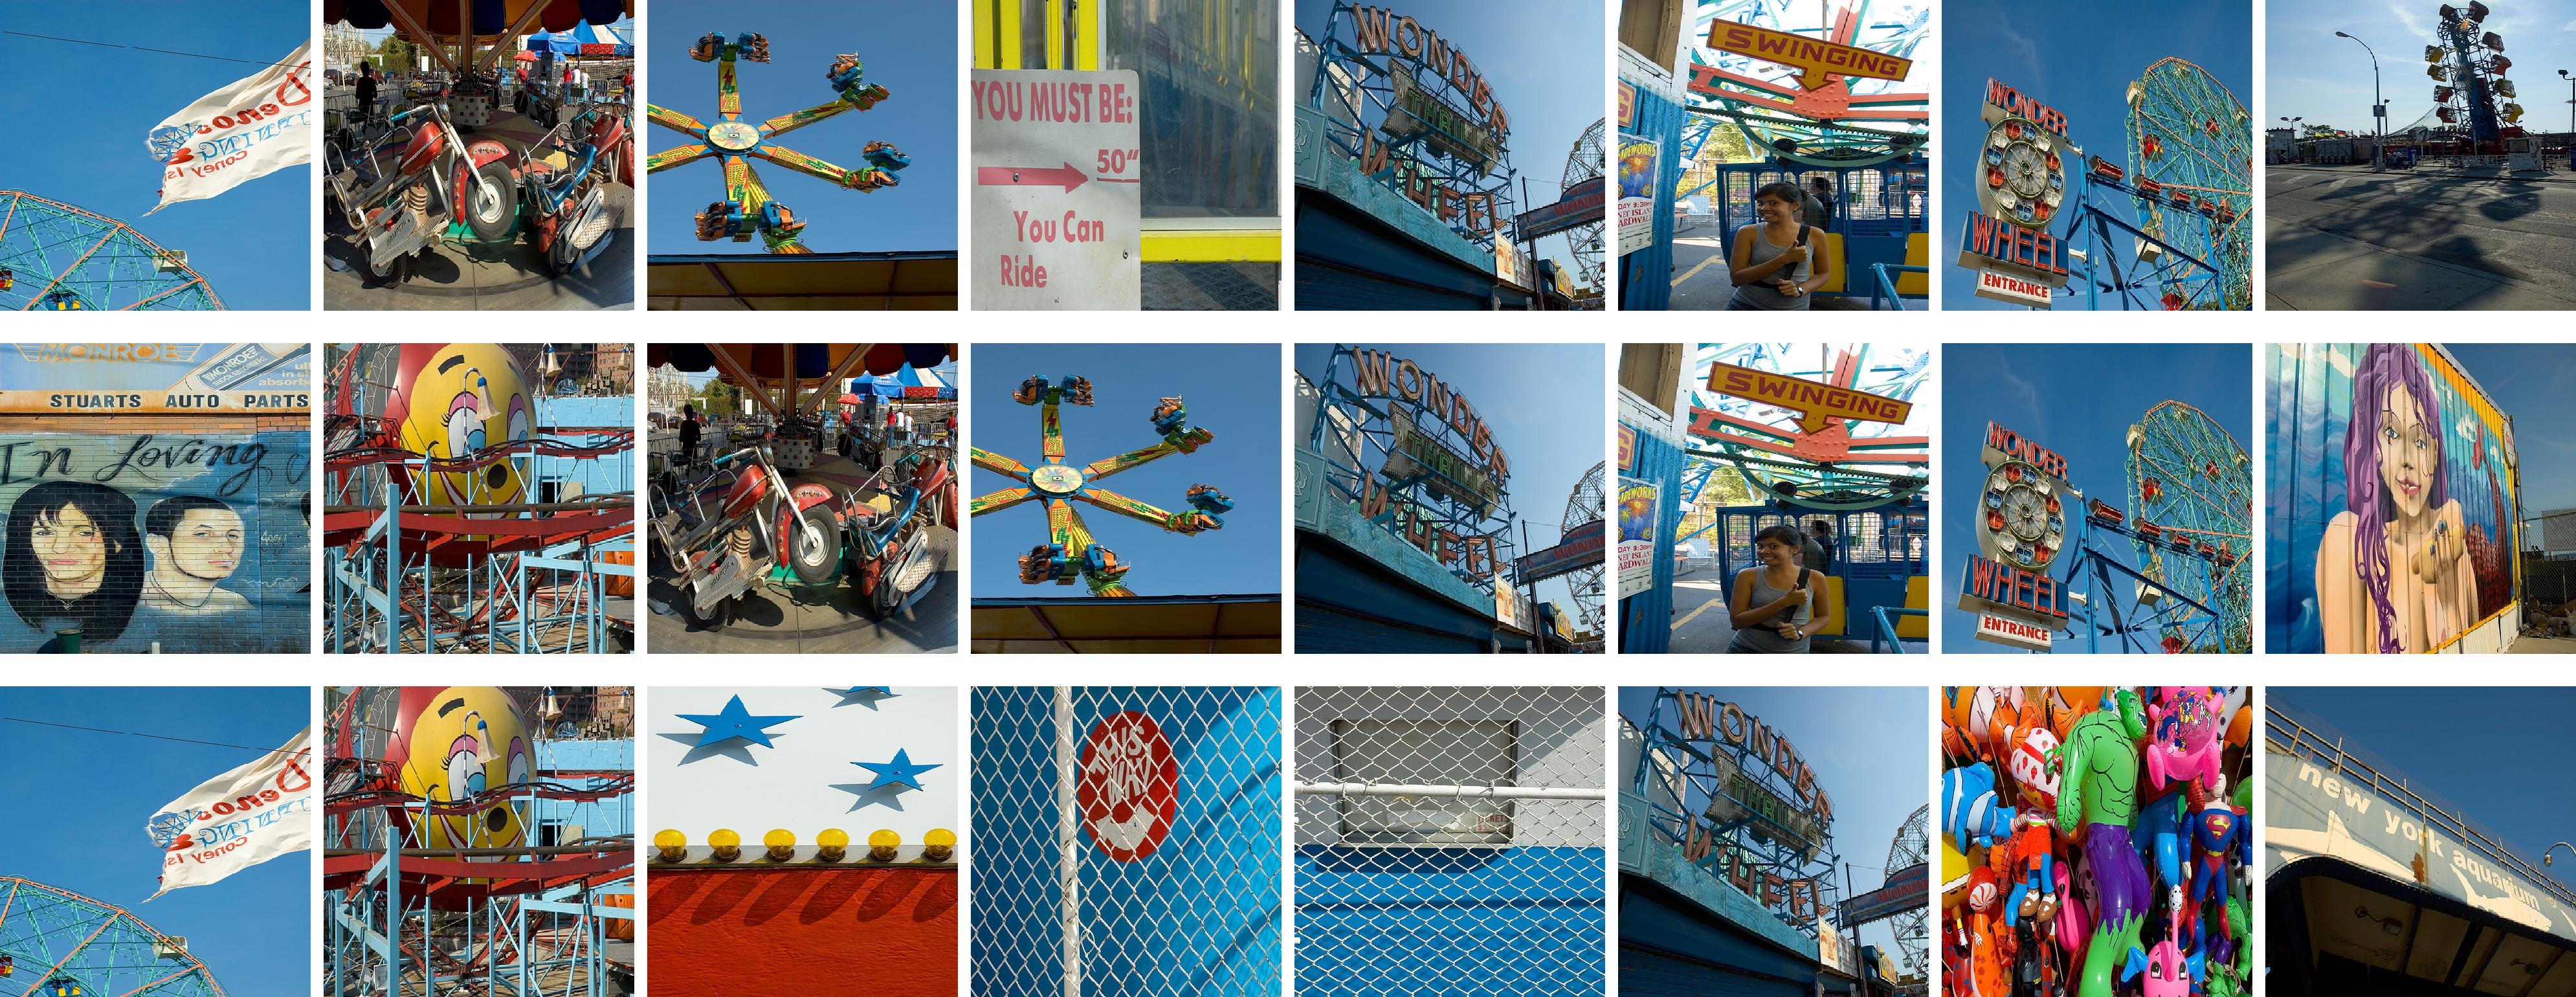
\includegraphics[height=1.5in]{results/a11_37_30952578@N00_8_20.jpg}}
  \subcaptionbox{Top 10\% of a \textit{Halloween} album. \label{fig22}}{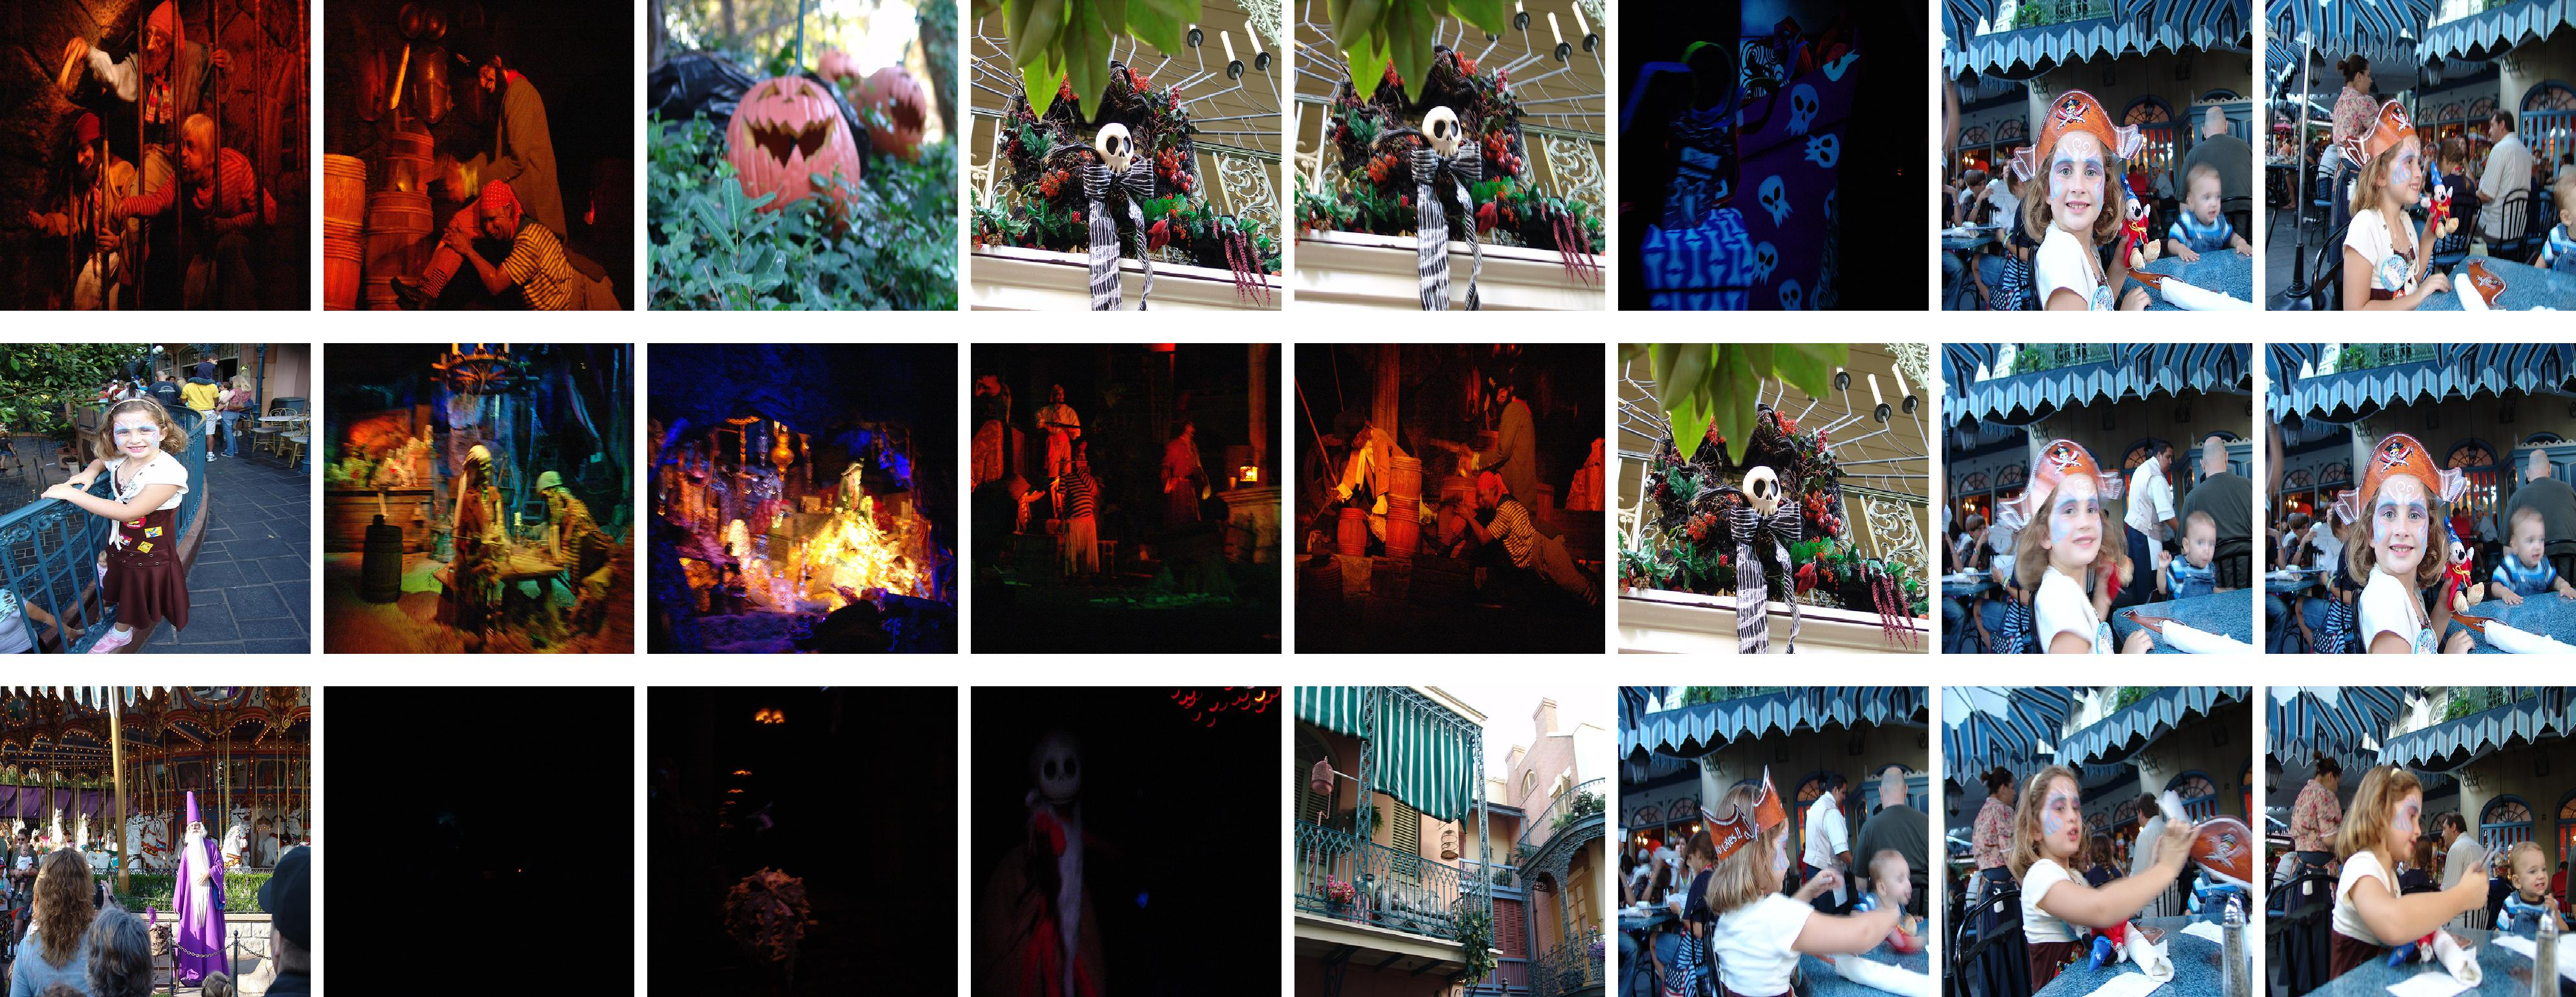
\includegraphics[height=1.5in]{results/a12_0_40958113@N00_8_10.jpg}}
    \end{figure*}
  
\clearpage
  \begin{figure*}[ht]
  \ContinuedFloat % continue from previous page
\centering
  \subcaptionbox{Top 20\% of a \textit{Wedding} album. \label{fig23}}{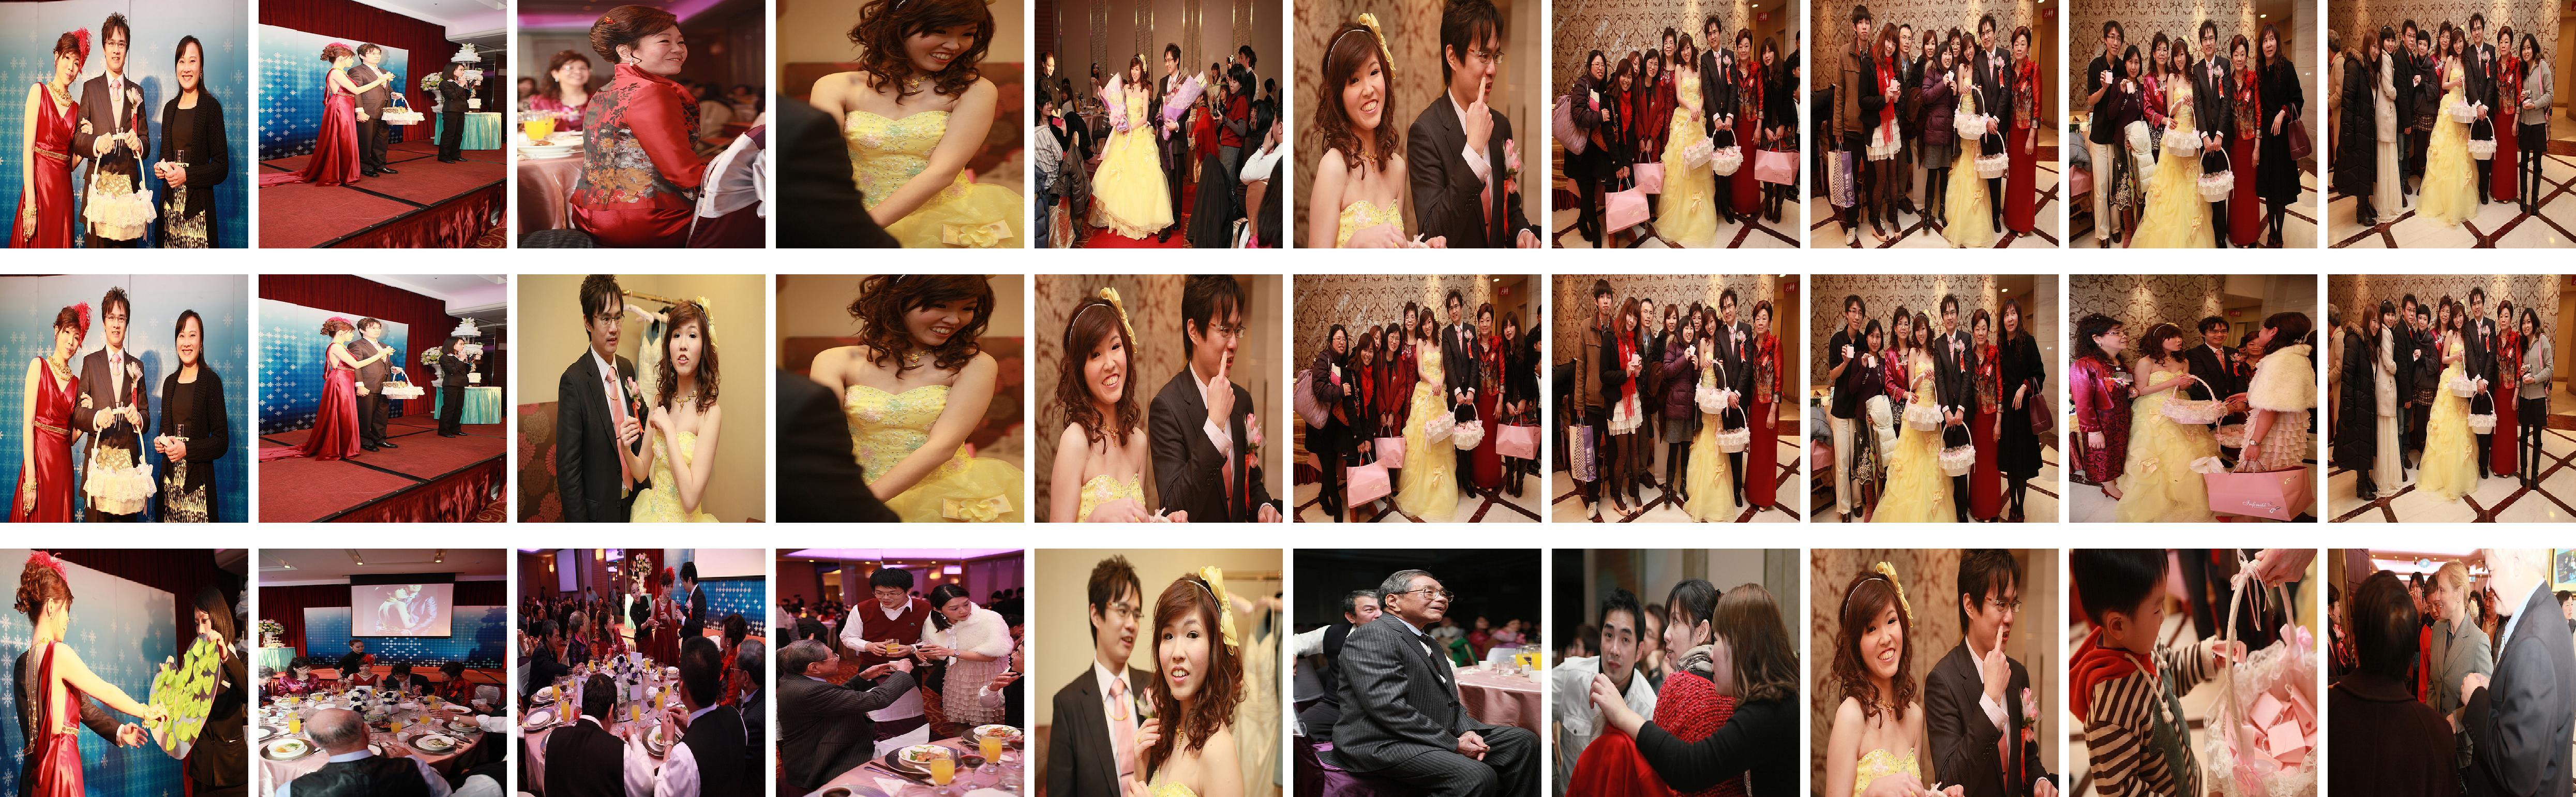
\includegraphics[height=1.5in]{results/a13_1_51164183@N07_10_20.jpg}}
  \subcaptionbox{Top 15\% of a \textit{Cruise Trip} album. \label{fig24}}{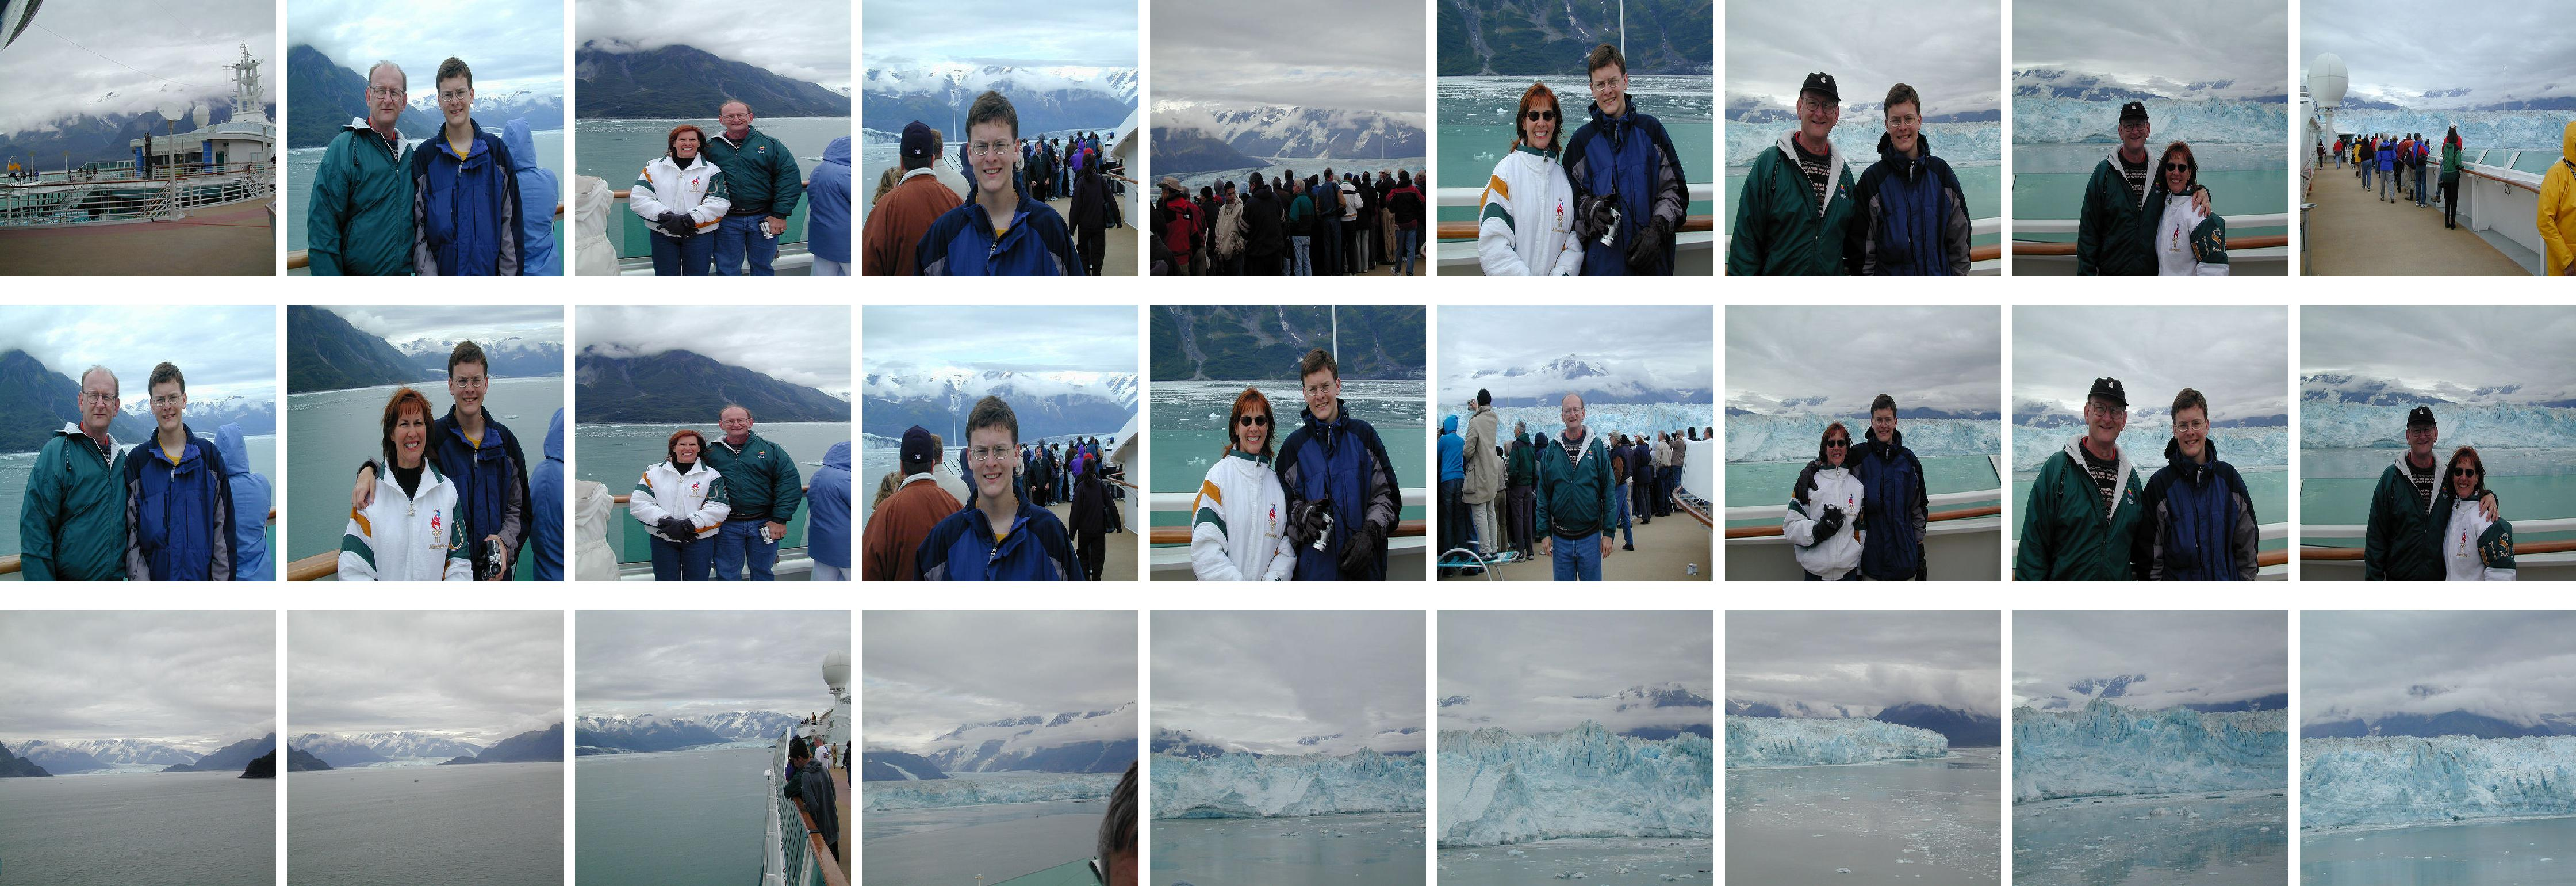
\includegraphics[height=1.5in]{results/a14_1_56922885@N00_9_15.jpg}}
  \subcaptionbox{Top 20\% of a \textit{Wedding} album. \label{fig25}}{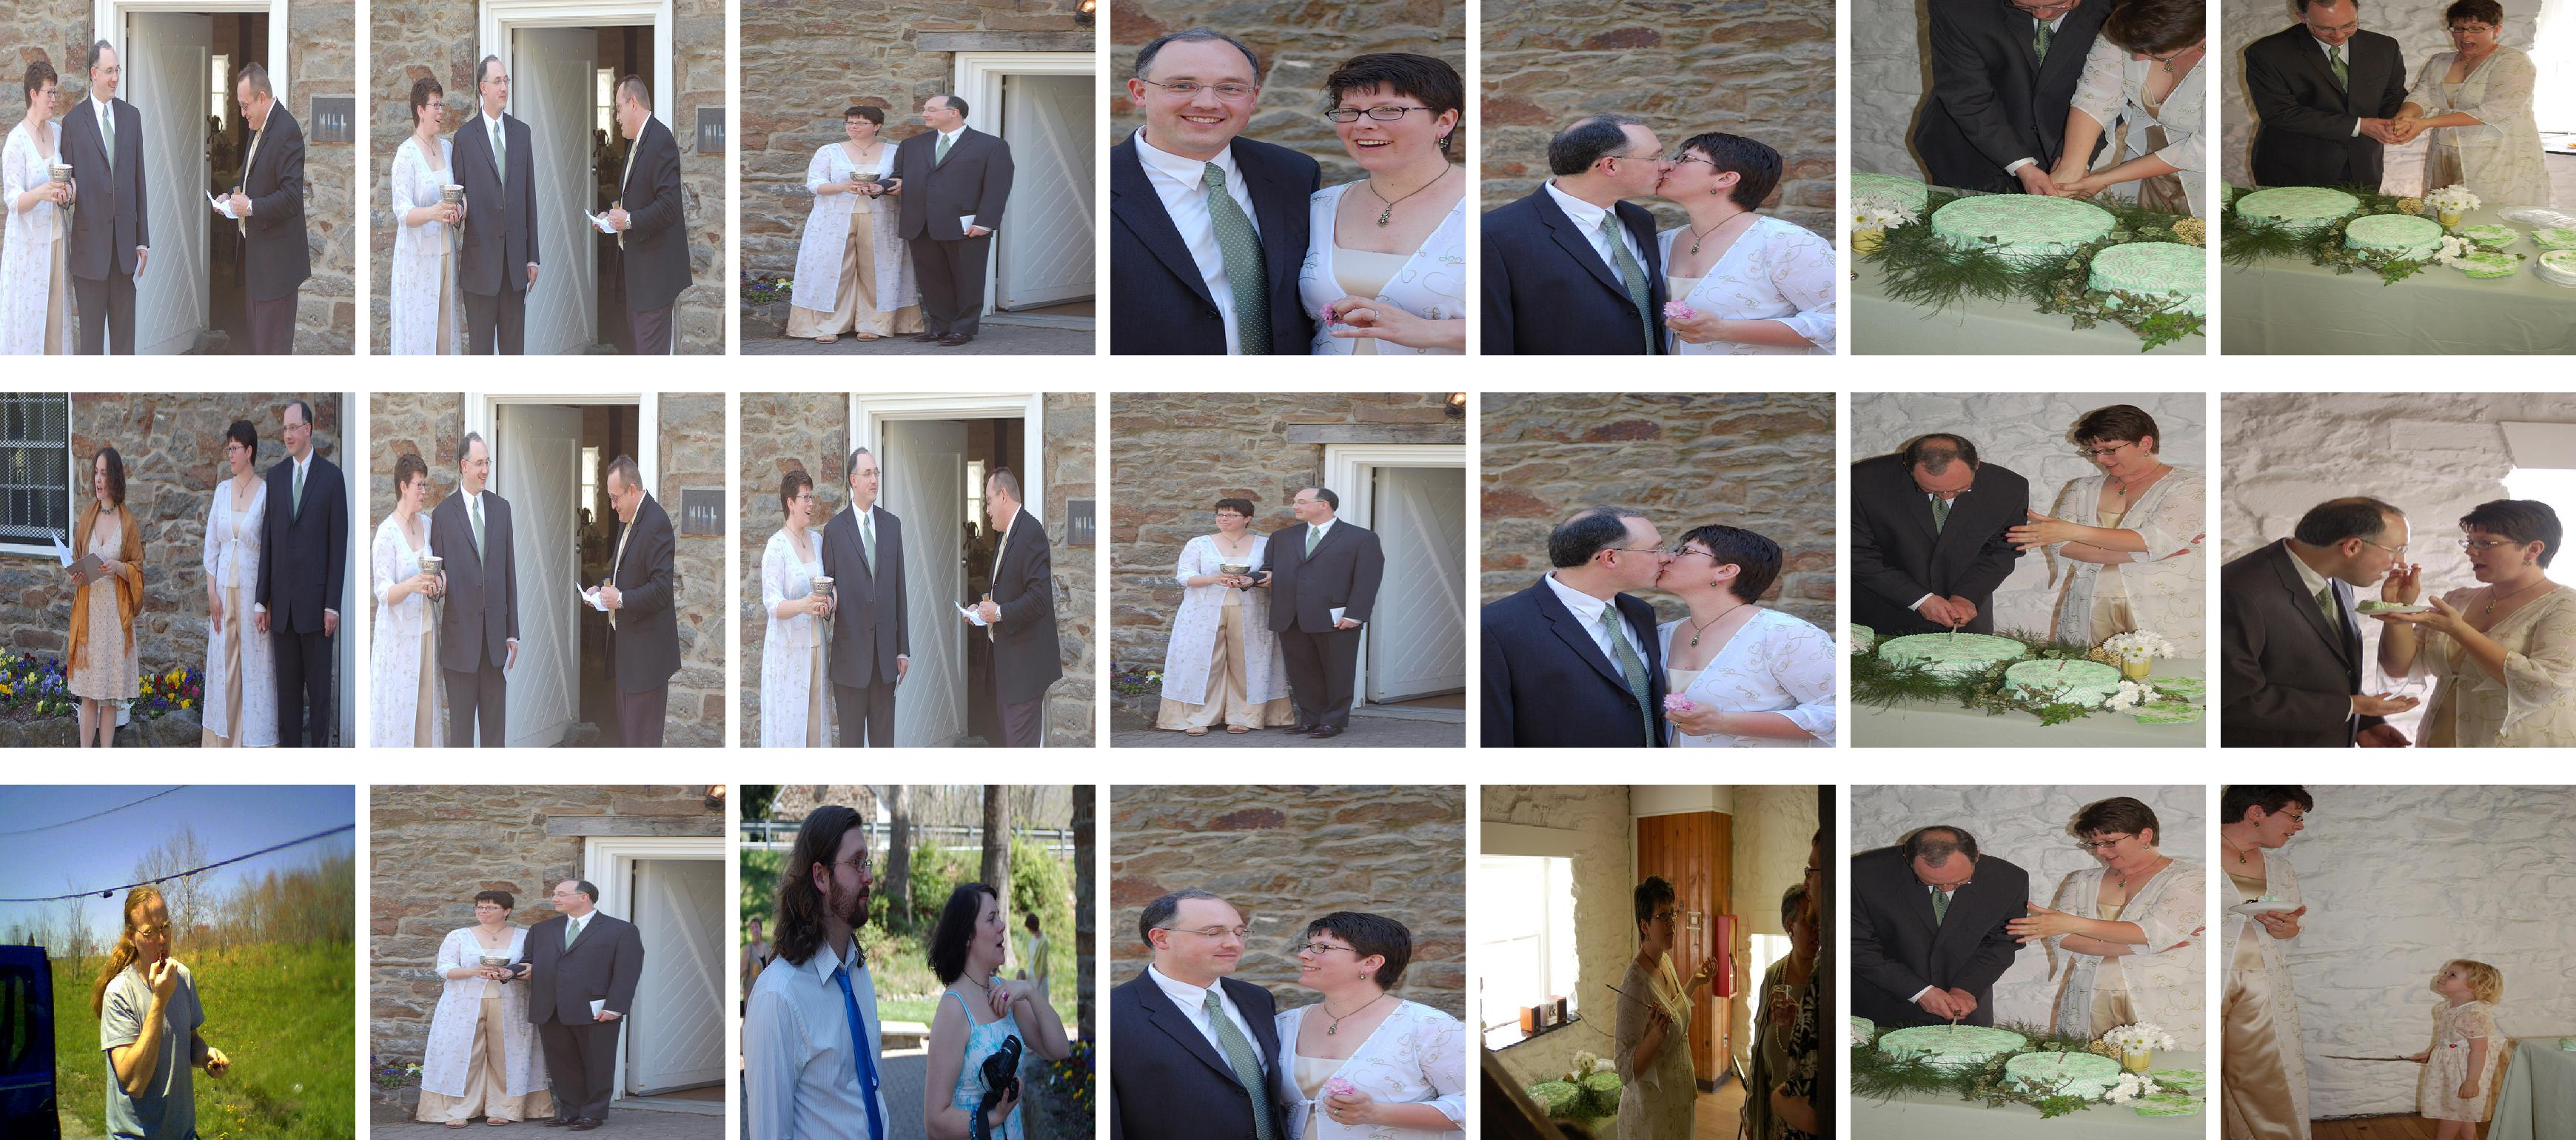
\includegraphics[height=1.5in]{results/a15_1_60509459@N00_7_20.jpg}} \hspace{2em}
  \subcaptionbox{Top 20\% of a \textit{Religious Activity} album. \label{fig26}}{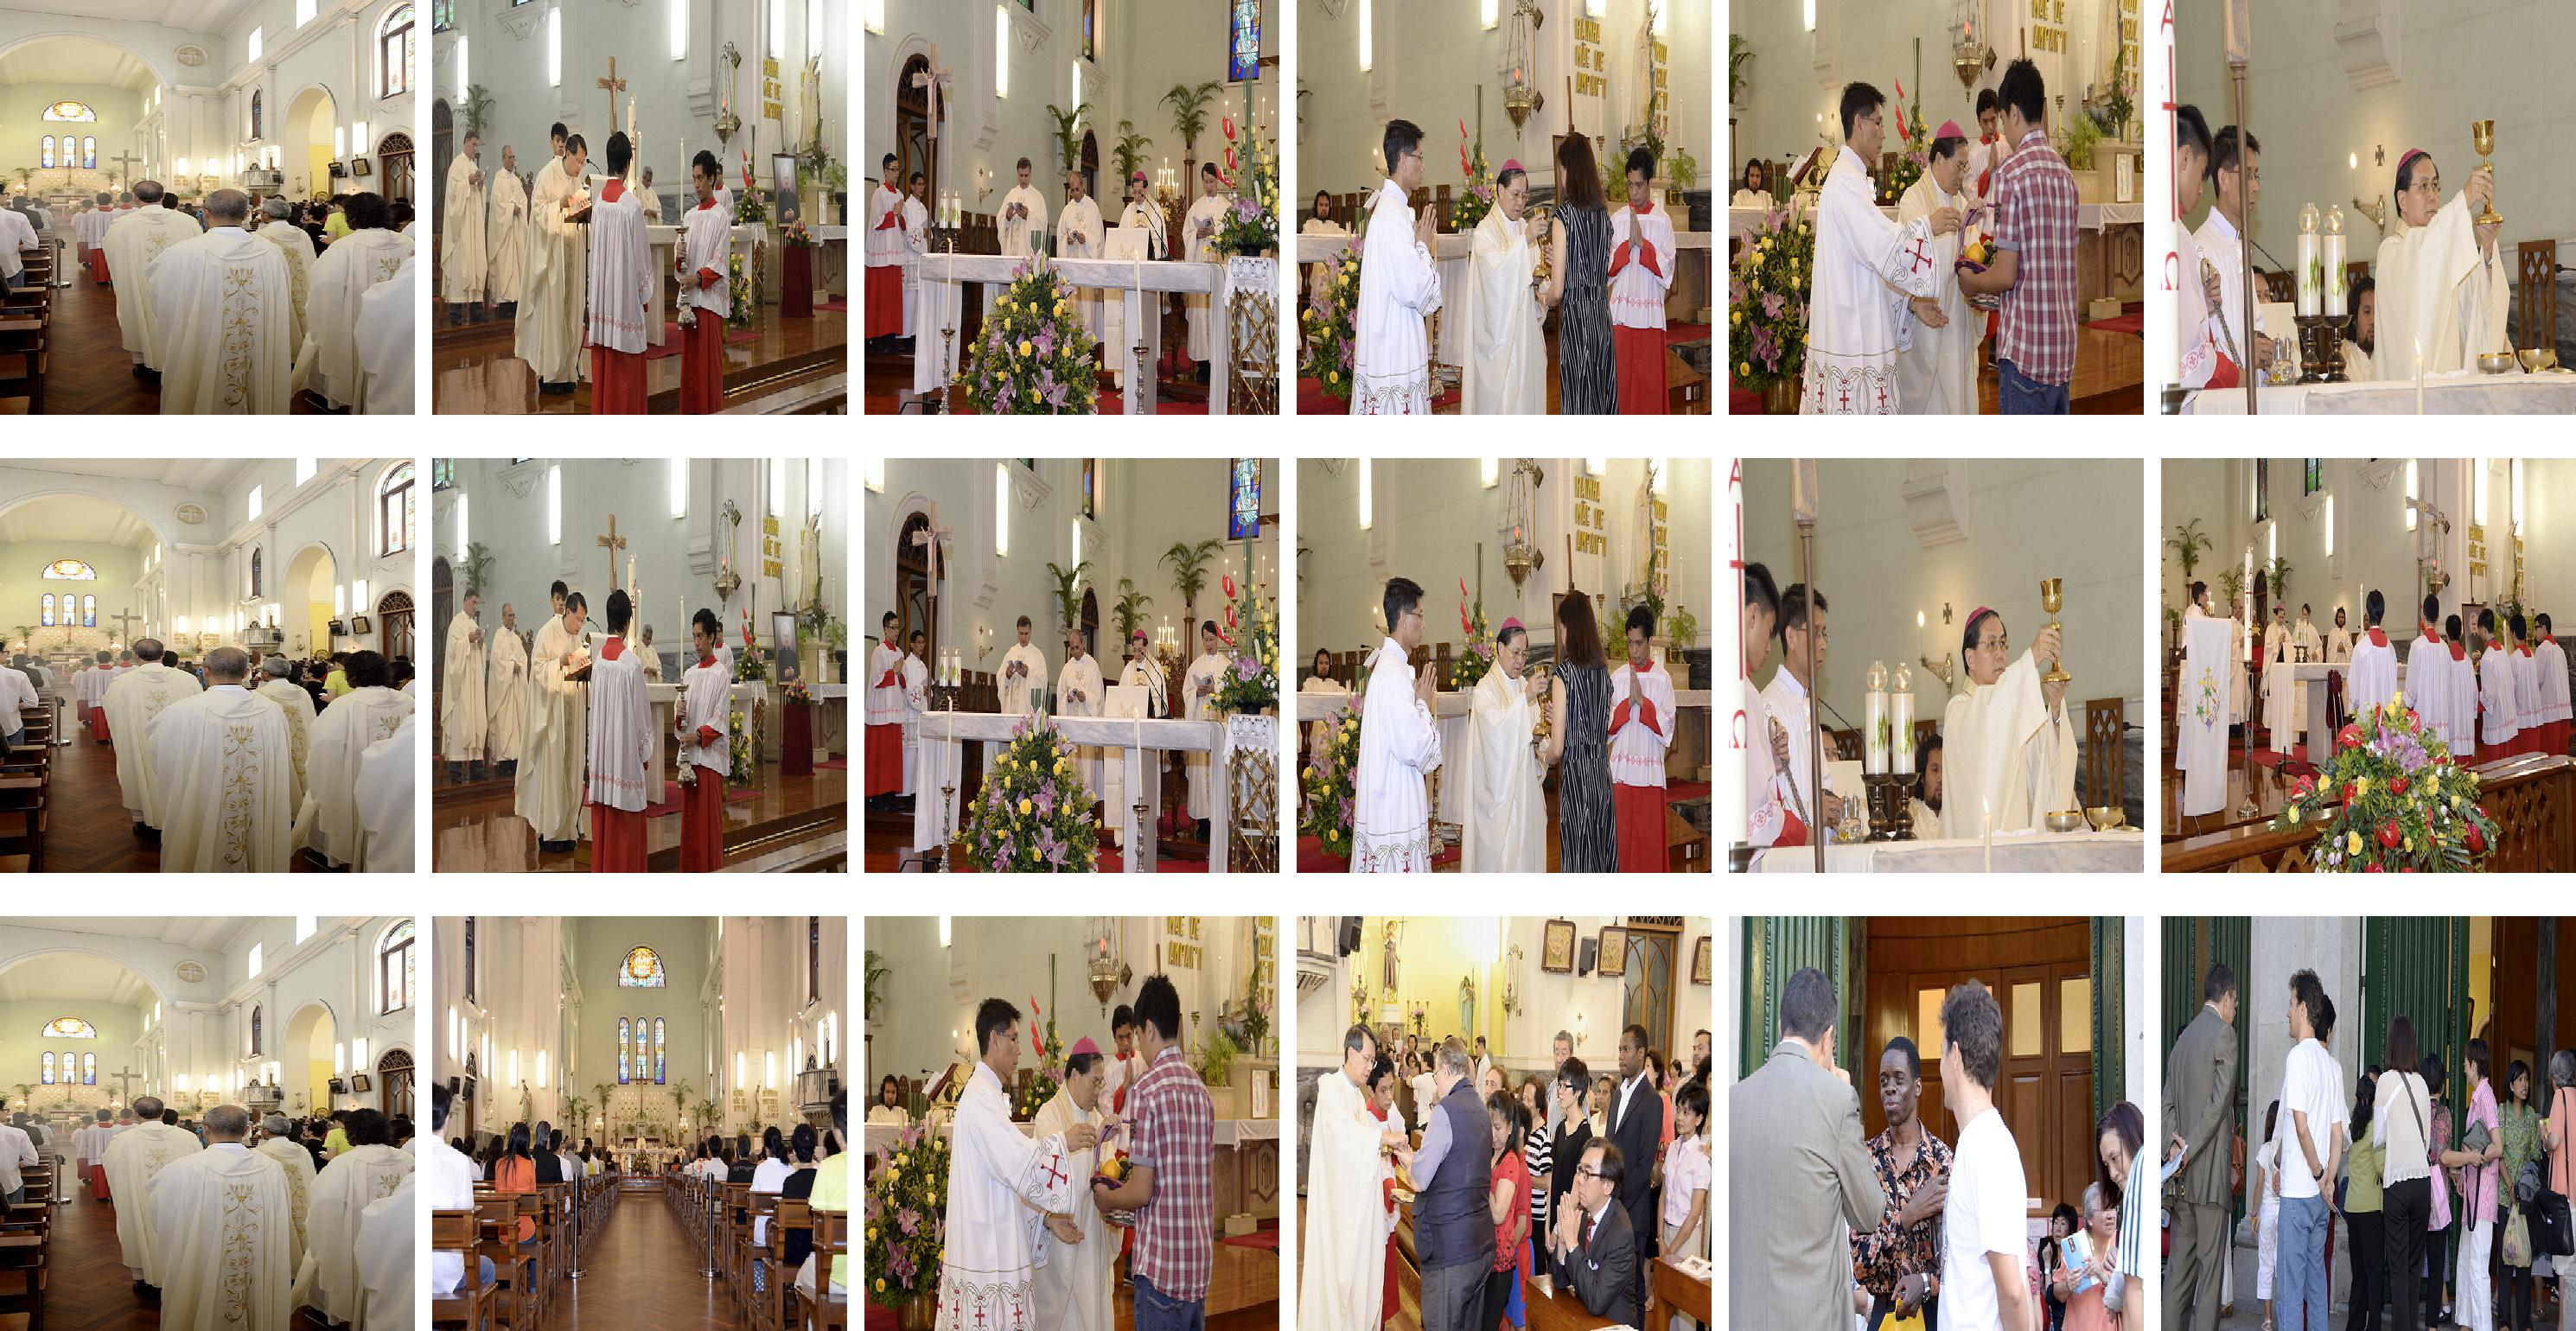
\includegraphics[height=1.5in]{results/a16_1_65675500@N00_6_20.jpg}}
  \subcaptionbox{Top 15\% of a \textit{Casual Family/Friends Gathering} album. \label{fig27}}{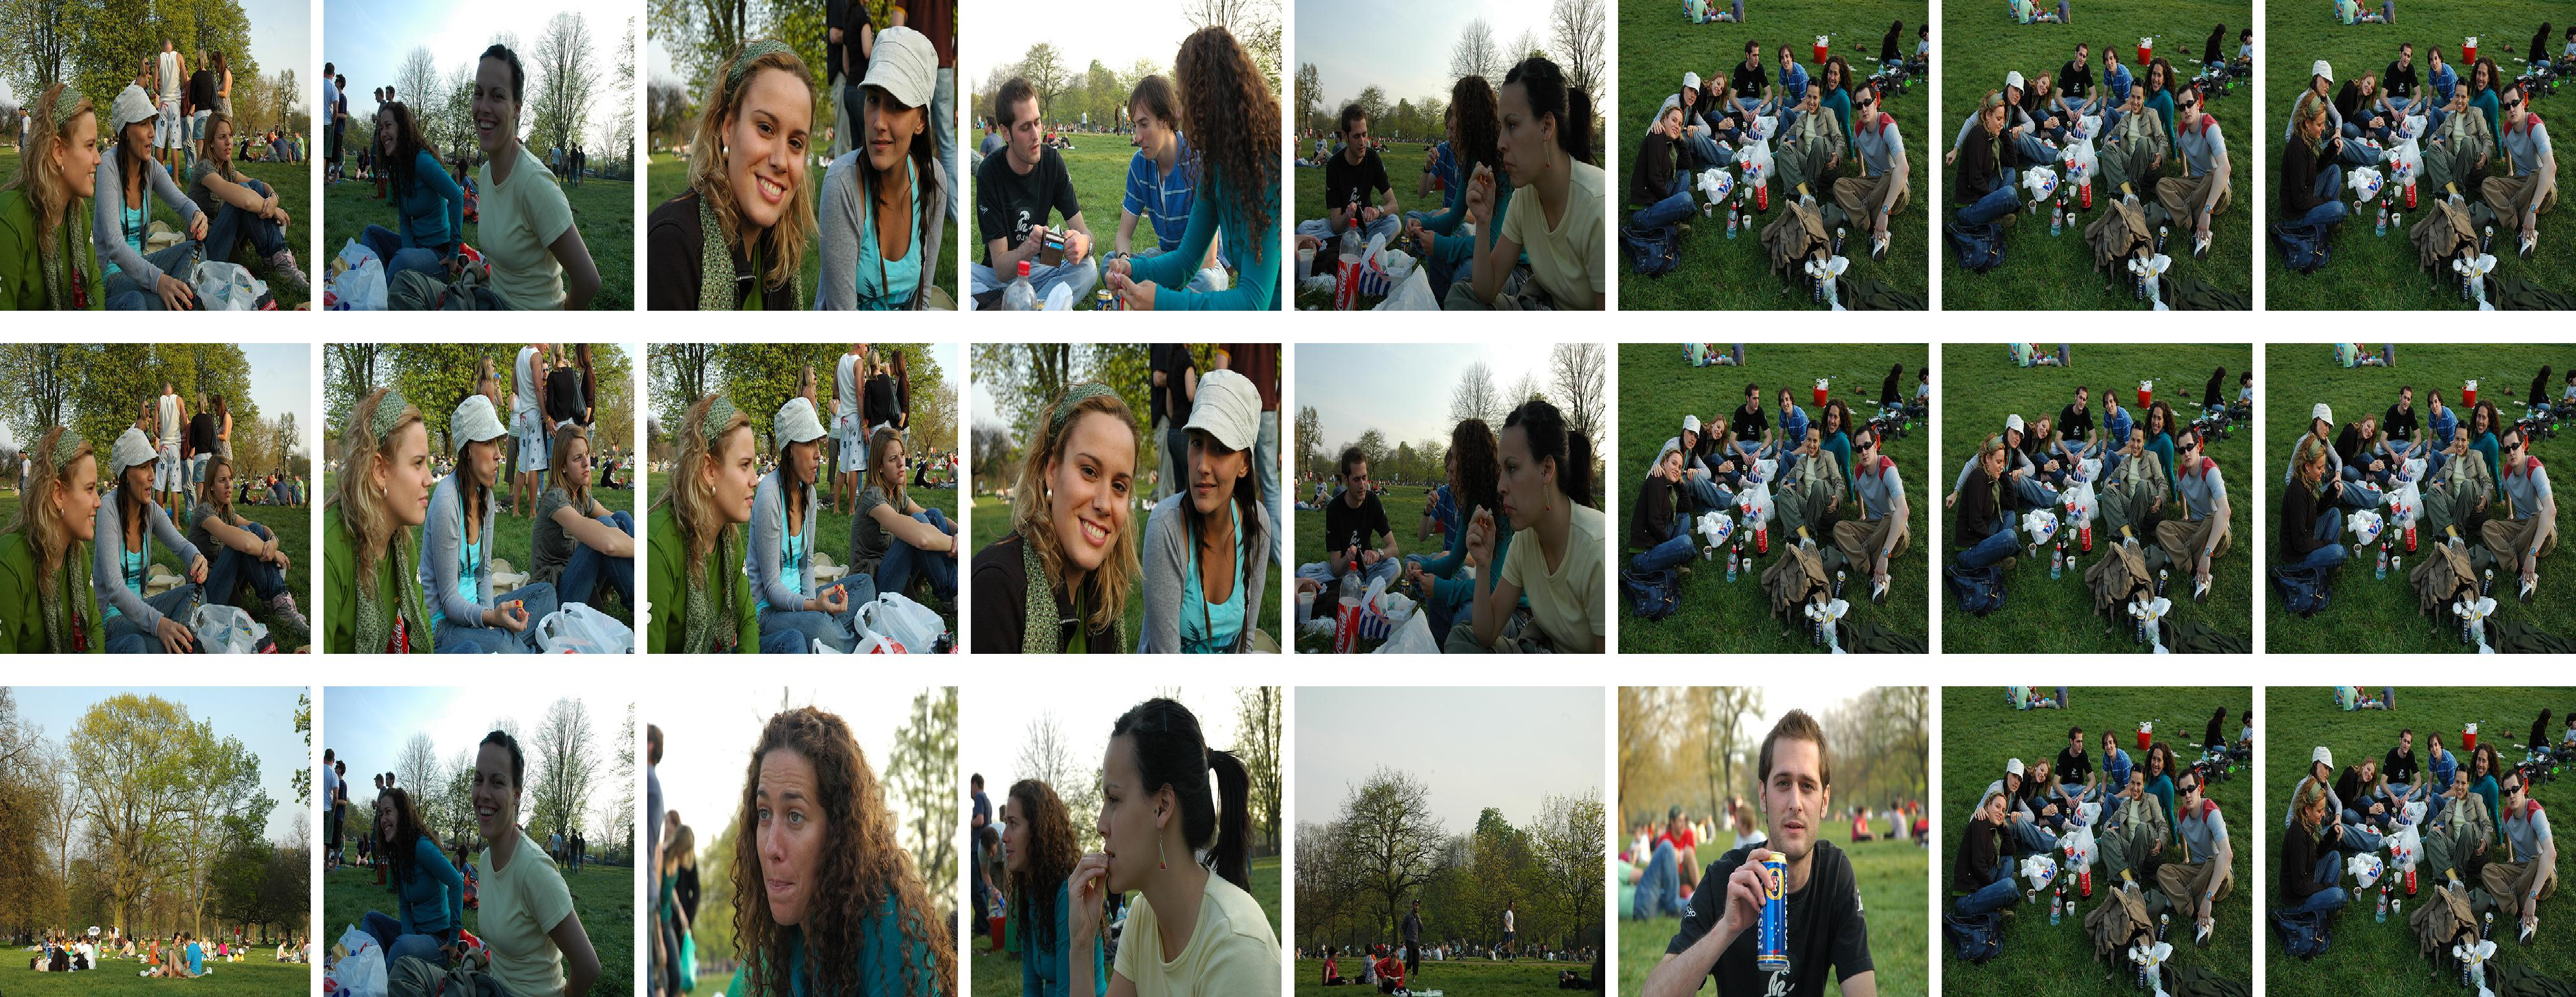
\includegraphics[height=1.5in]{results/a17_1_66263830@N00_8_15.jpg}}
  \subcaptionbox{Top 20\% of a \textit{Wedding} album. \label{fig28}}{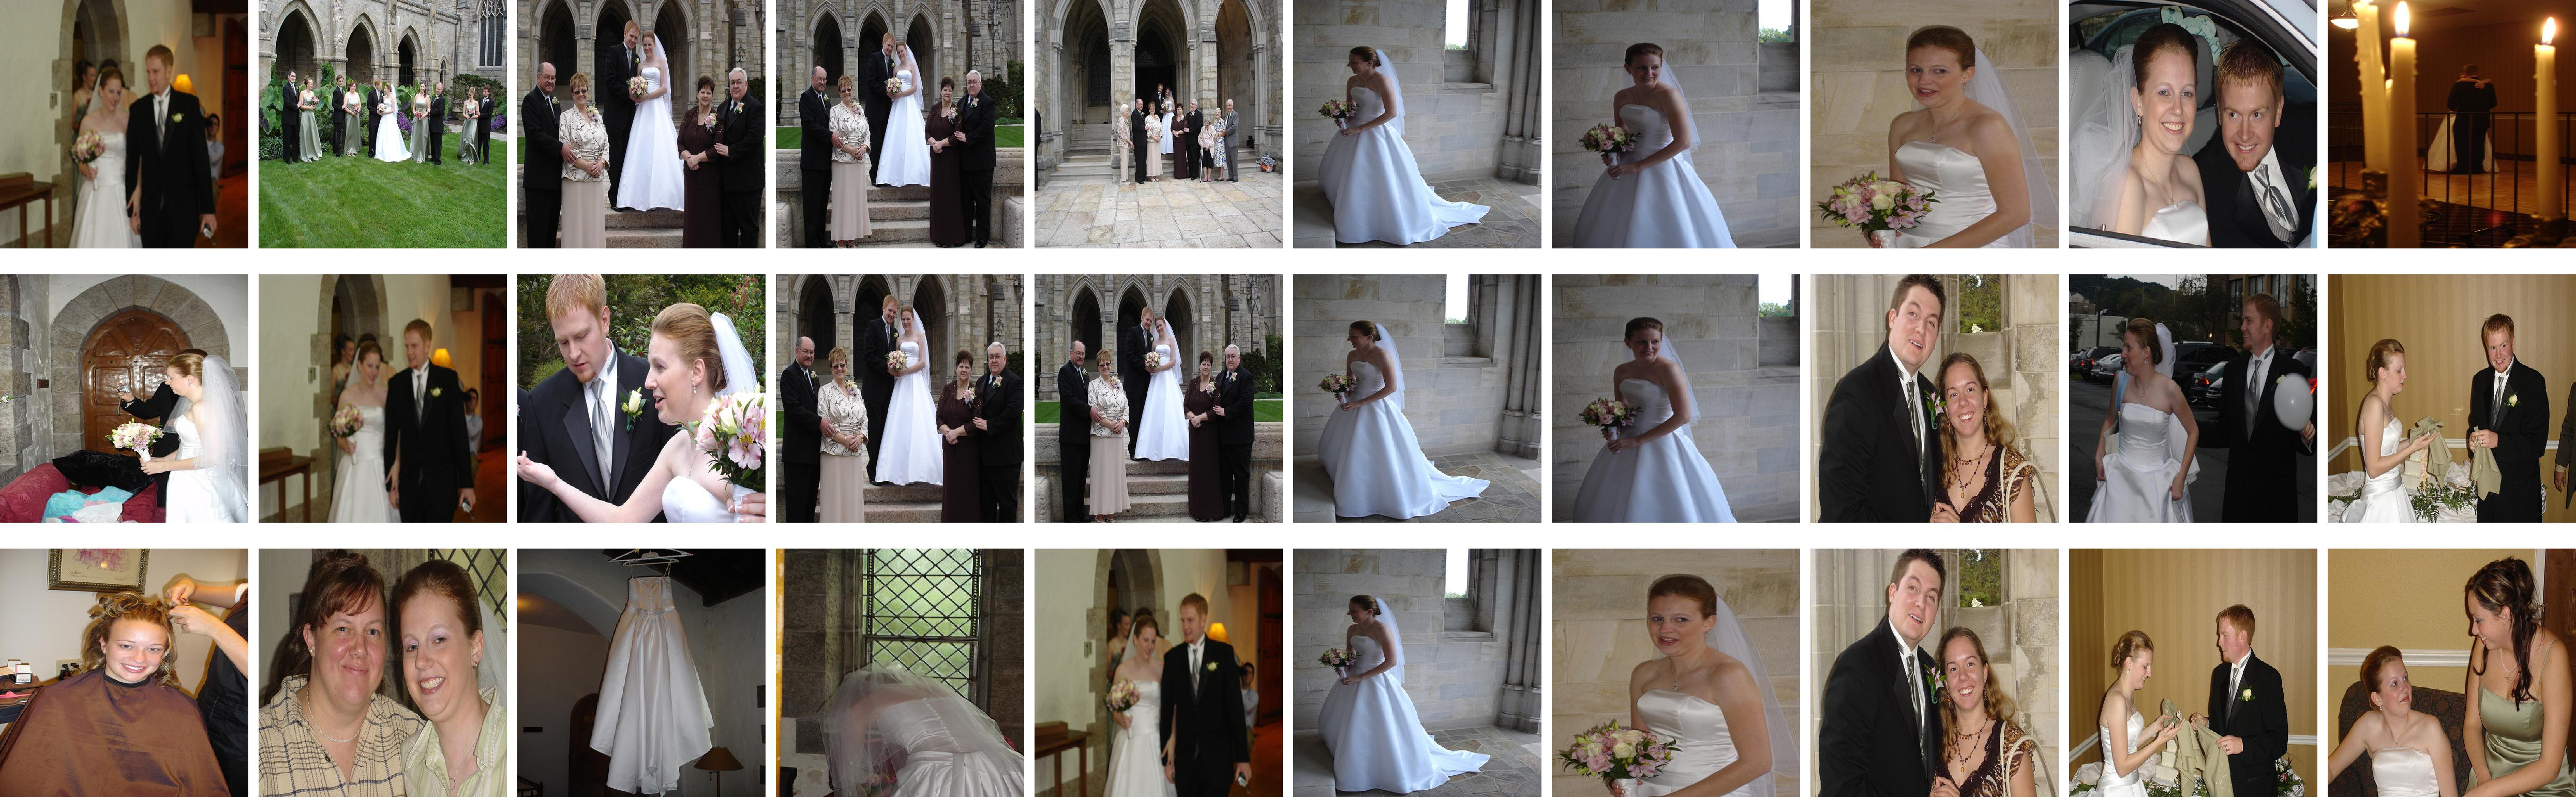
\includegraphics[height=1.5in]{results/a18_1_82802179@N00_10_20.jpg}}
      \end{figure*}
  
\clearpage
  \begin{figure*}[ht]
  \ContinuedFloat % continue from previous page
\centering
  \subcaptionbox{Top 20\% of a \textit{Birthday} album. \label{fig29}}{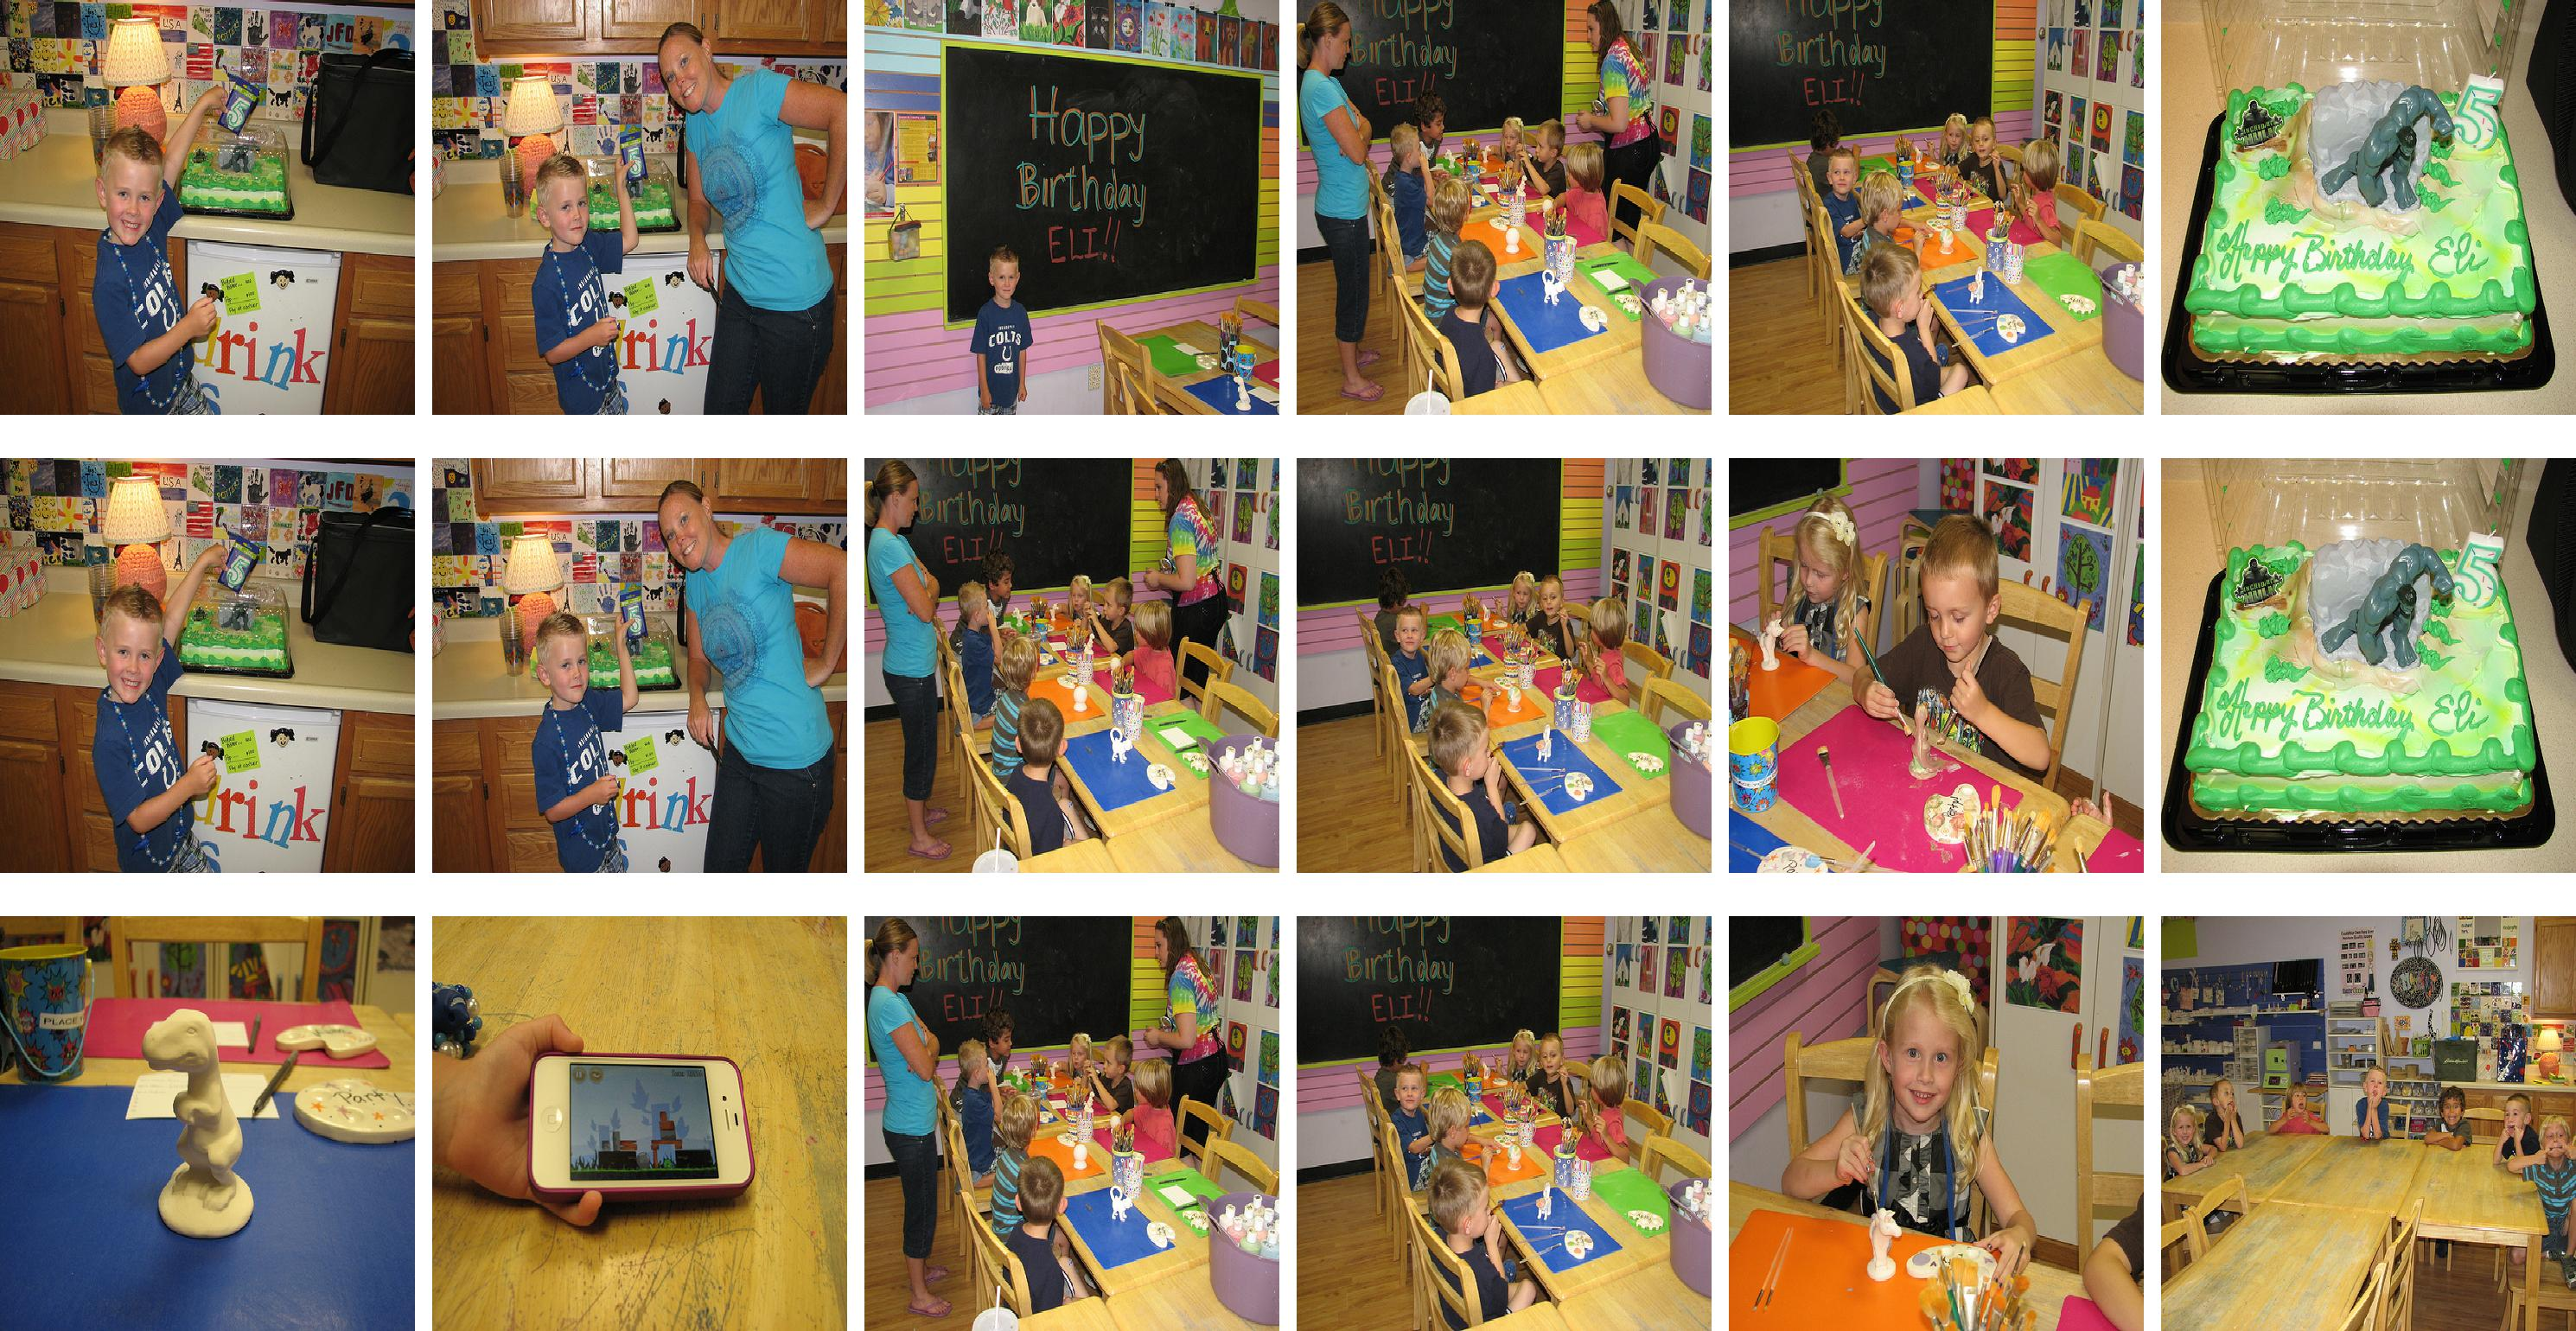
\includegraphics[height=1.5in]{results/a19_17_44124461706@N01_6_20.jpg}} \hspace{2em}
%  \subcaptionbox{Top 20\% of a \textit{Halloween} album. \label{fig30}}{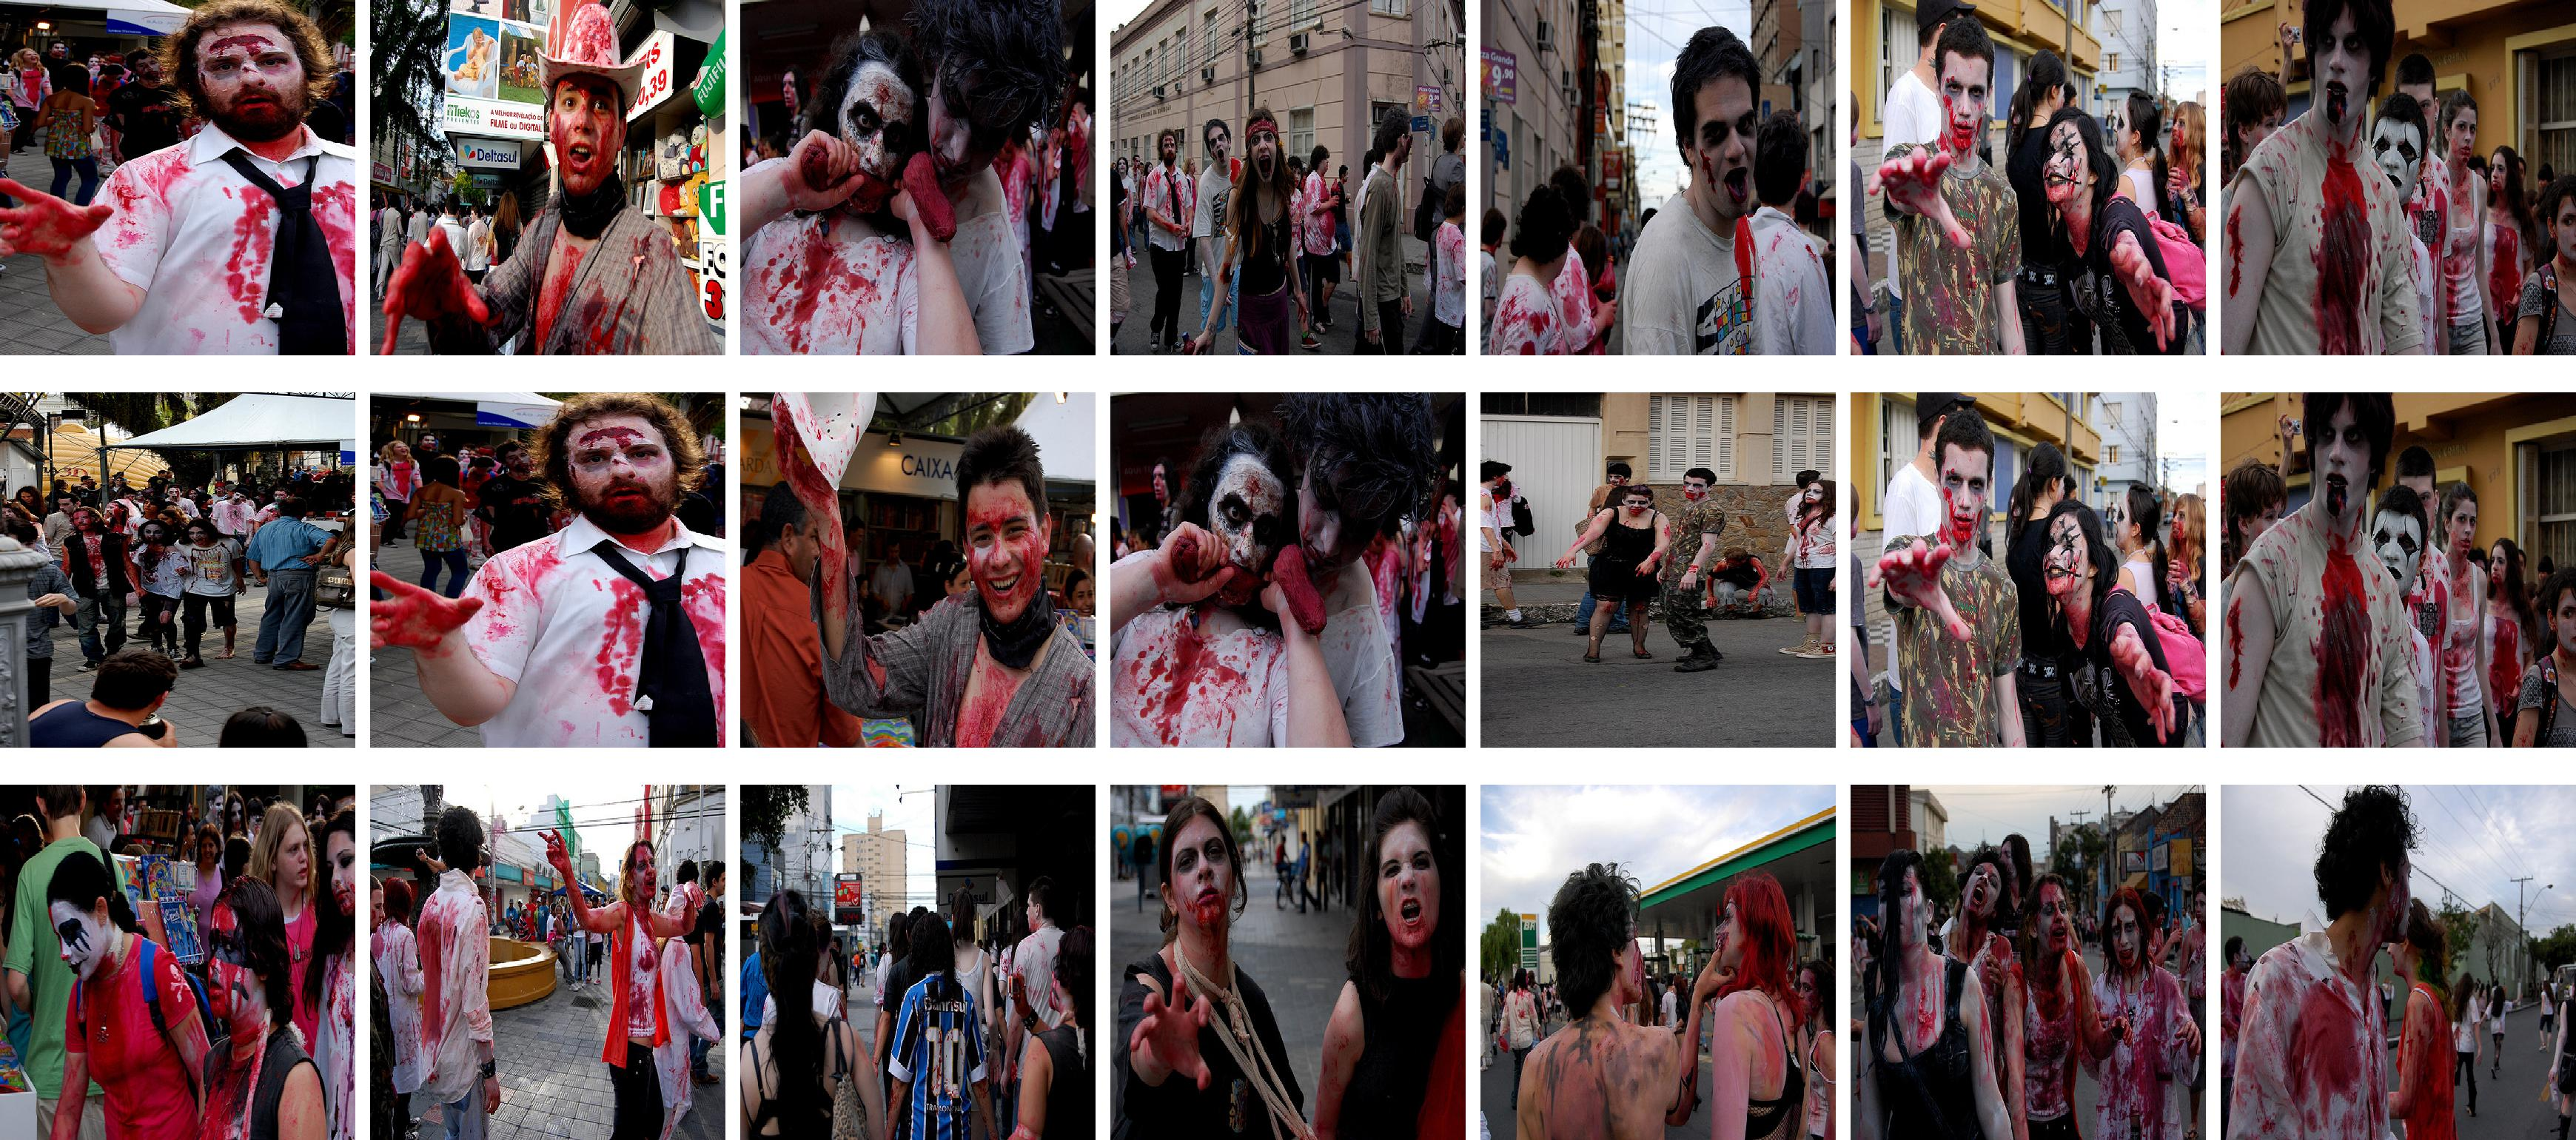
\includegraphics[height=1.5in]{results/a20_1_30764740@N07_7_20.jpg}}
  \subcaptionbox{Top 20\% of a \textit{Halloween} album. \label{fig30}}{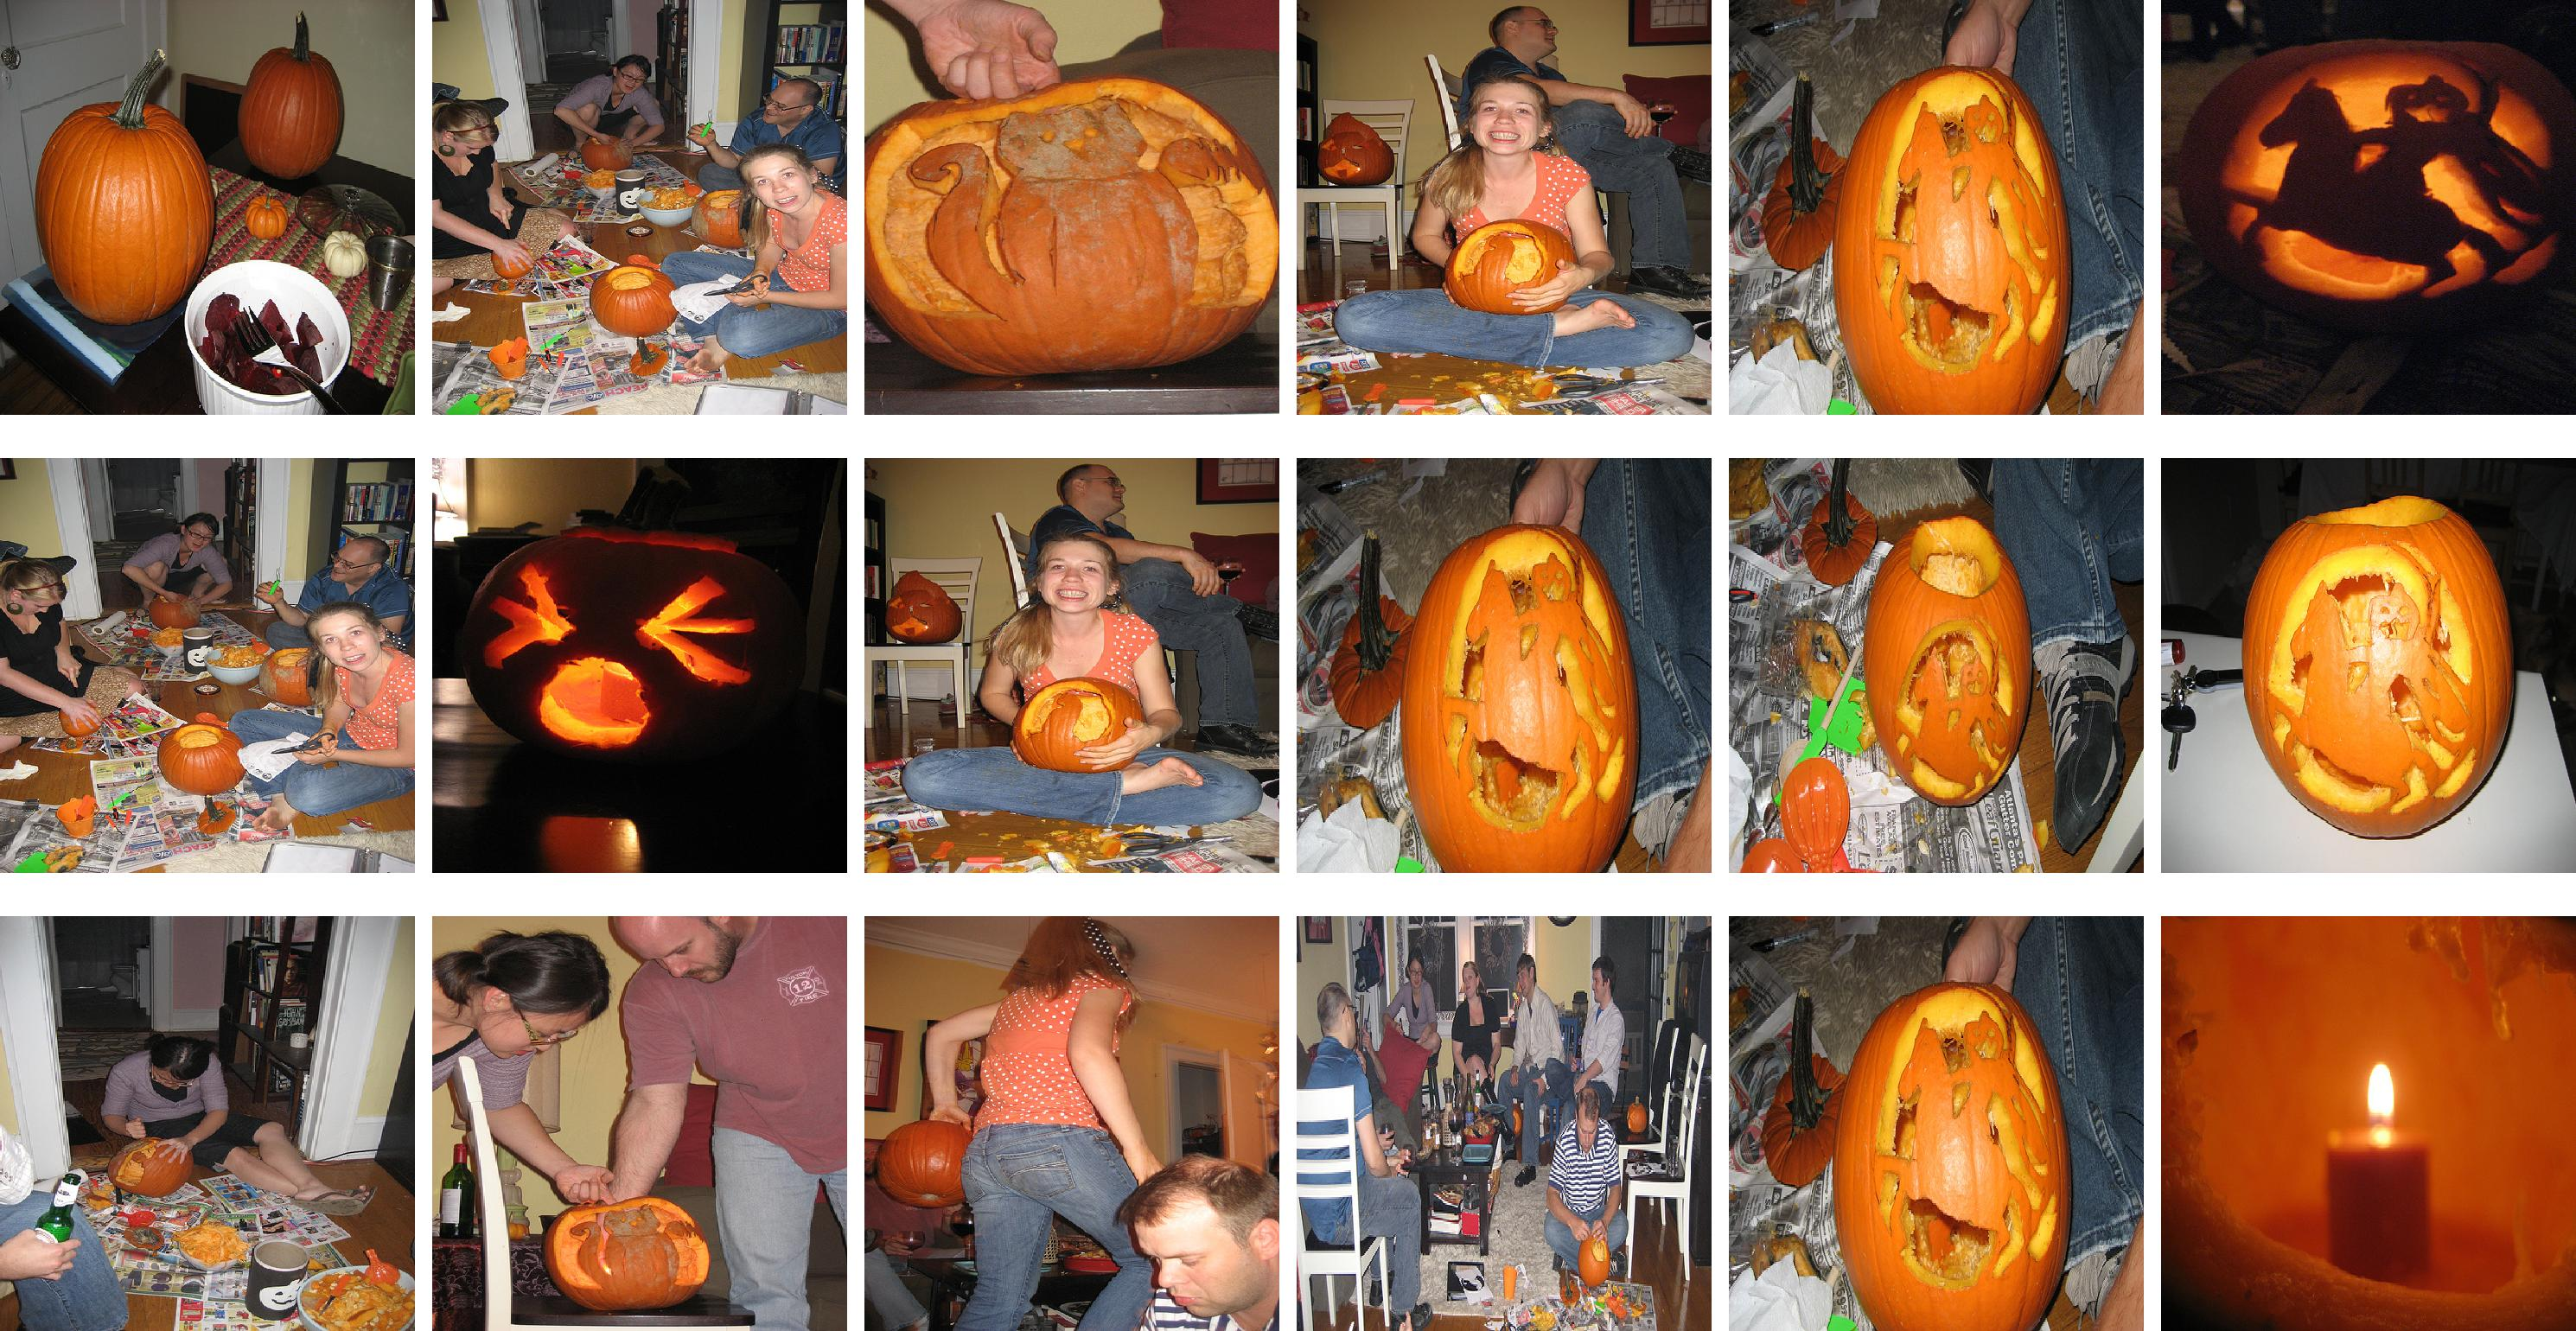
\includegraphics[height=1.5in]{results/Halloween/7_54788523@N00_6_20.jpg}}
  \subcaptionbox{Top 20\% of a \textit{Birthday} album. \label{fig31}}{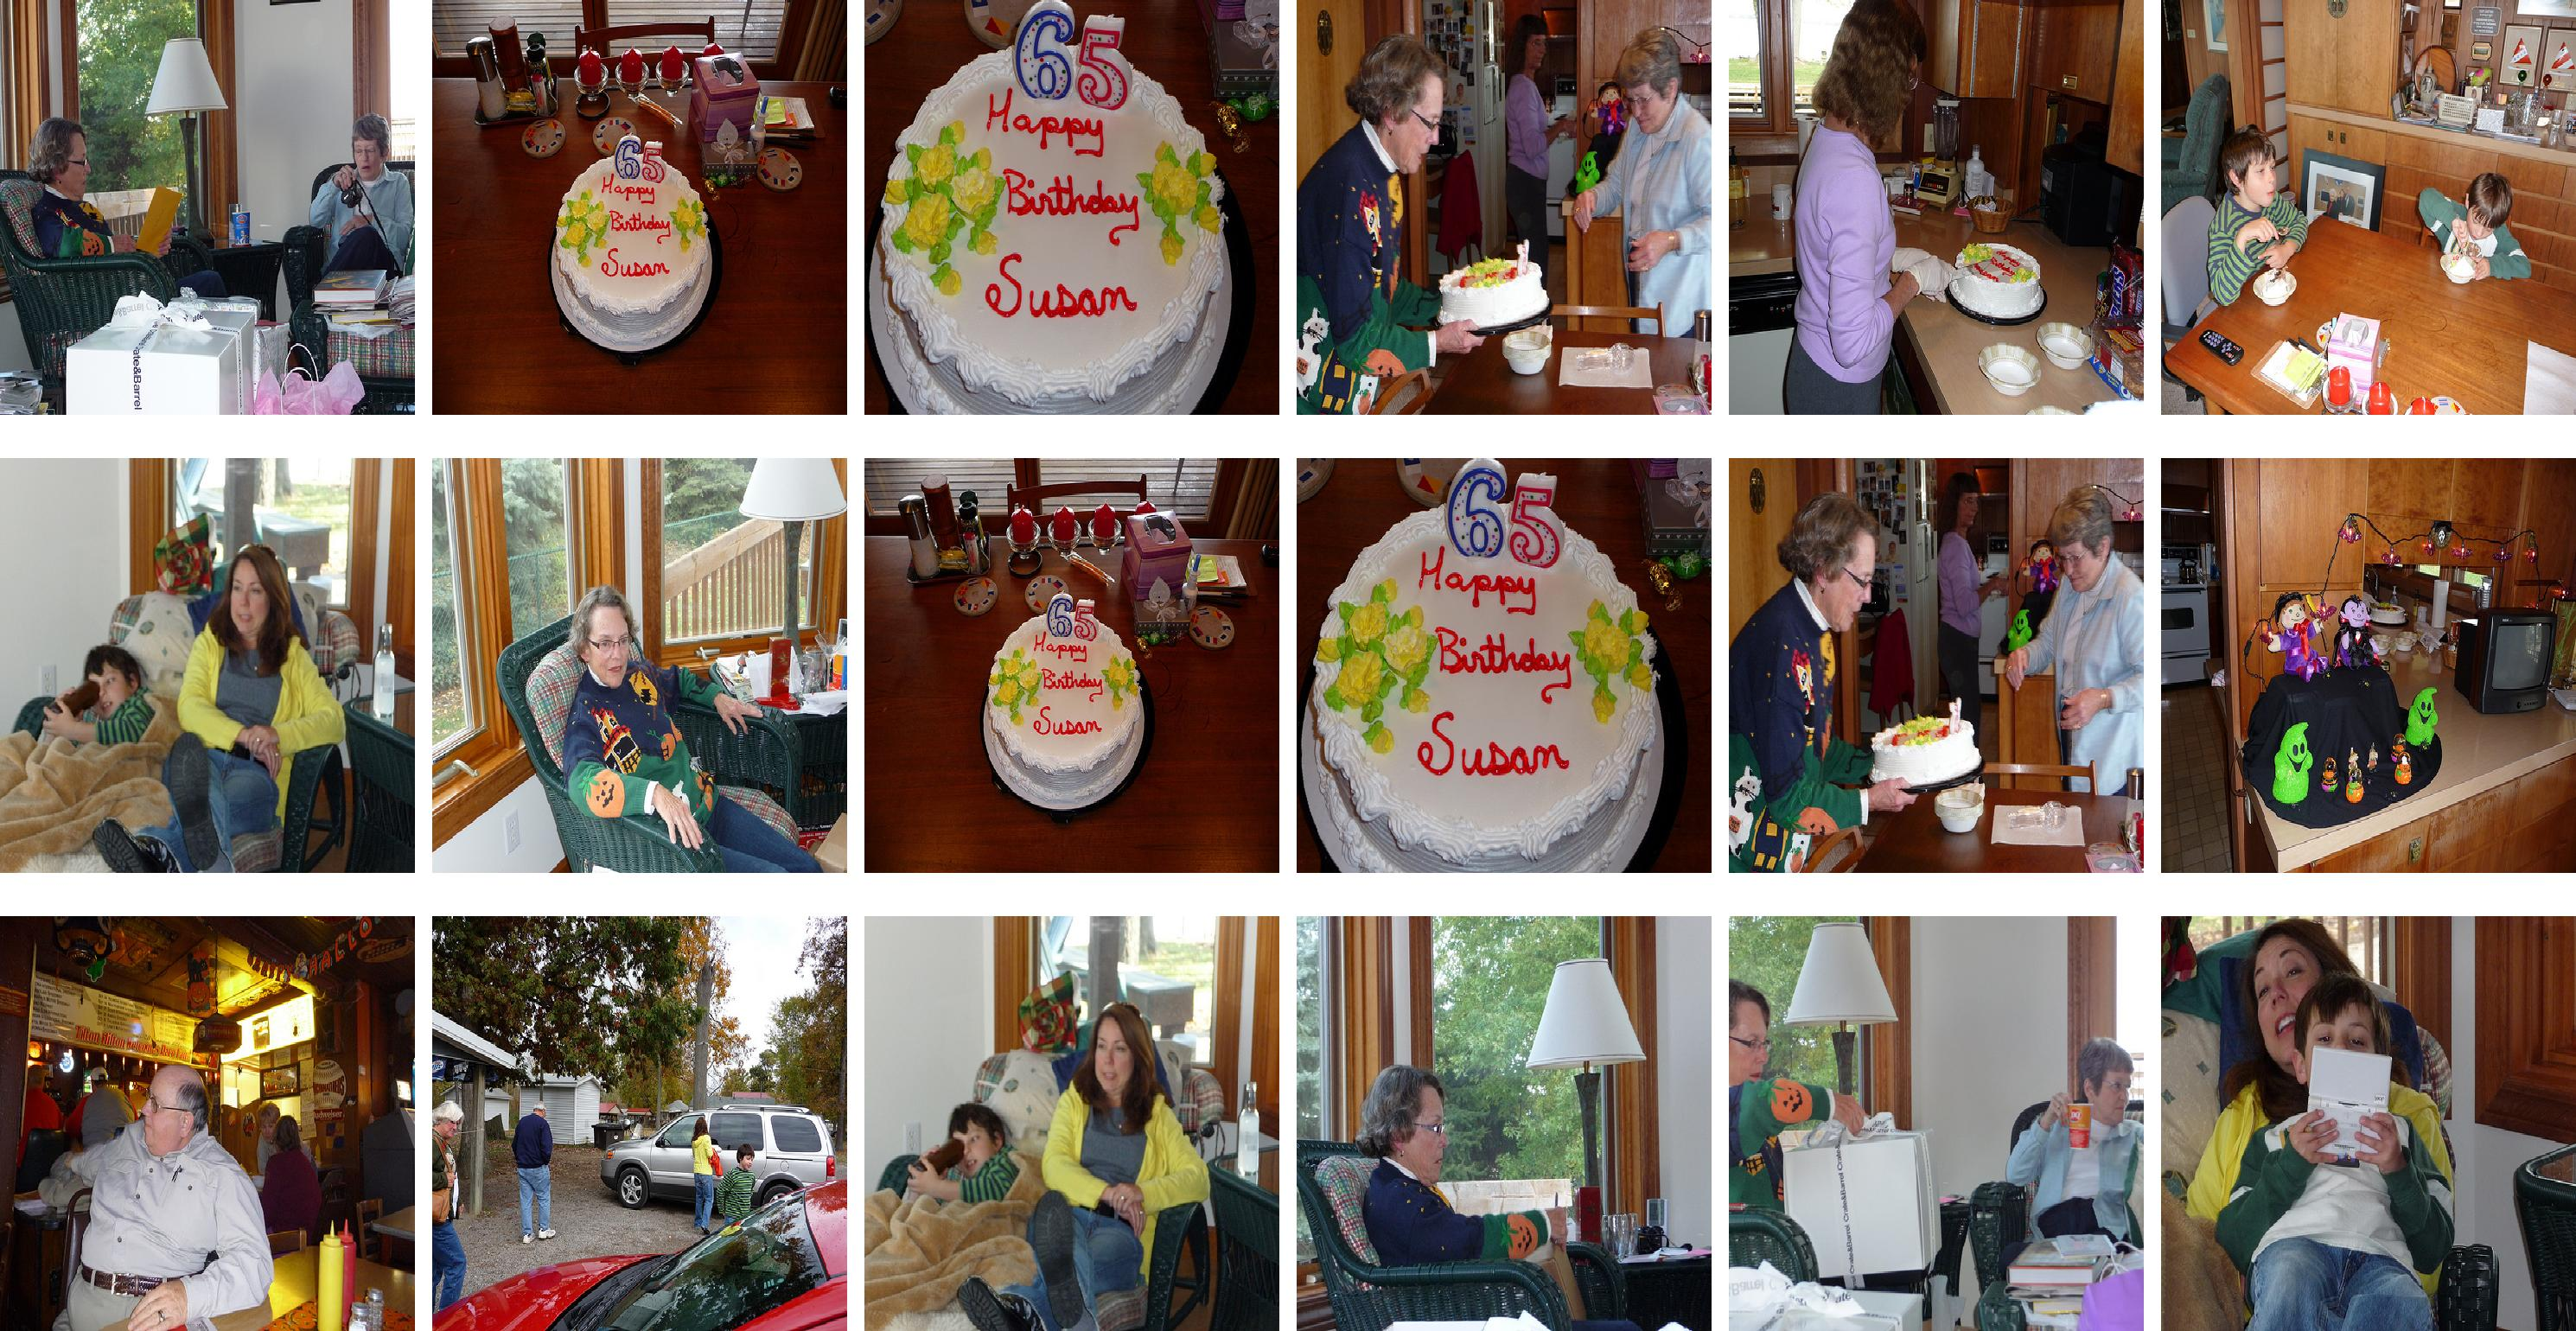
\includegraphics[height=1.5in]{results/a21_1_28004076@N04_6_20.jpg}} \hspace{2em}
  \subcaptionbox{Top 20\% of a \textit{Wedding} album. \label{fig32}}{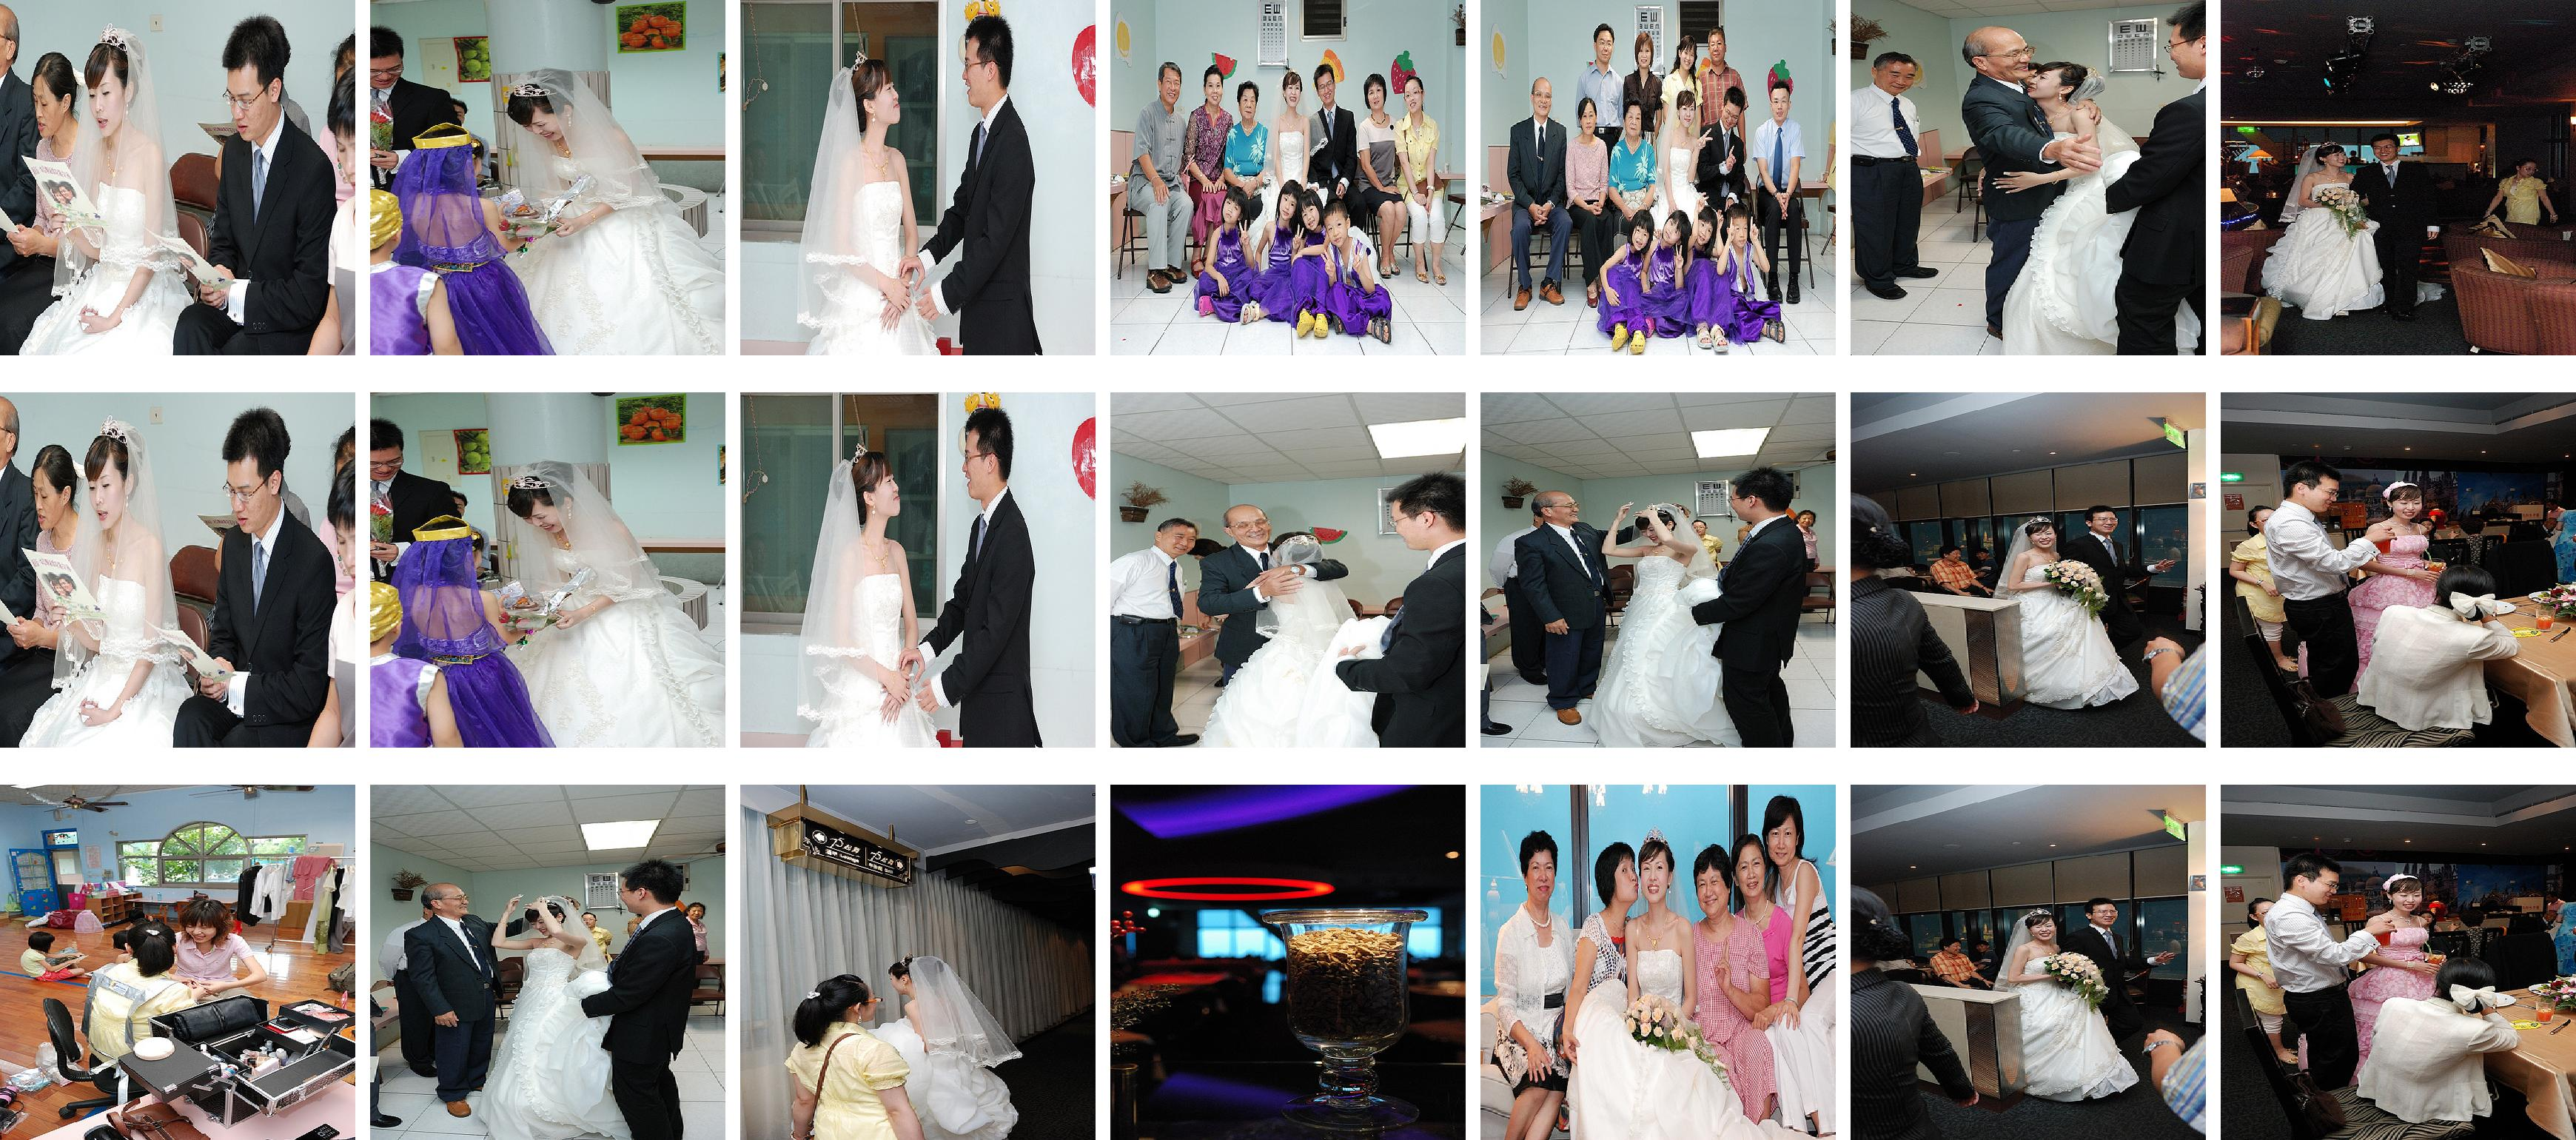
\includegraphics[height=1.5in]{results/a22_1_7614607@N05_7_20.jpg}}
  \subcaptionbox{Top 20\% of a \textit{Zoo} album. \label{fig33}}{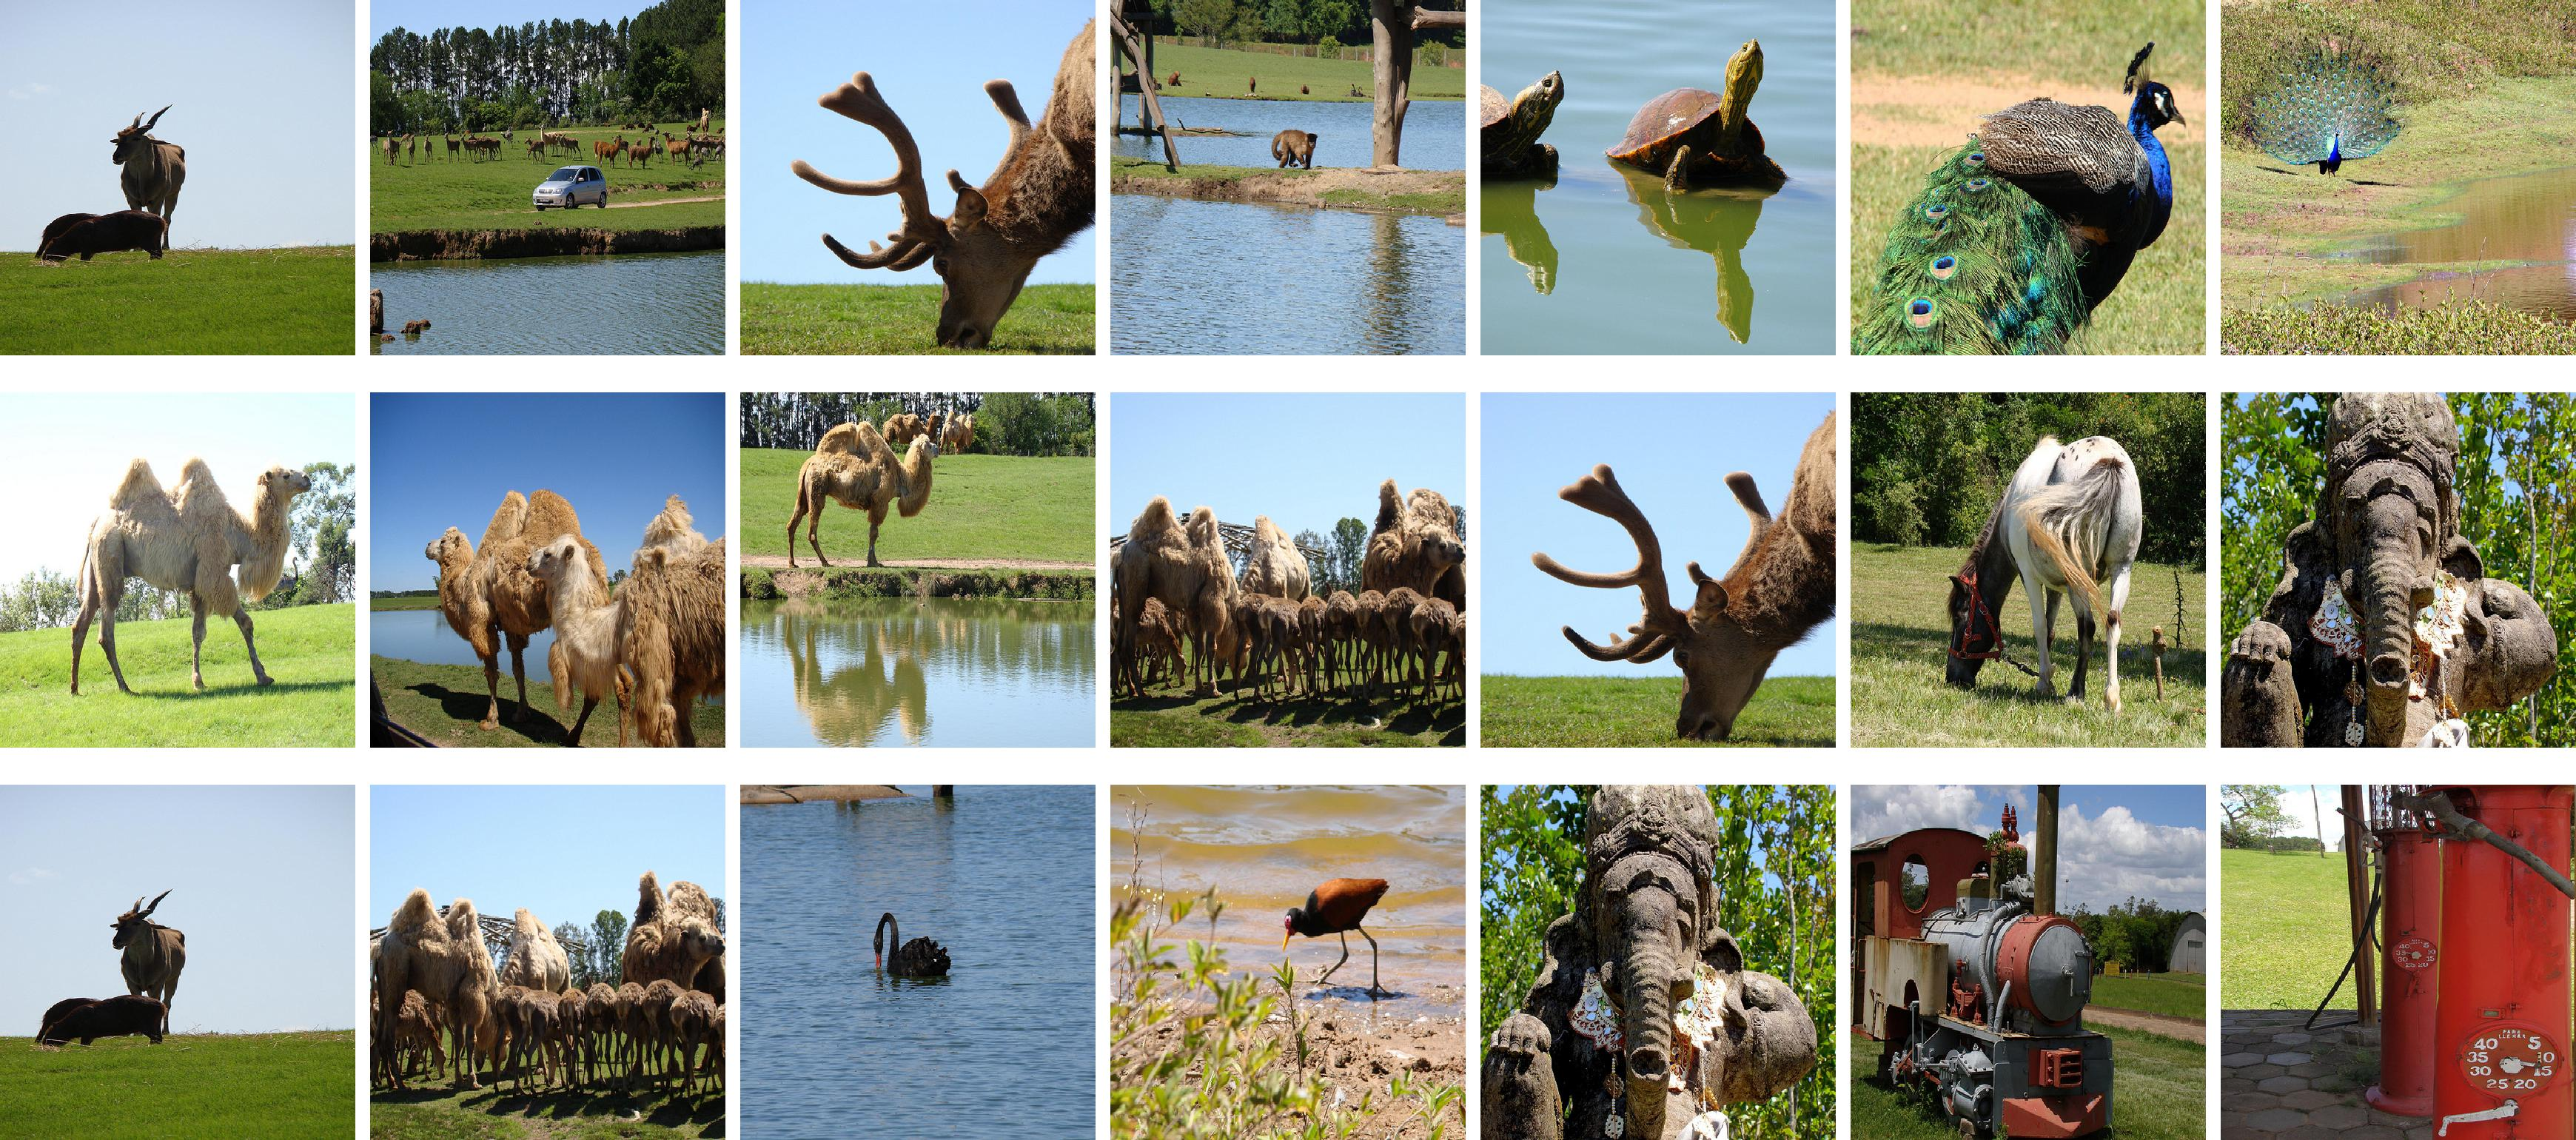
\includegraphics[height=1.5in]{results/a23_1_42943151@N06_7_20.jpg}} \hspace{2em}
    \subcaptionbox{Top 20\% of a \textit{Halloween} album. \label{fig34}}{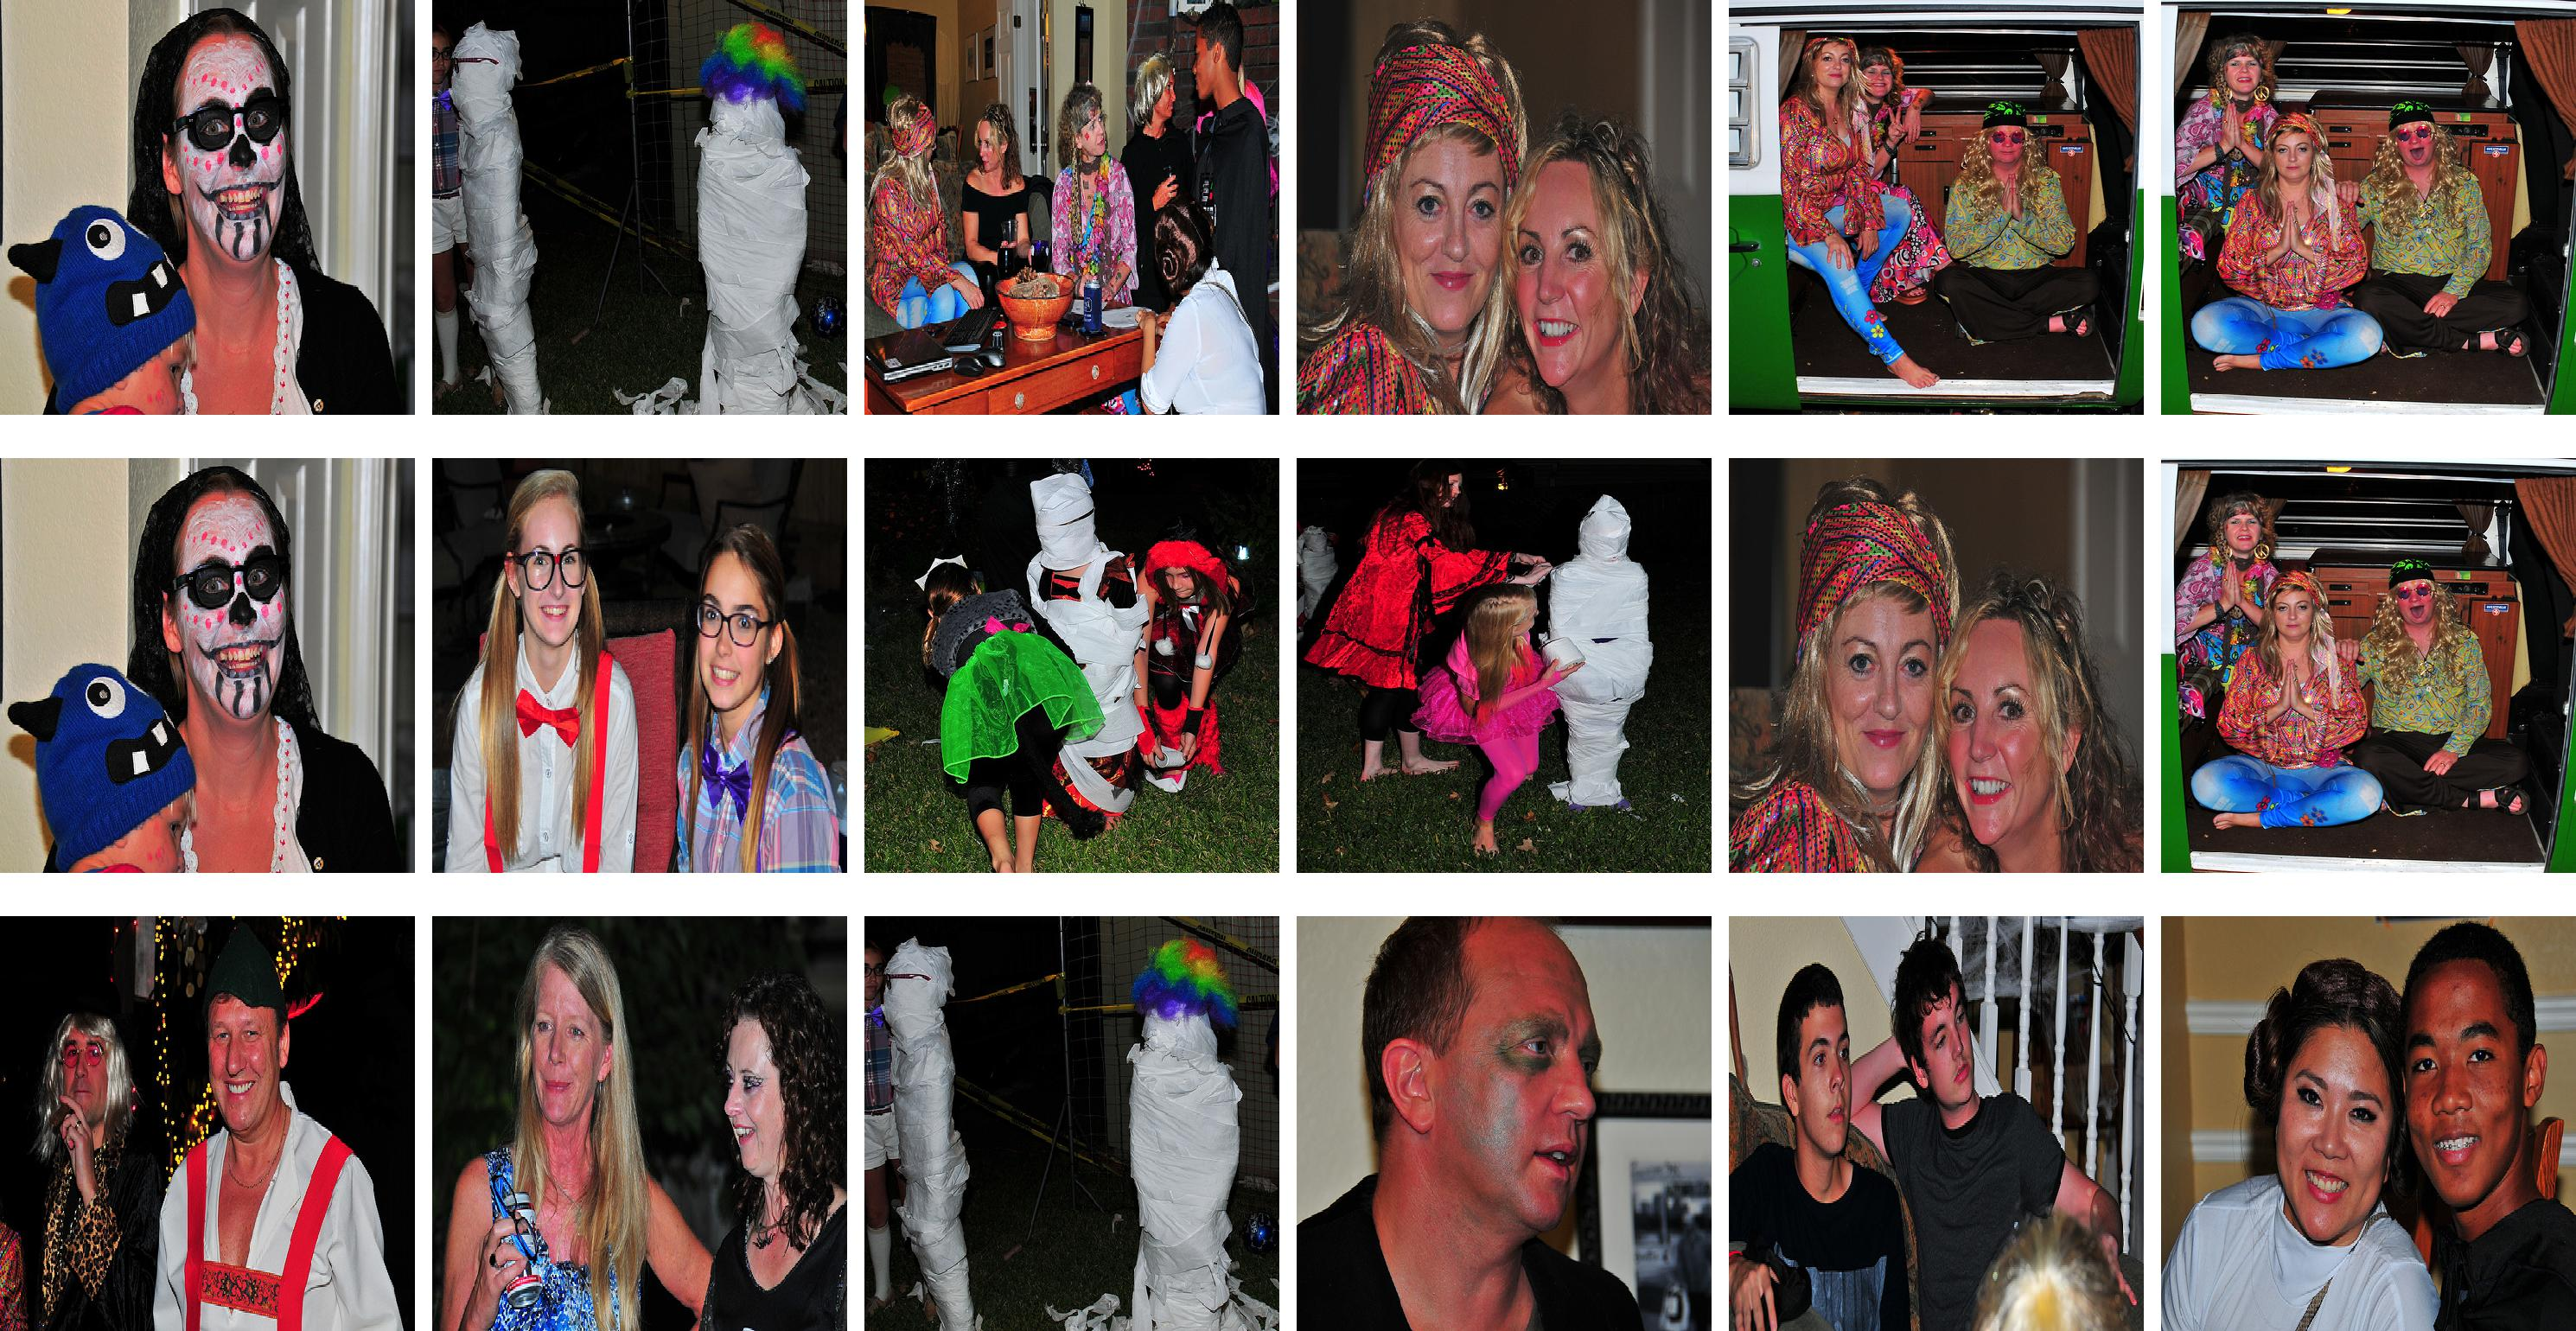
\includegraphics[height=1.5in]{results/Halloween/0_17746744@N08_6_20.jpg}}
%    \subcaptionbox{Top 20\% of a \textit{Halloween} album. \label{fig34}}{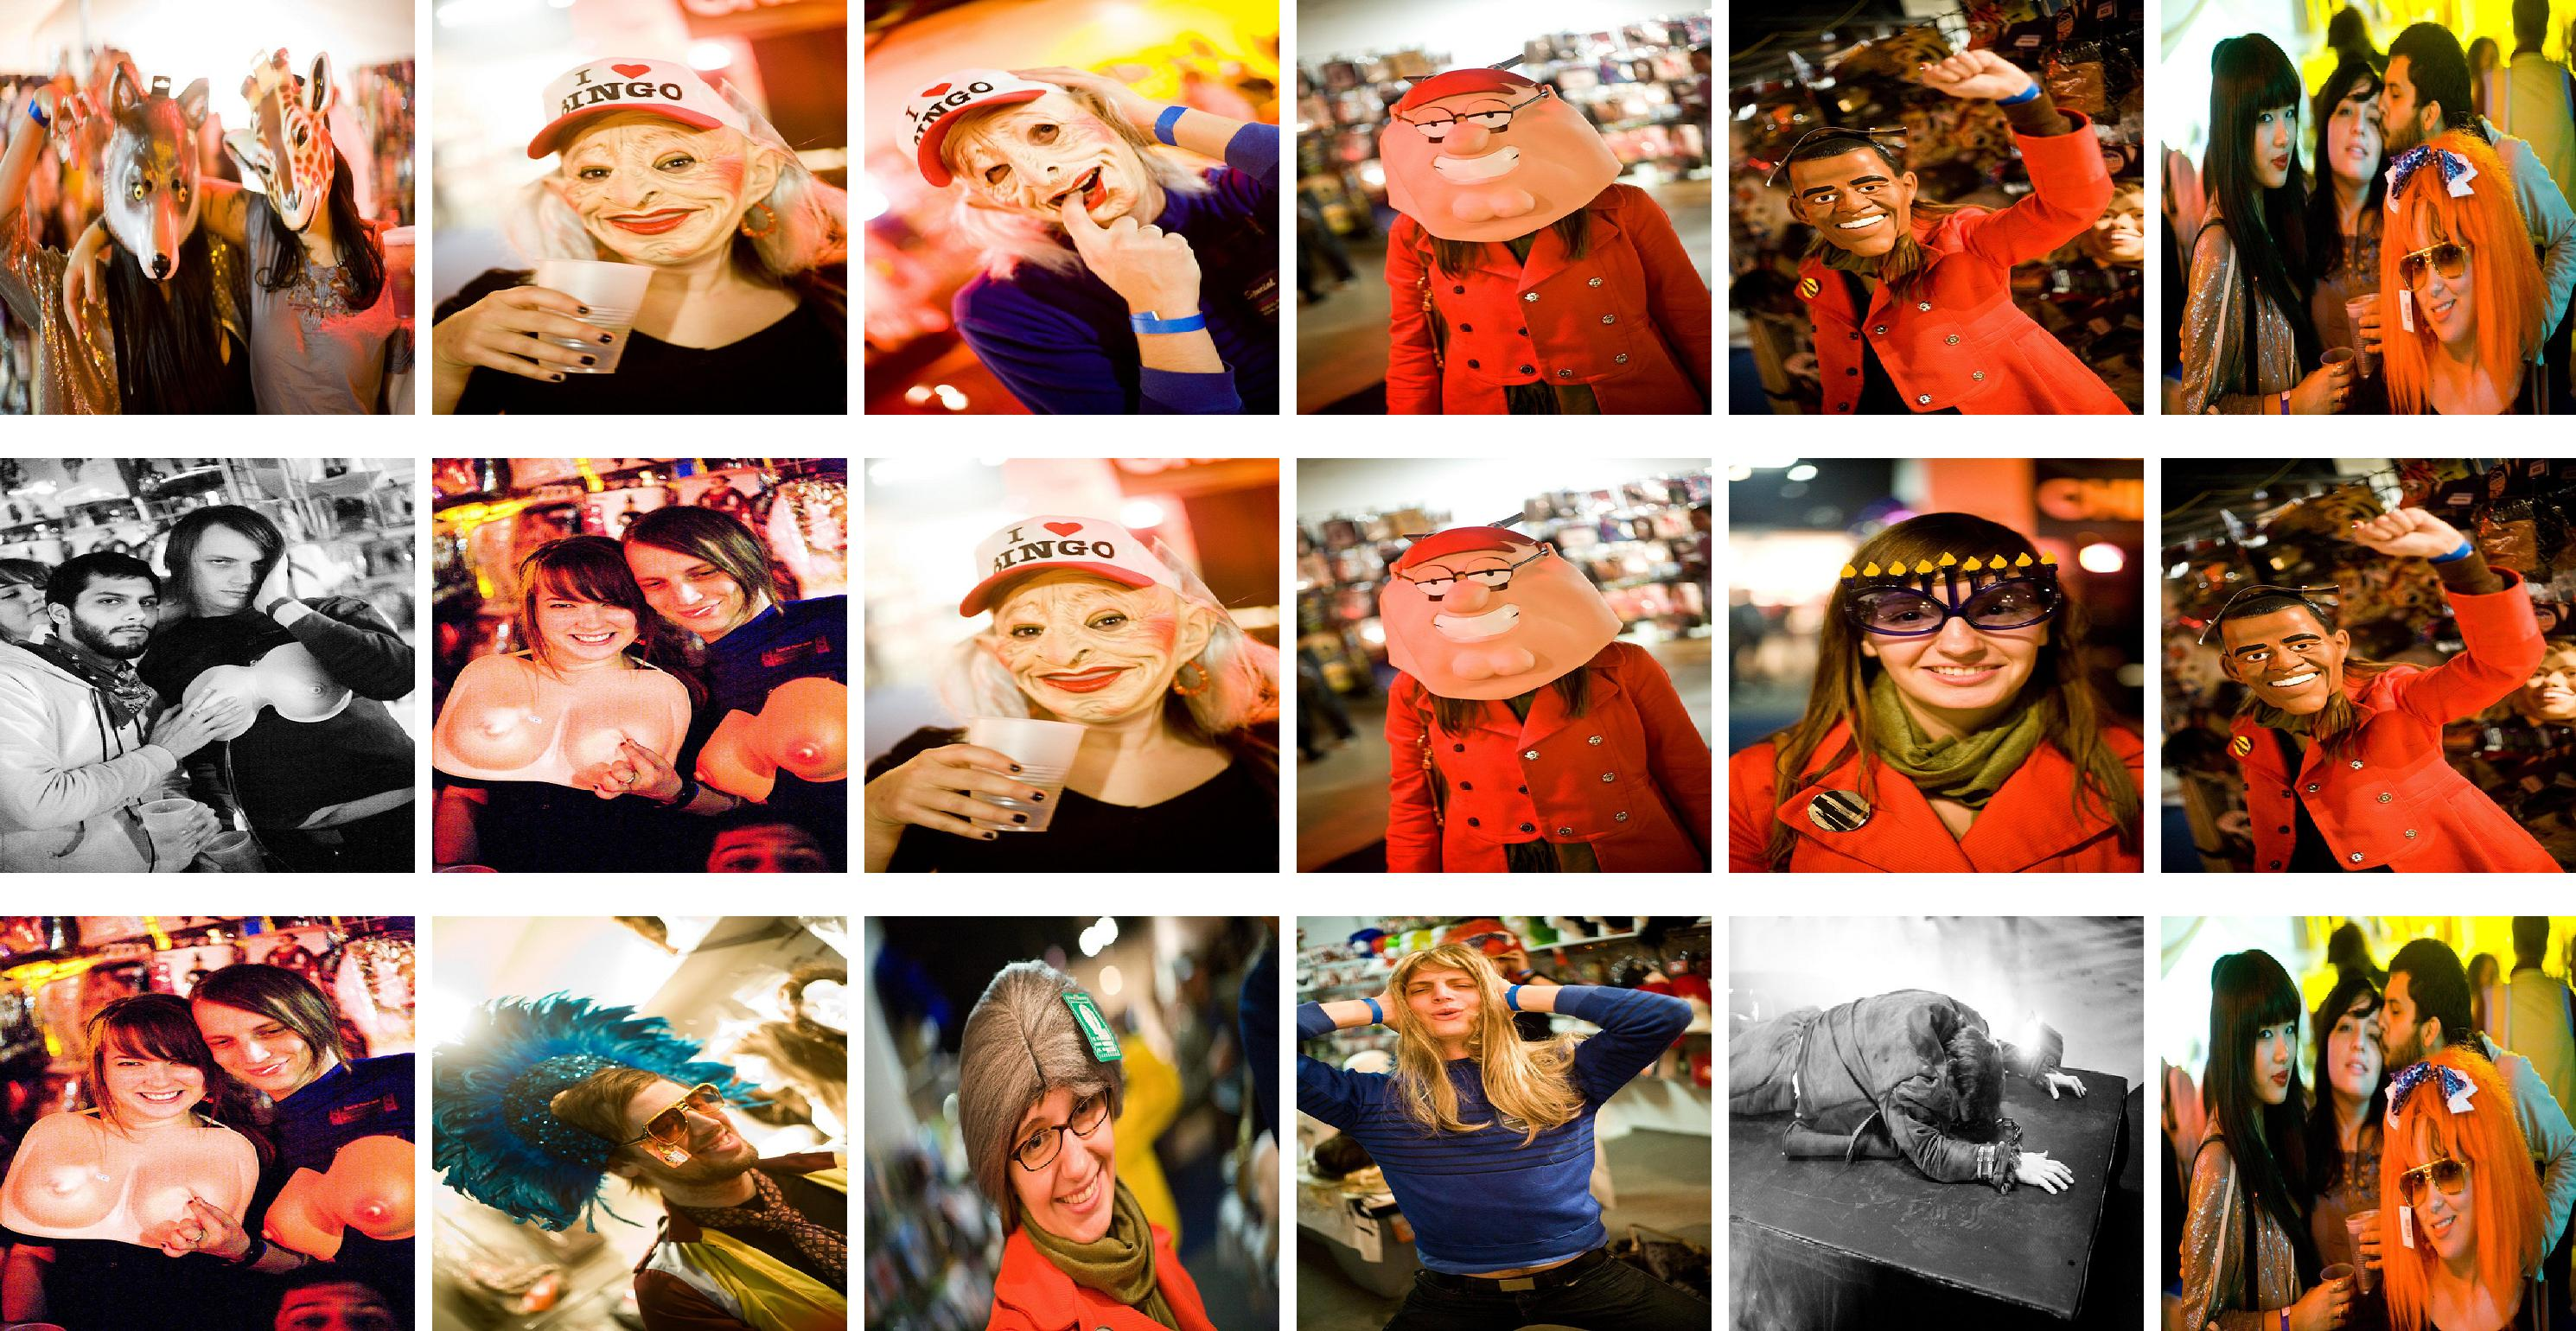
\includegraphics[height=1.5in]{results/a24_0_97681995@N00_6_20.jpg}}
      \subcaptionbox{Top 15\% of a \textit{Graduation} album. \label{fig35}}{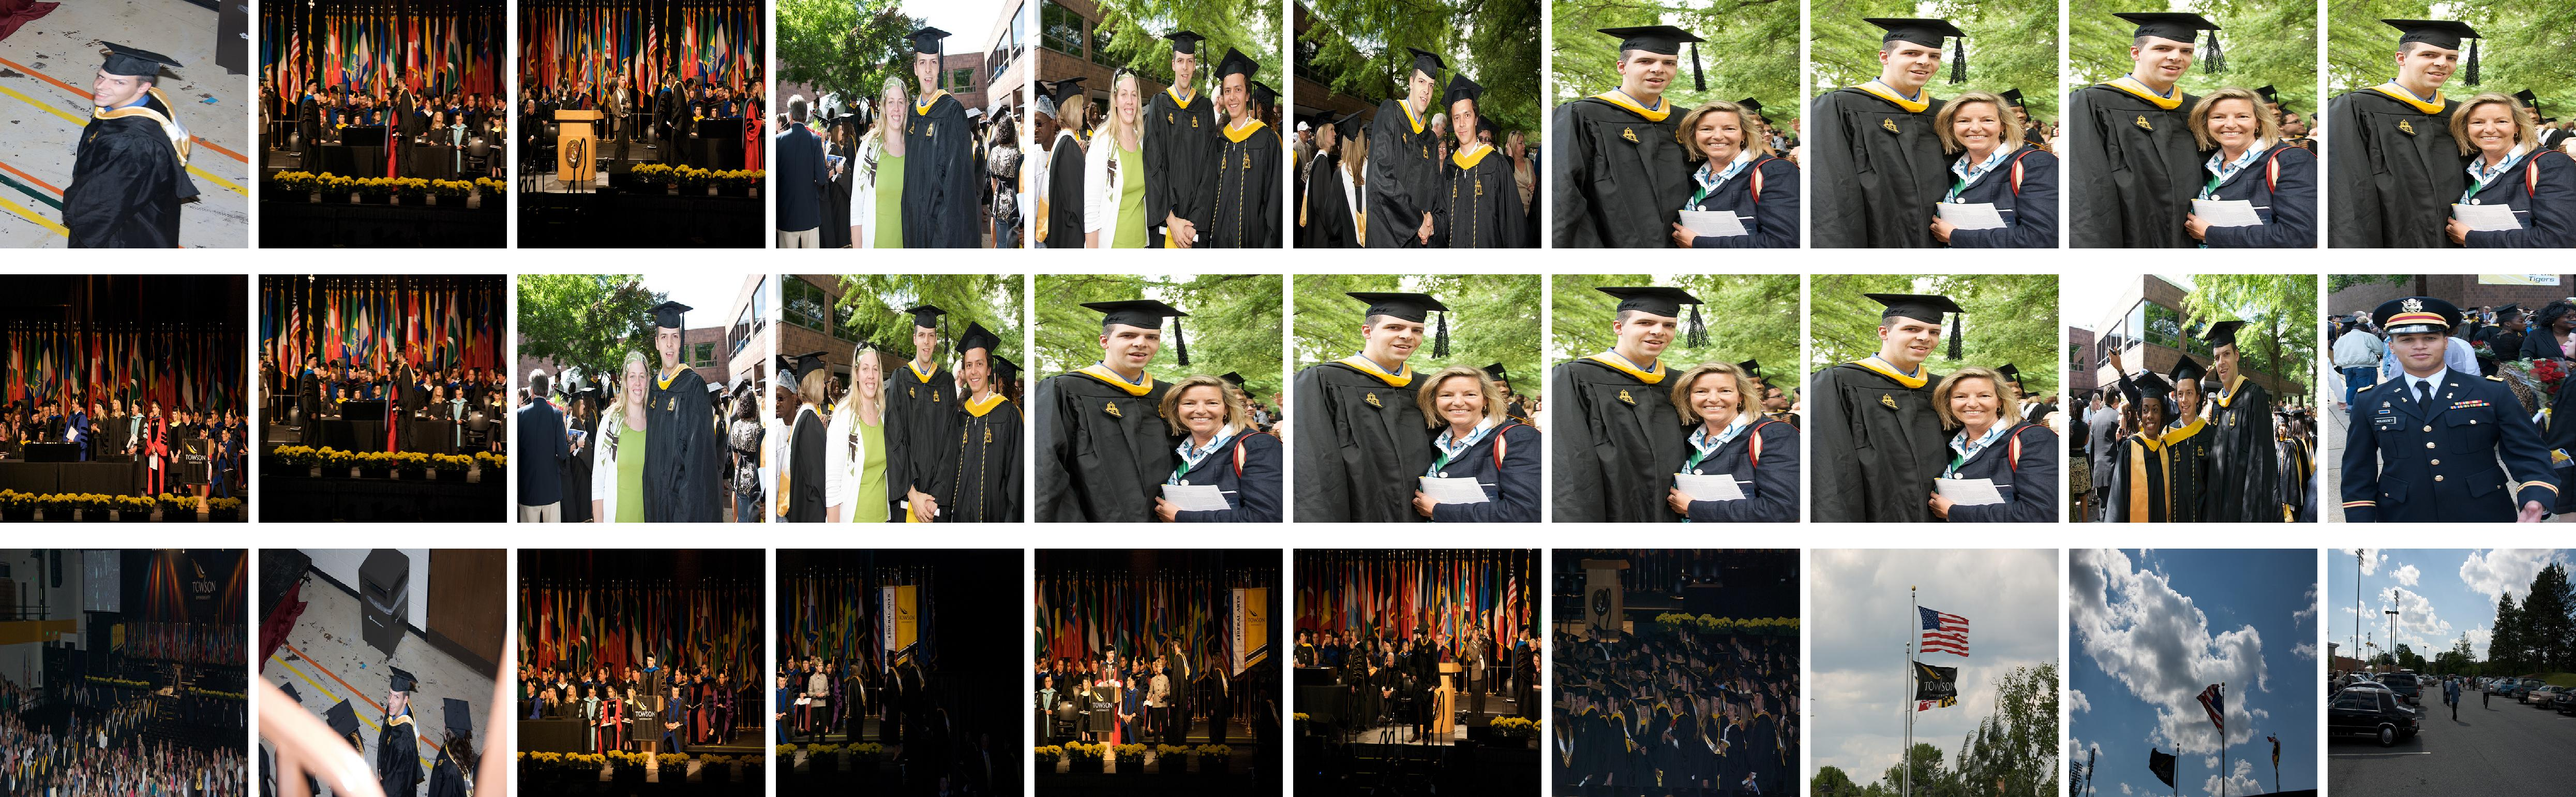
\includegraphics[height=1.5in]{results/a25_25_88483799@N00_10_15.jpg}}
        \subcaptionbox{Top 15\% of a \textit{Urban Trip} album. \label{fig36}}{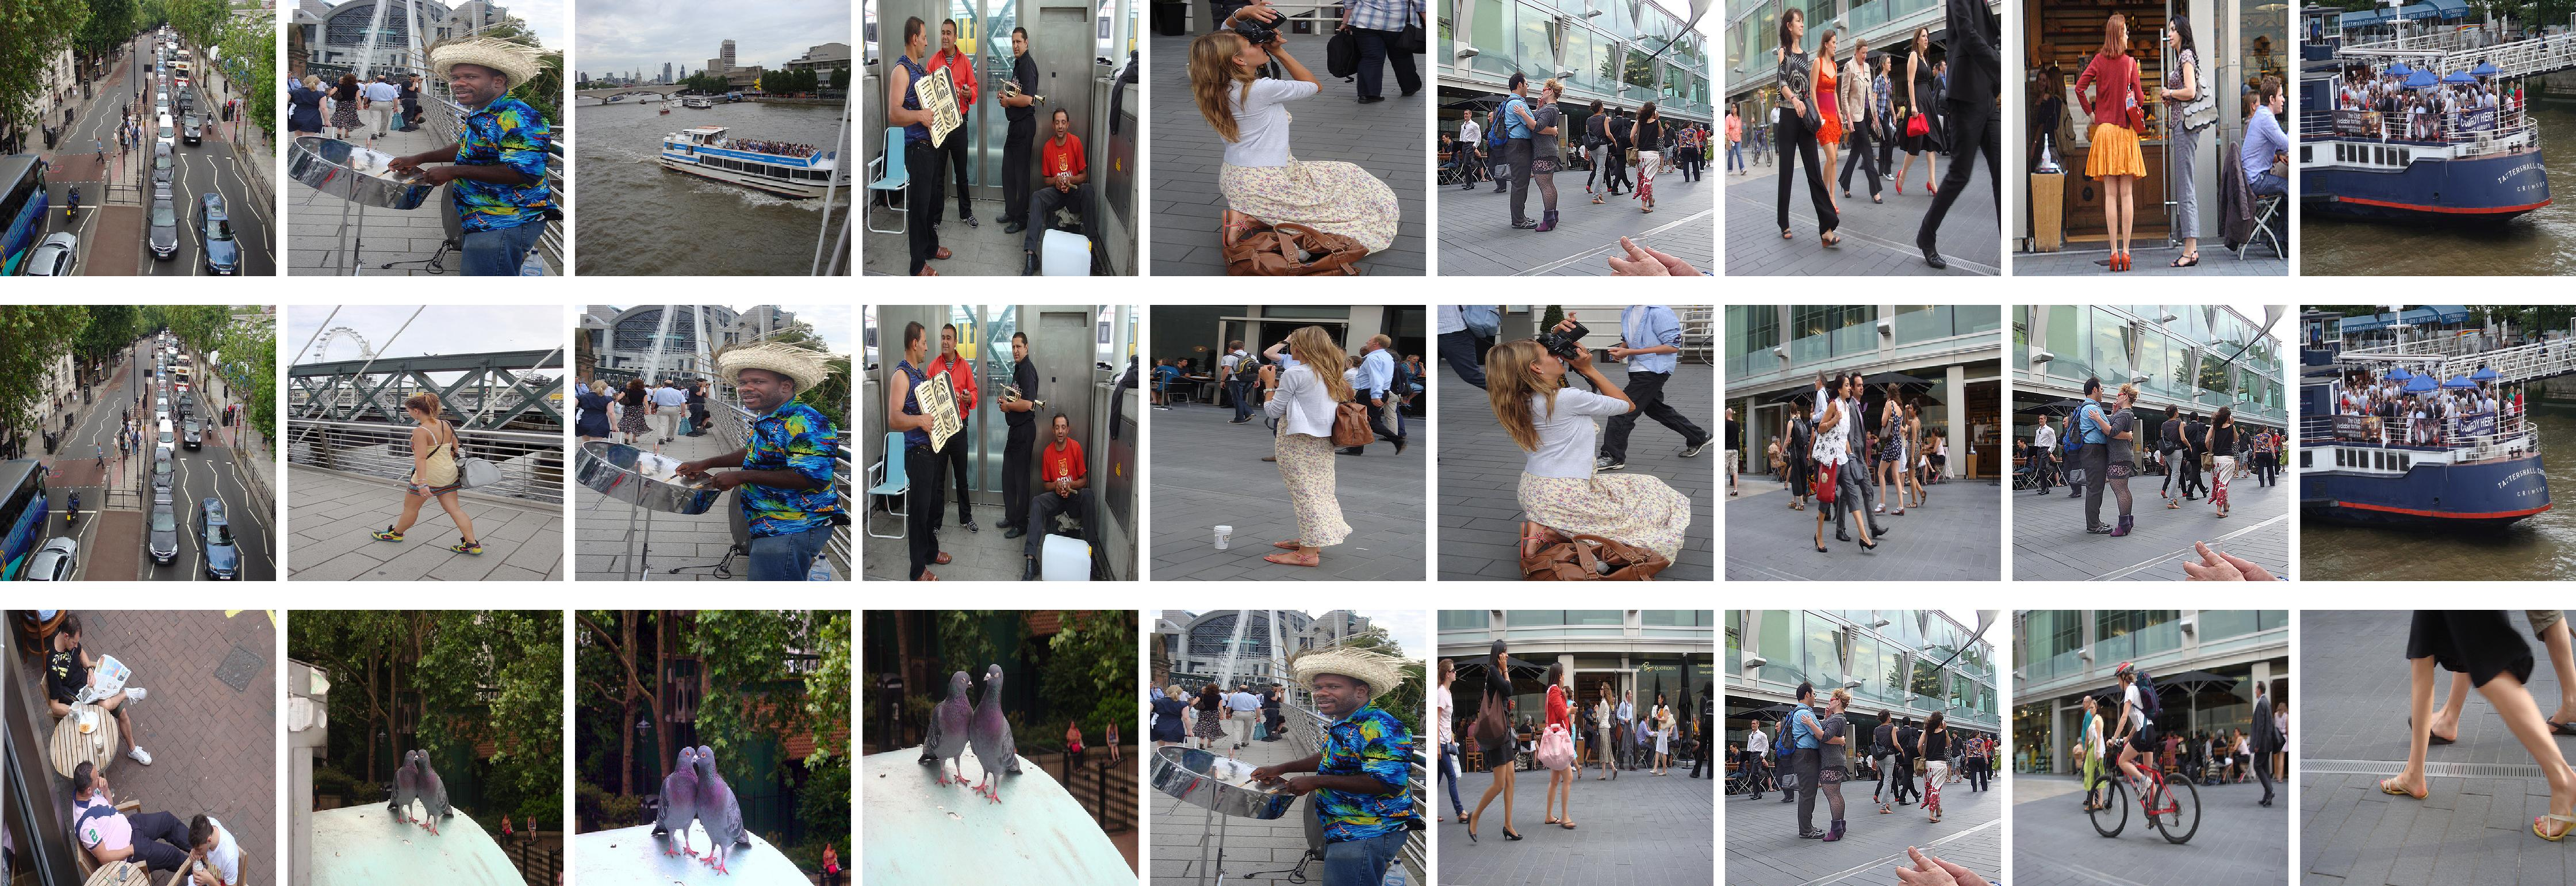
\includegraphics[height=1.5in]{results/a26_97_32323502@N00_9_15.jpg}}
  \caption{Example of results. For each album, top 10-20\% images of the album from three methods are shown. Images are arranged in chronological order. First row is the ground truth we acquired from AMT workers; second row is our prediction using Ensemble-CNN which we introduced in the main paper; third row is the result from random selection.}
  \end{figure*}
  
  \clearpage
  \begin{figure*}[ht]
\centering
  \subcaptionbox{Top 10\% of a \textit{Graduation} album. \label{fig37}}{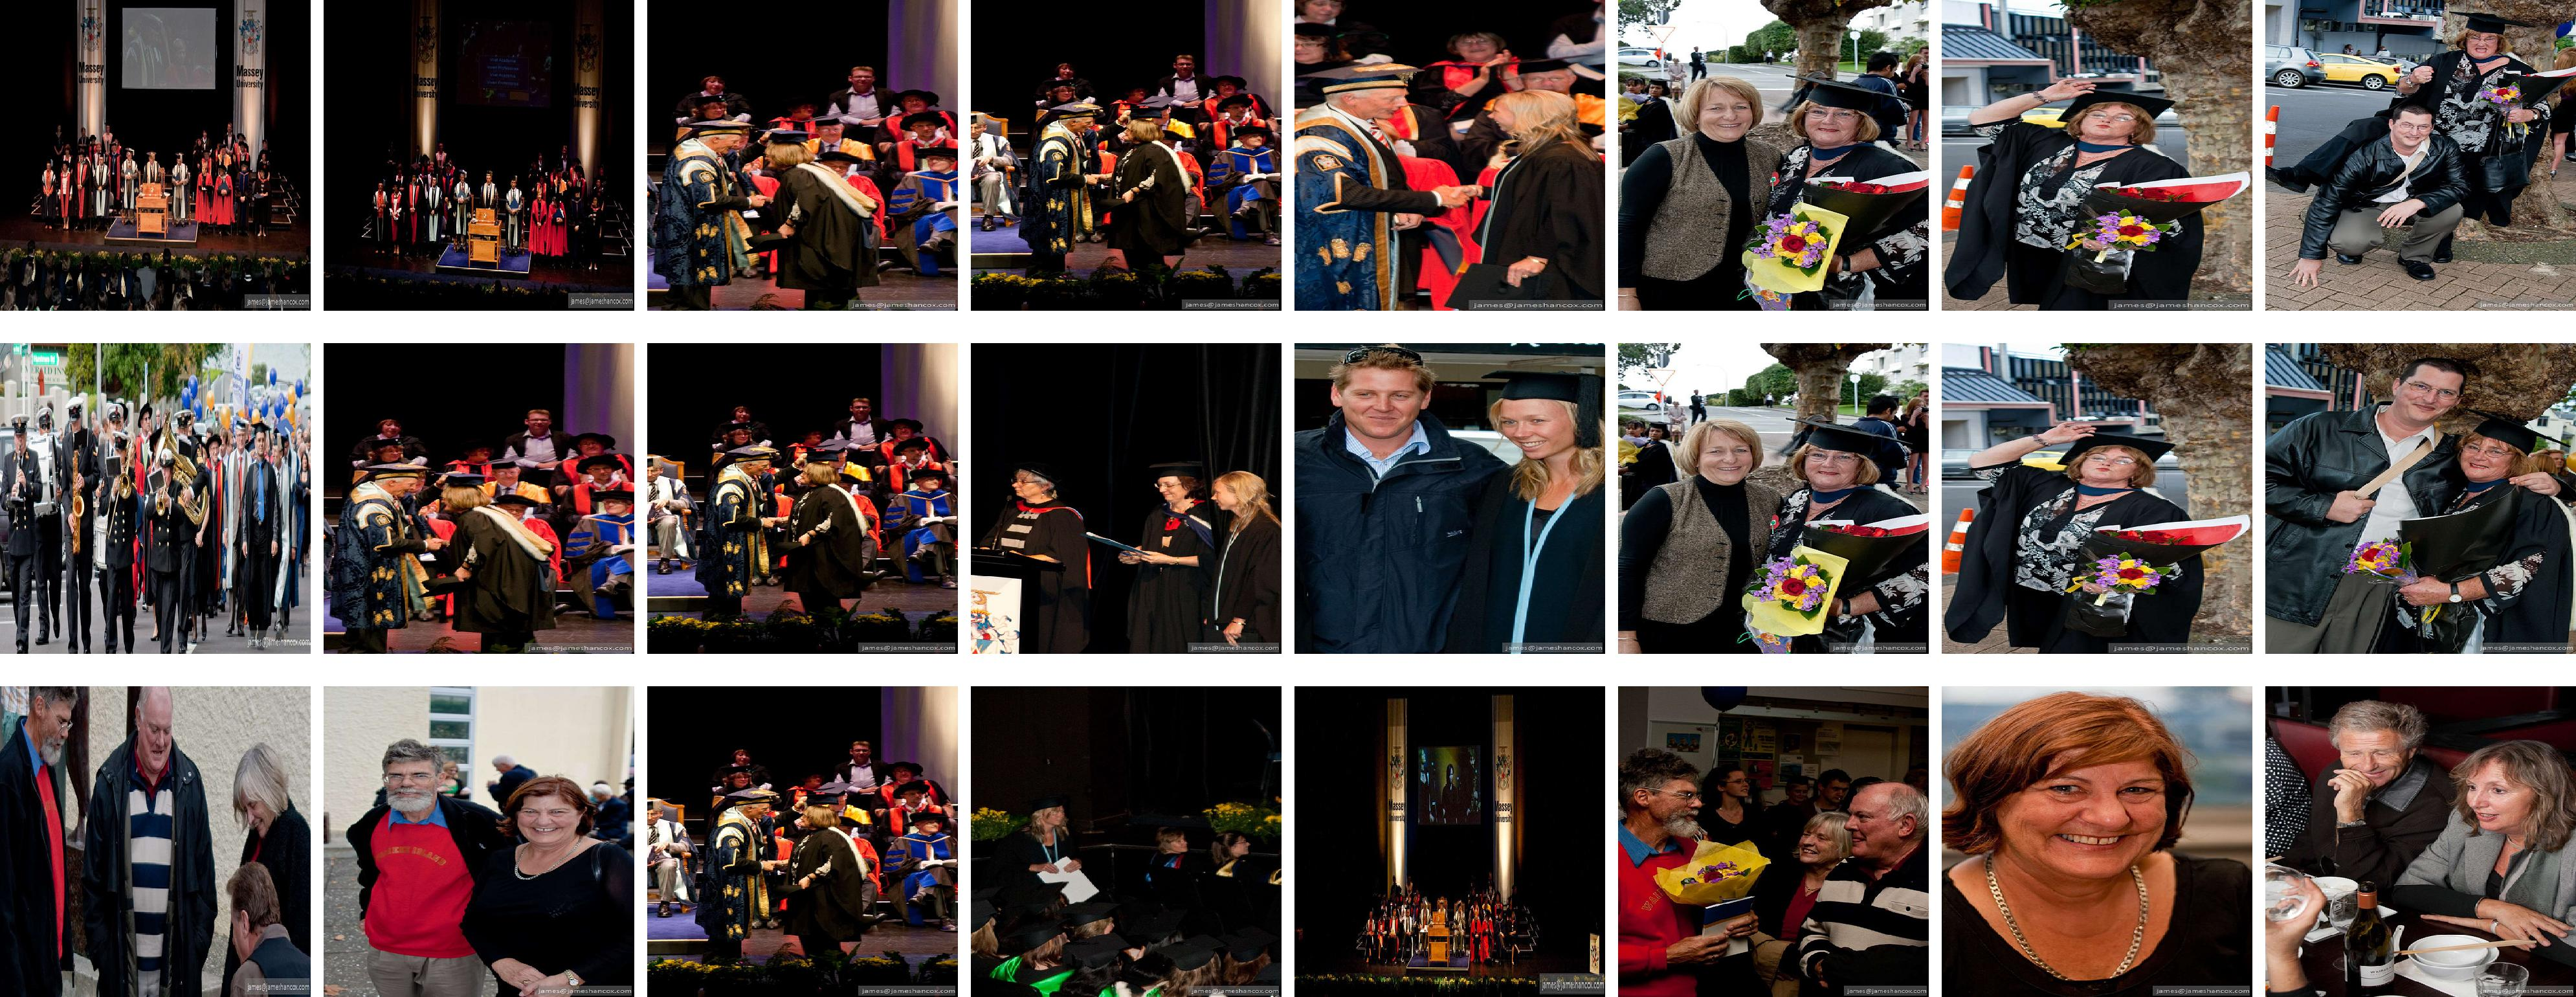
\includegraphics[height=1.5in]{results/b1_2_30275727@N02_8_10.jpg}} \\
  \subcaptionbox{Top 20\% of a \textit{Architecture} album. \label{fig38}}{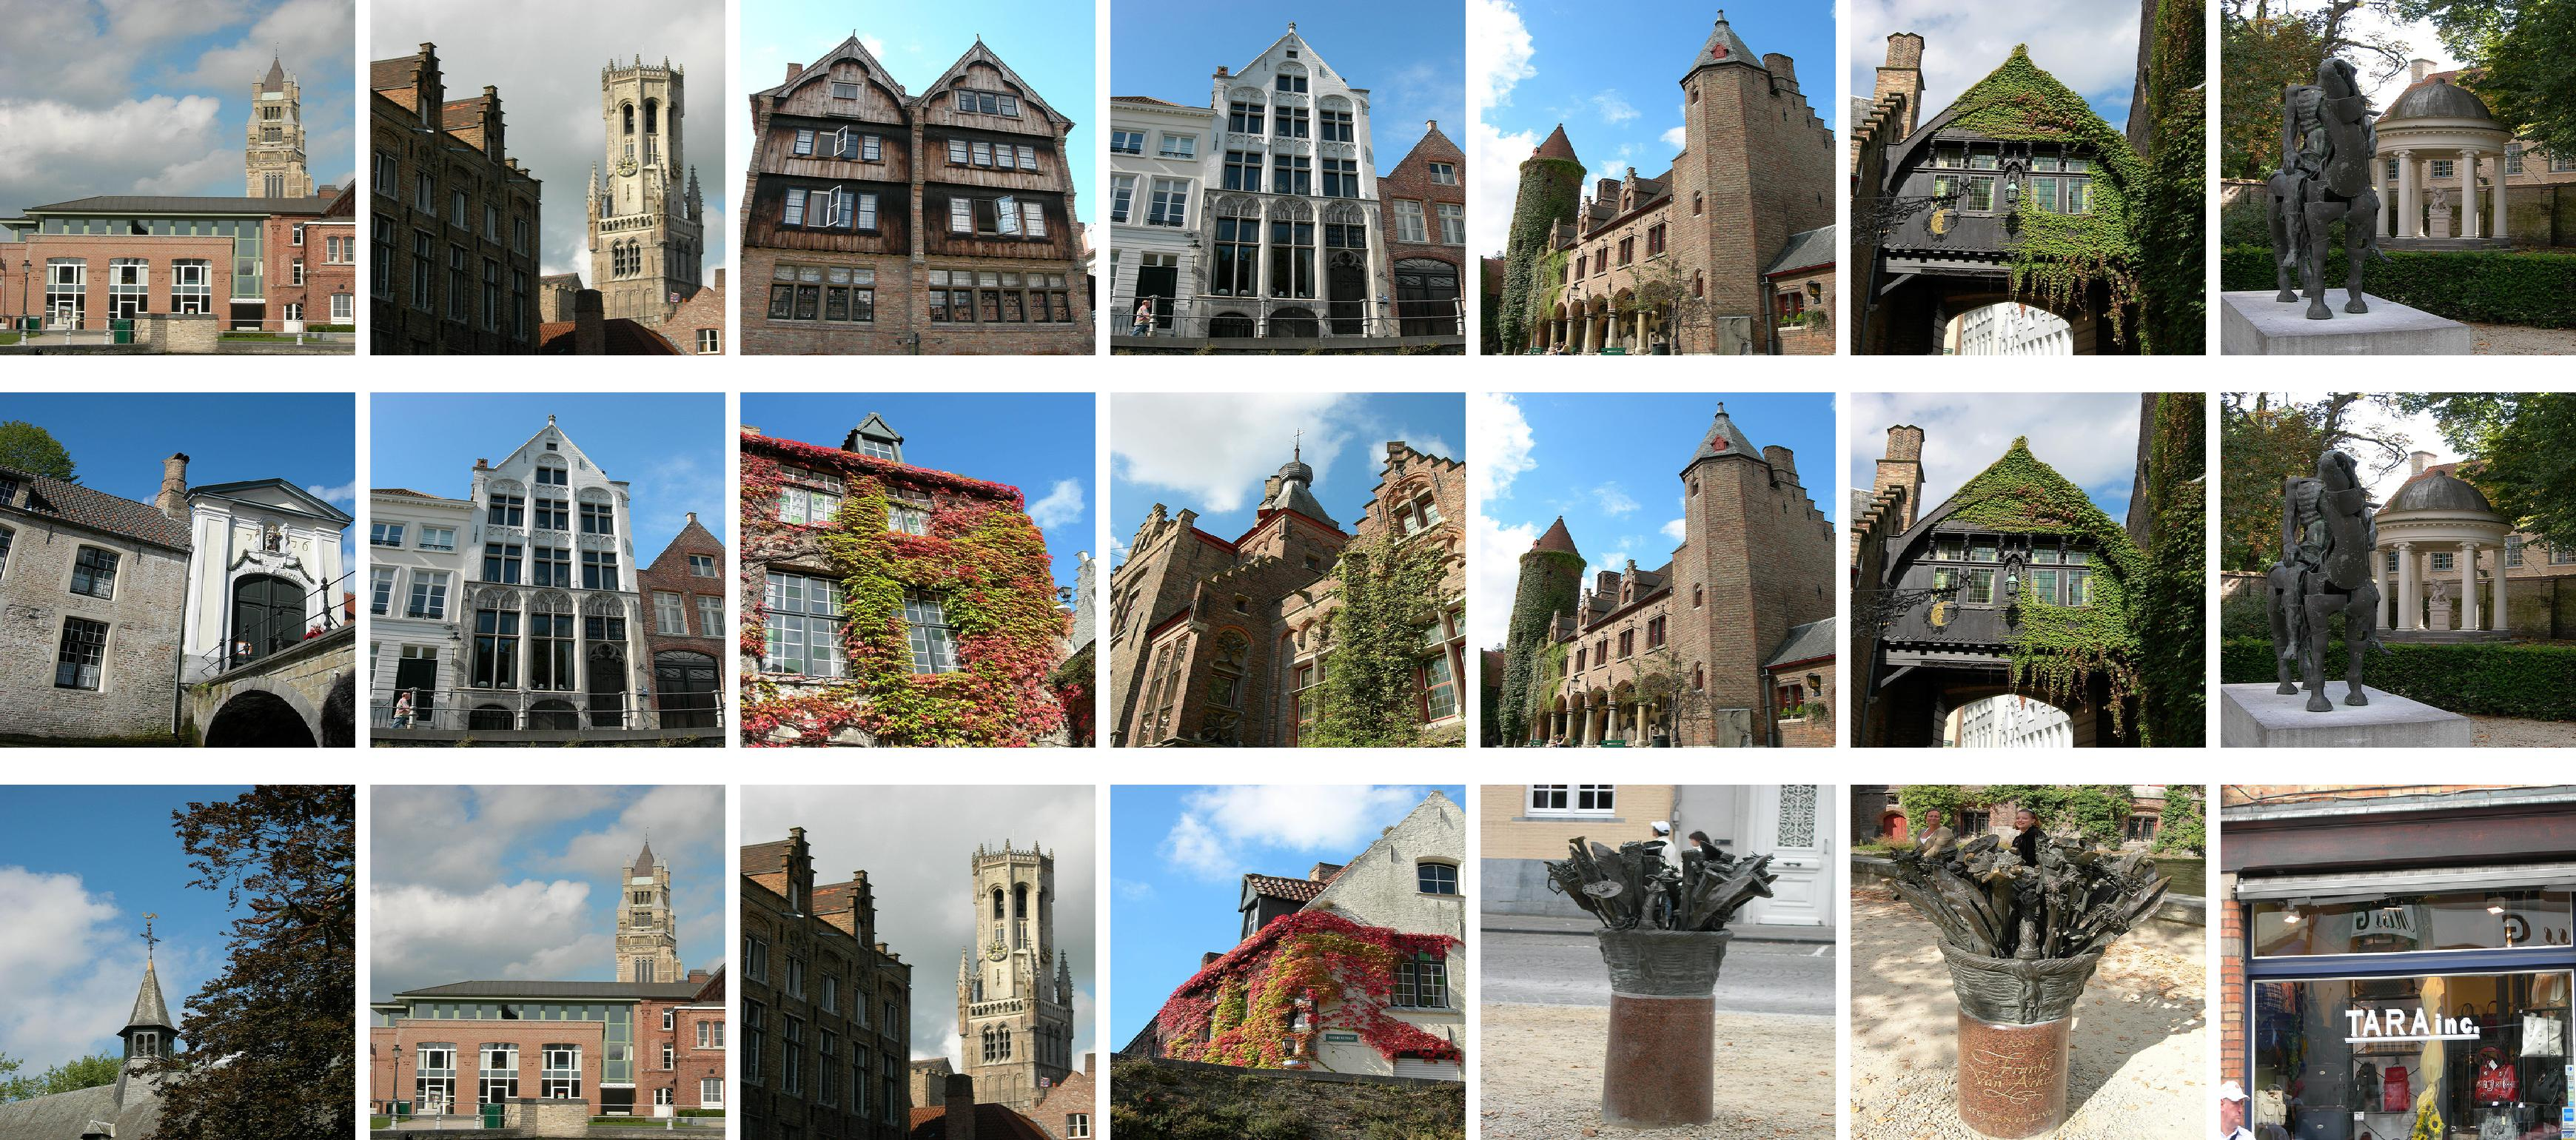
\includegraphics[height=1.5in]{results/b2_2_33237963@N00_7_20.jpg}} \hspace{2em}
  \subcaptionbox{Top 20\% of a \textit{Urban Trip} album. \label{fig39}}{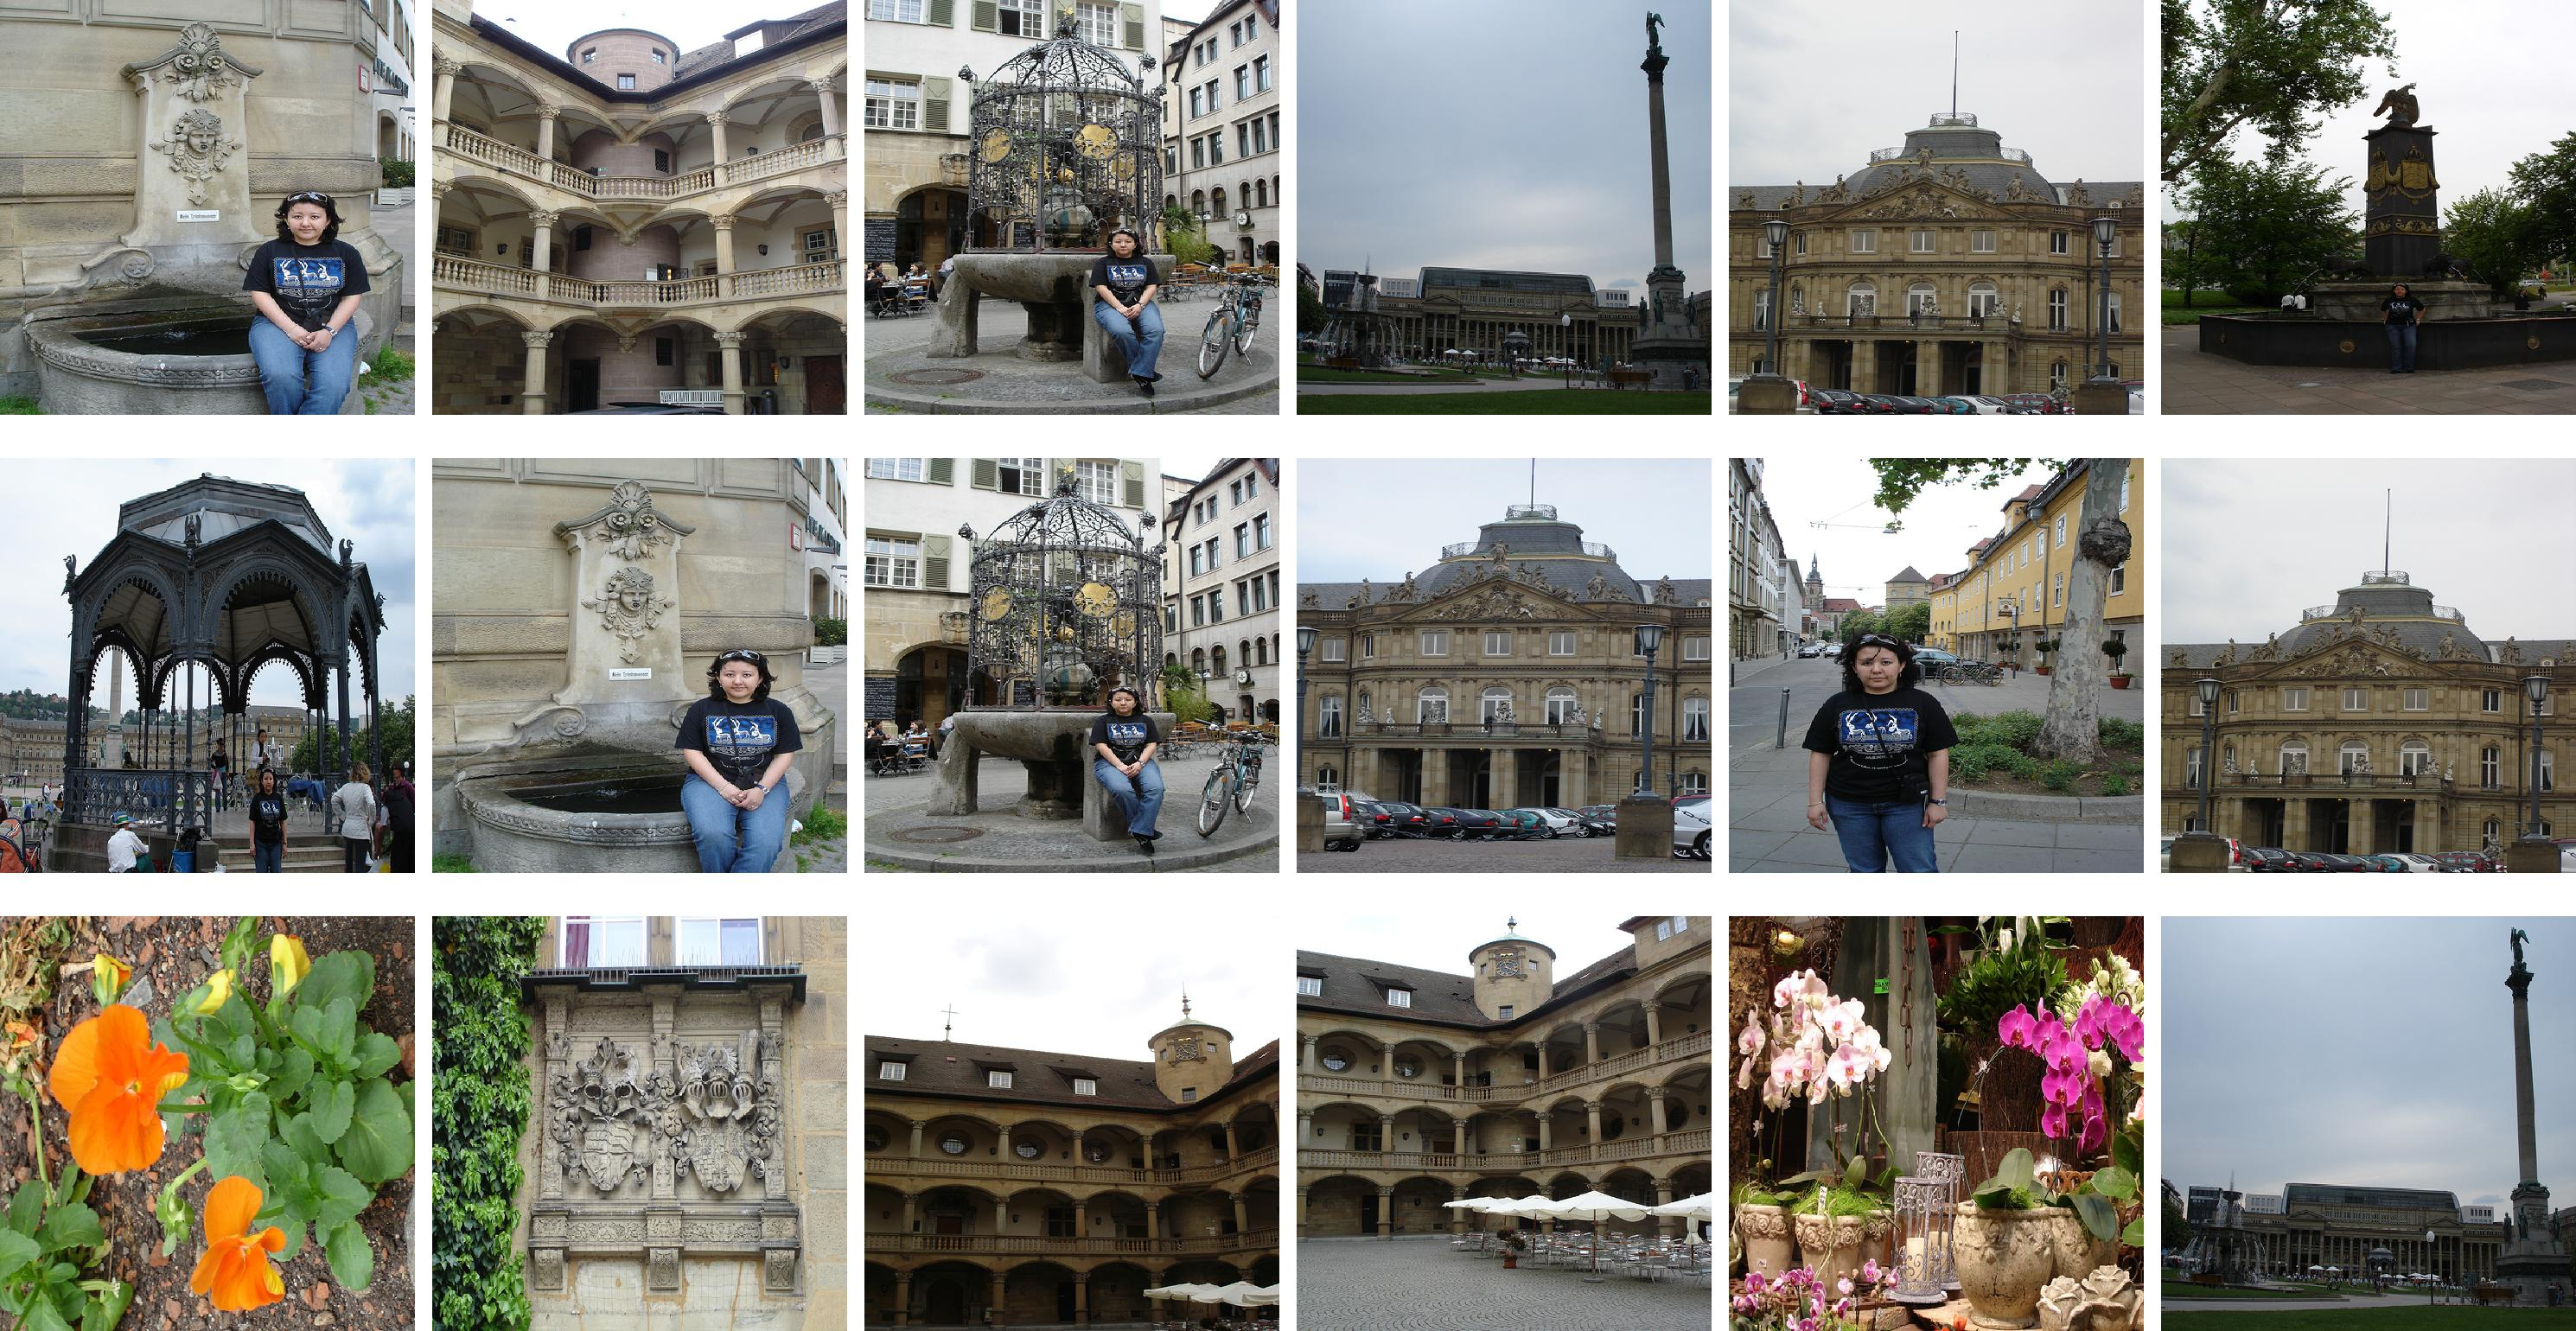
\includegraphics[height=1.5in]{results/b3_2_96212491@N00_6_20.jpg}} 
  \subcaptionbox{Top 20\% of a \textit{Business Activity} album. \label{fig40}}{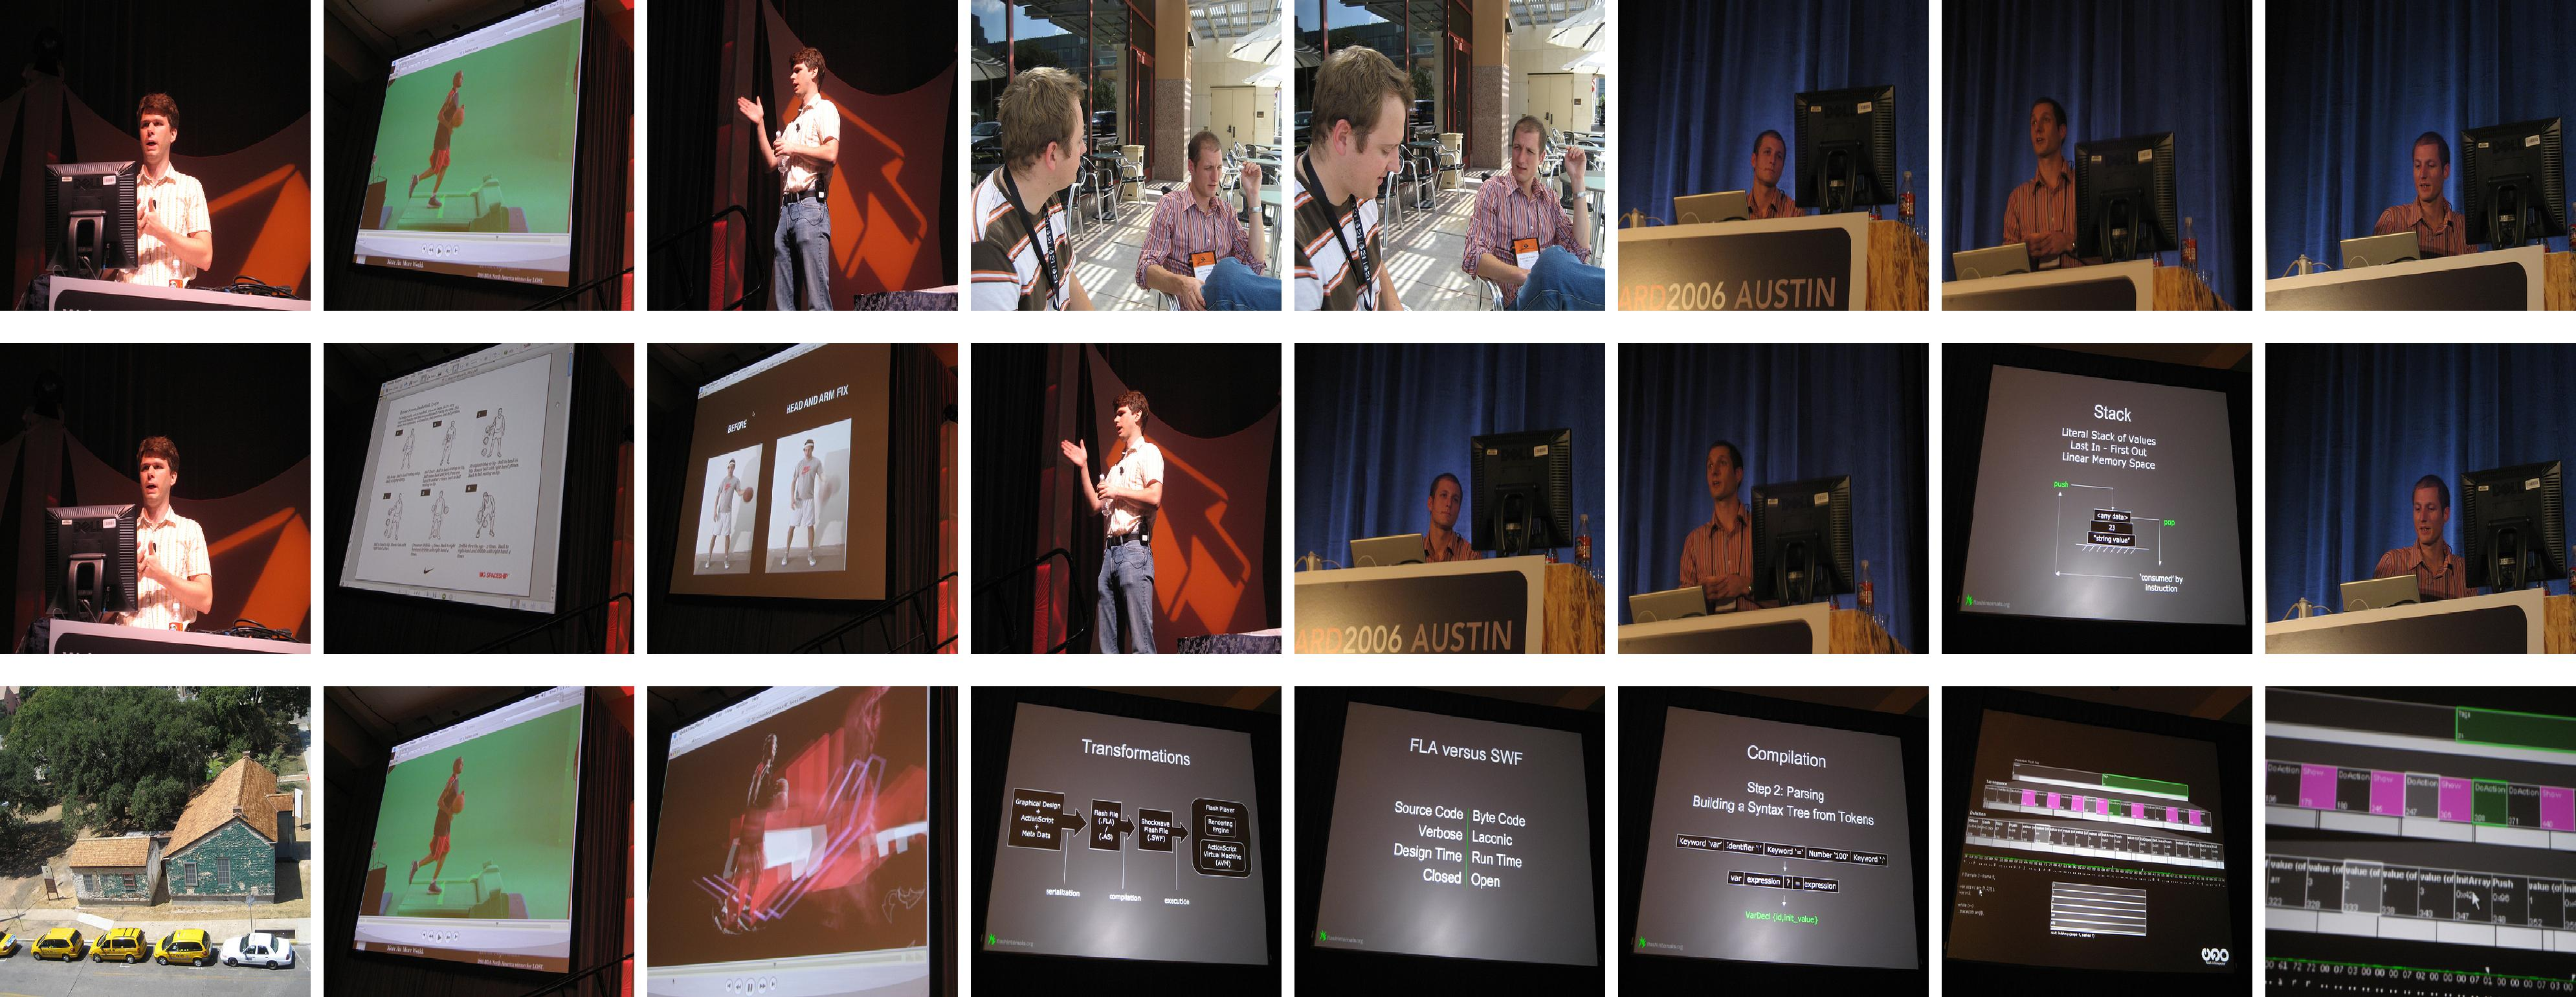
\includegraphics[height=1.5in]{results/b4_0_68598987@N00_8_20.jpg}}
  \subcaptionbox{Top 20\% of a \textit{Business Activity} album. \label{fig41}}{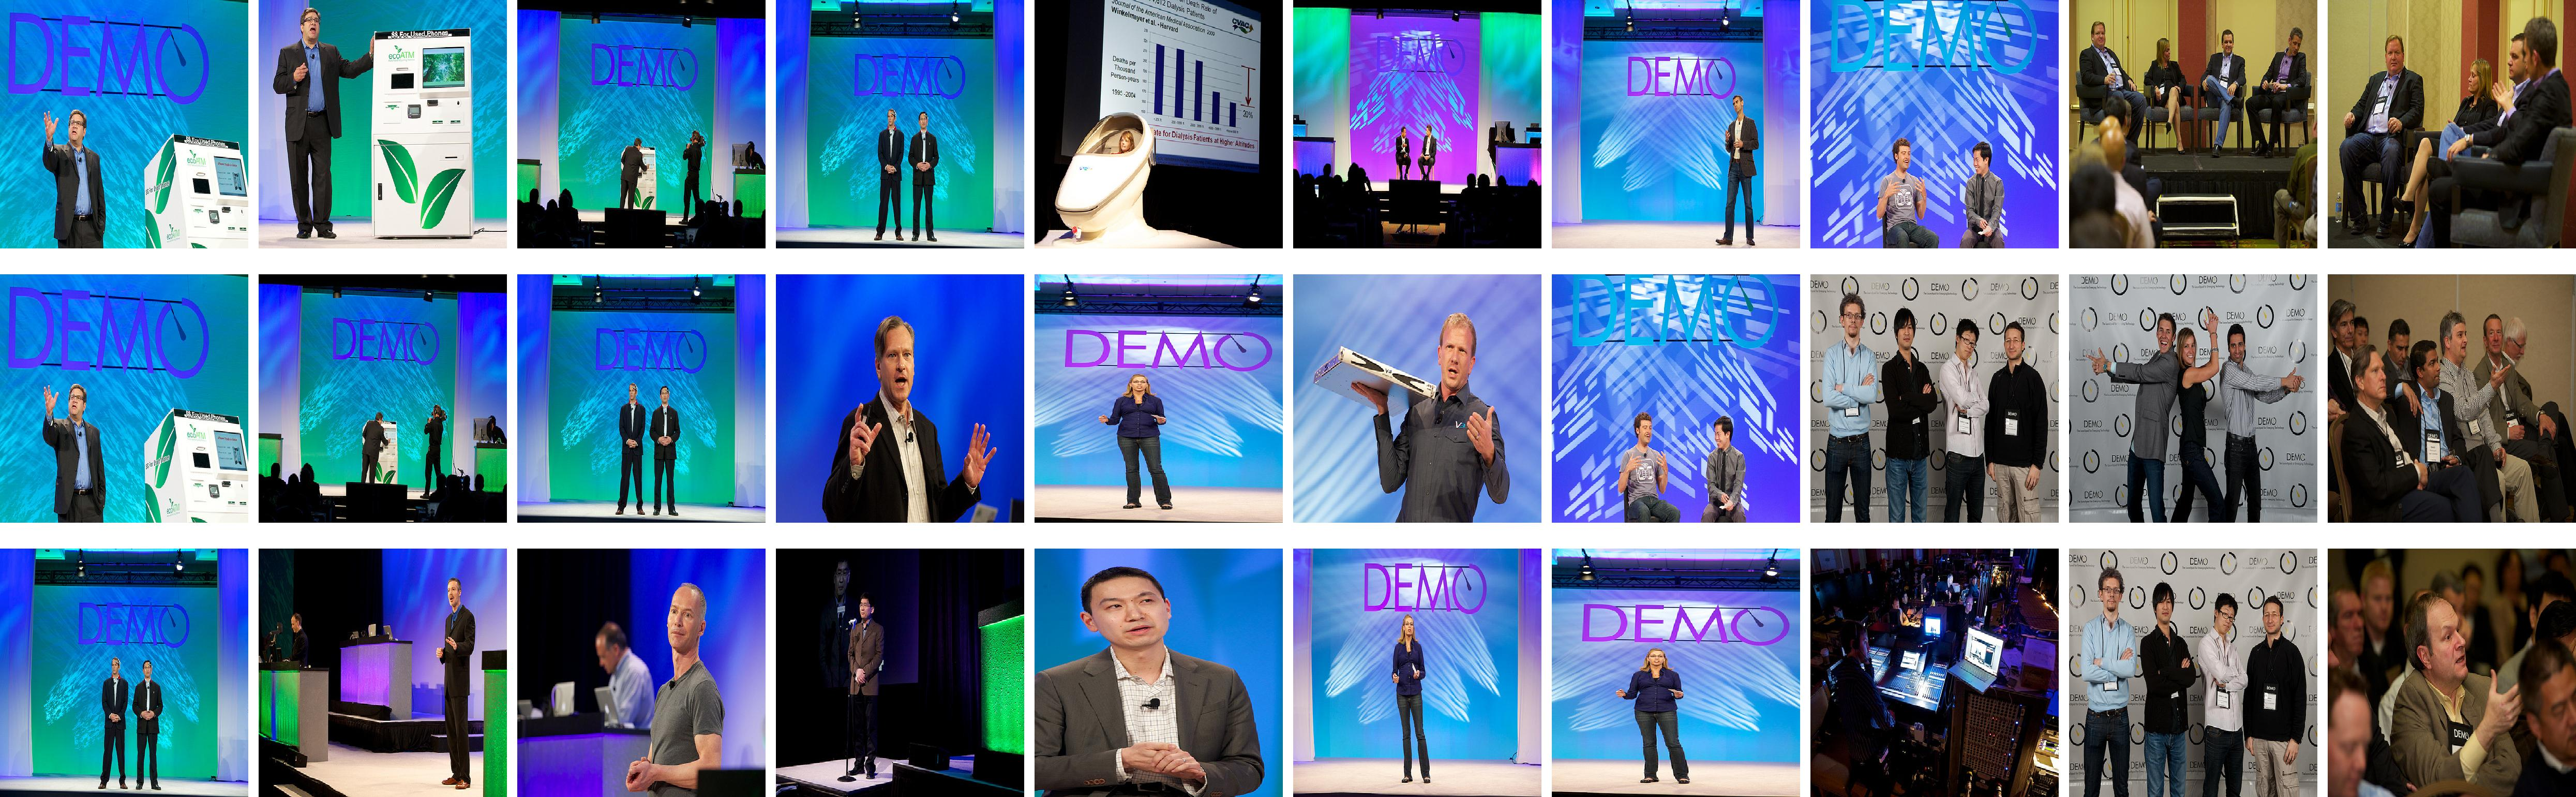
\includegraphics[height=1.5in]{results/b5_3_9025932@N08_10_20.jpg}} \hspace{2em}
    \subcaptionbox{Top 20\% of a \textit{Wedding} album. \label{fig42}}{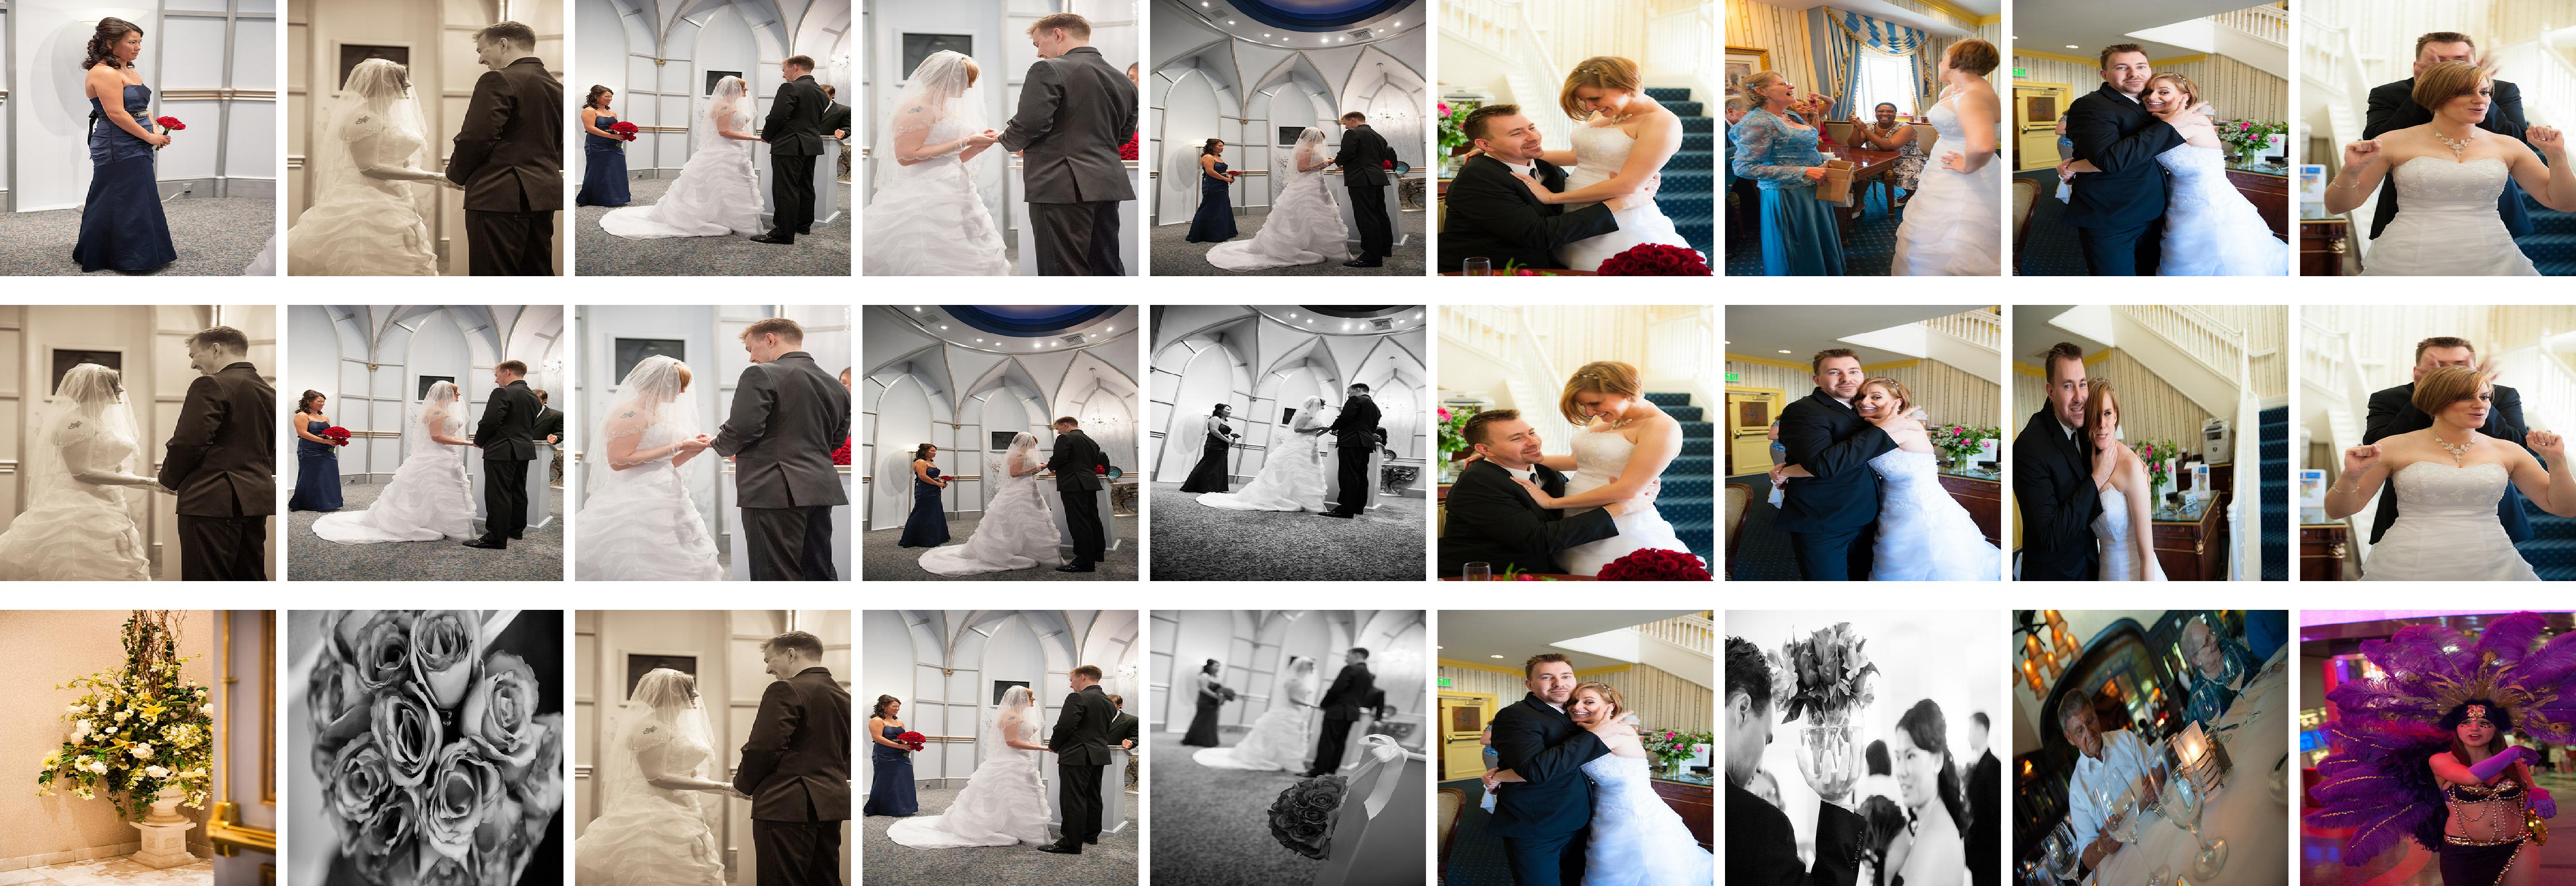
\includegraphics[height=1.5in]{results/b6_3_82373898@N00_9_20.jpg}}
      \end{figure*}
        
  \clearpage
  \begin{figure*}[ht]
  \ContinuedFloat % continue from previous page
\centering
      \subcaptionbox{Top 10\% of a \textit{Graduation} album. \label{fig43}}{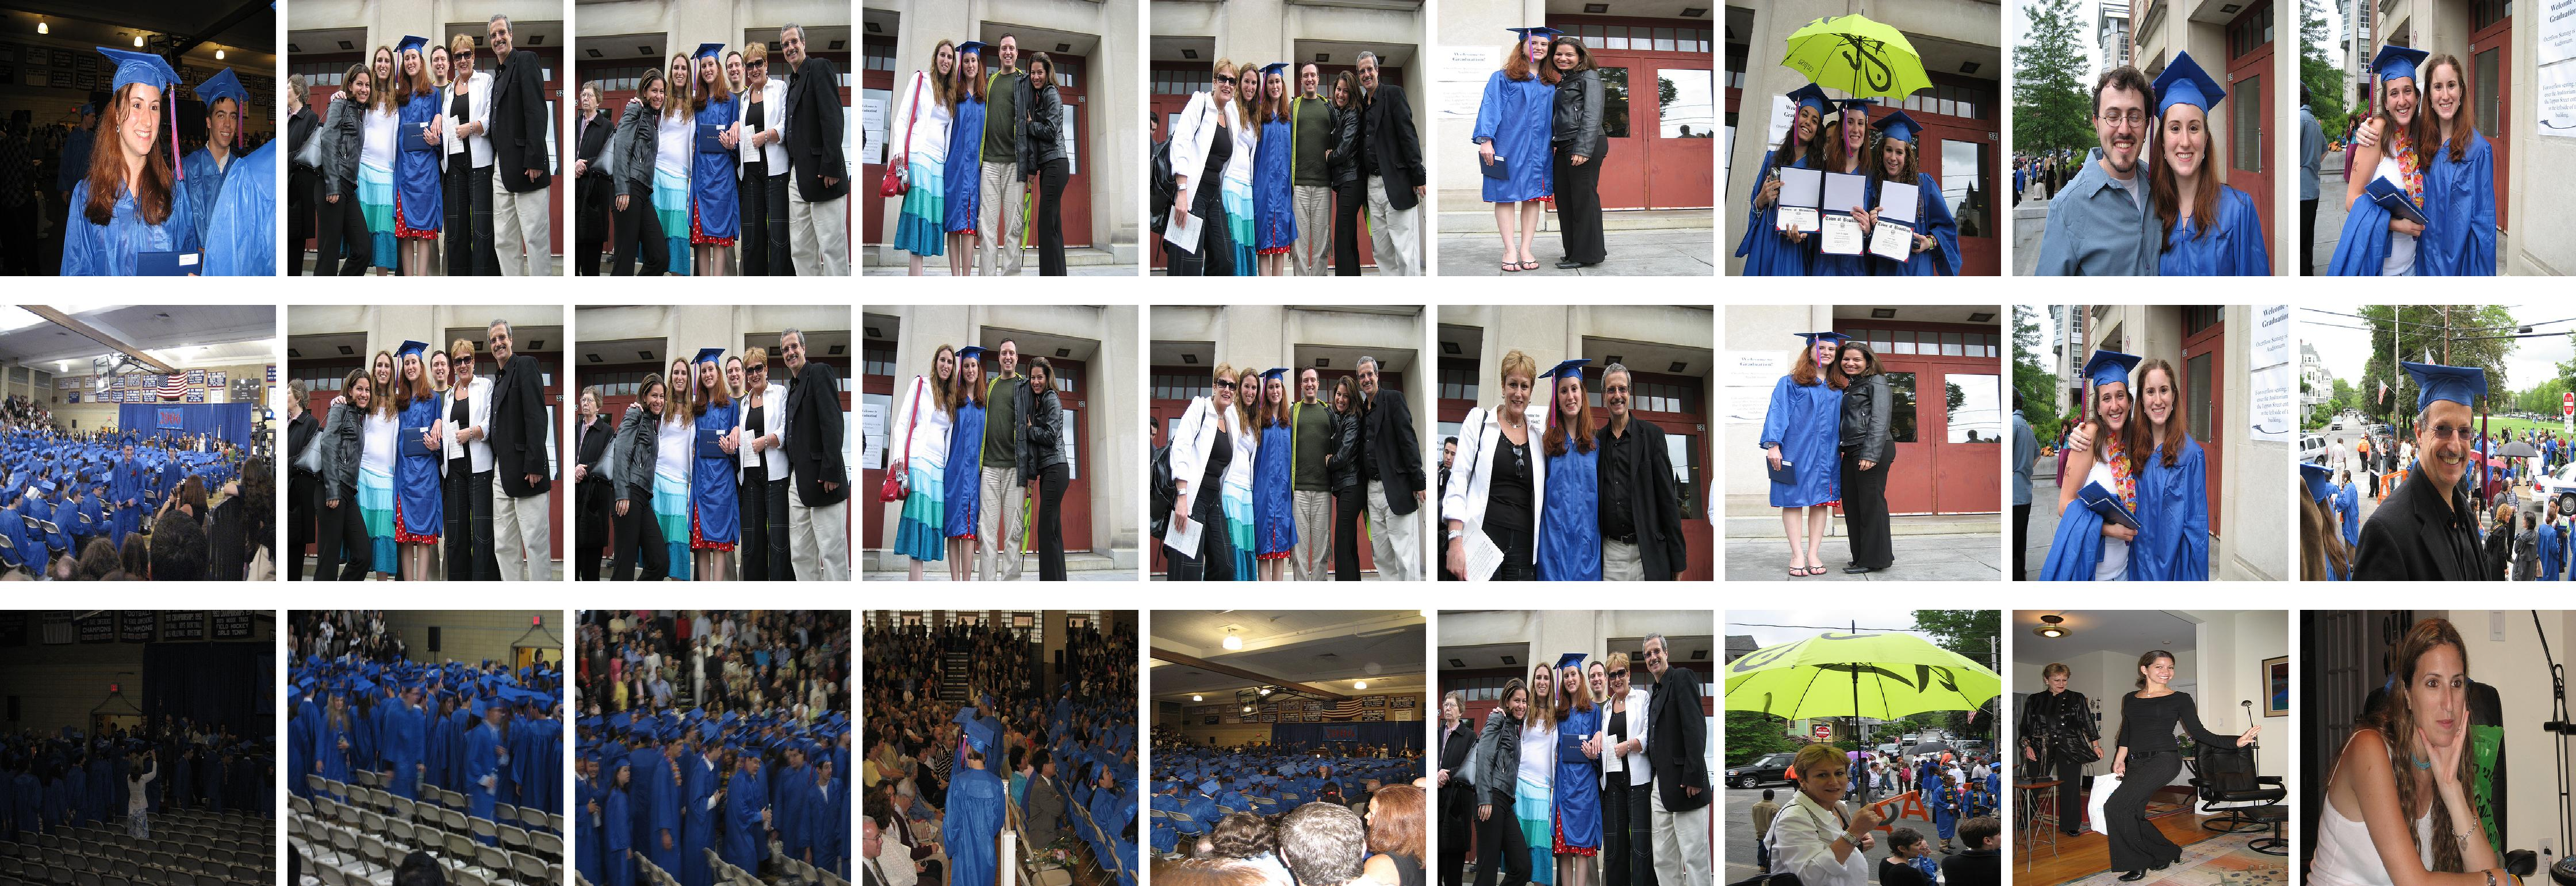
\includegraphics[height=1.5in]{results/b7_4_49561754@N00_9_10.jpg}}
     \subcaptionbox{Top 20\% of a \textit{Birthday} album. \label{fig44}}{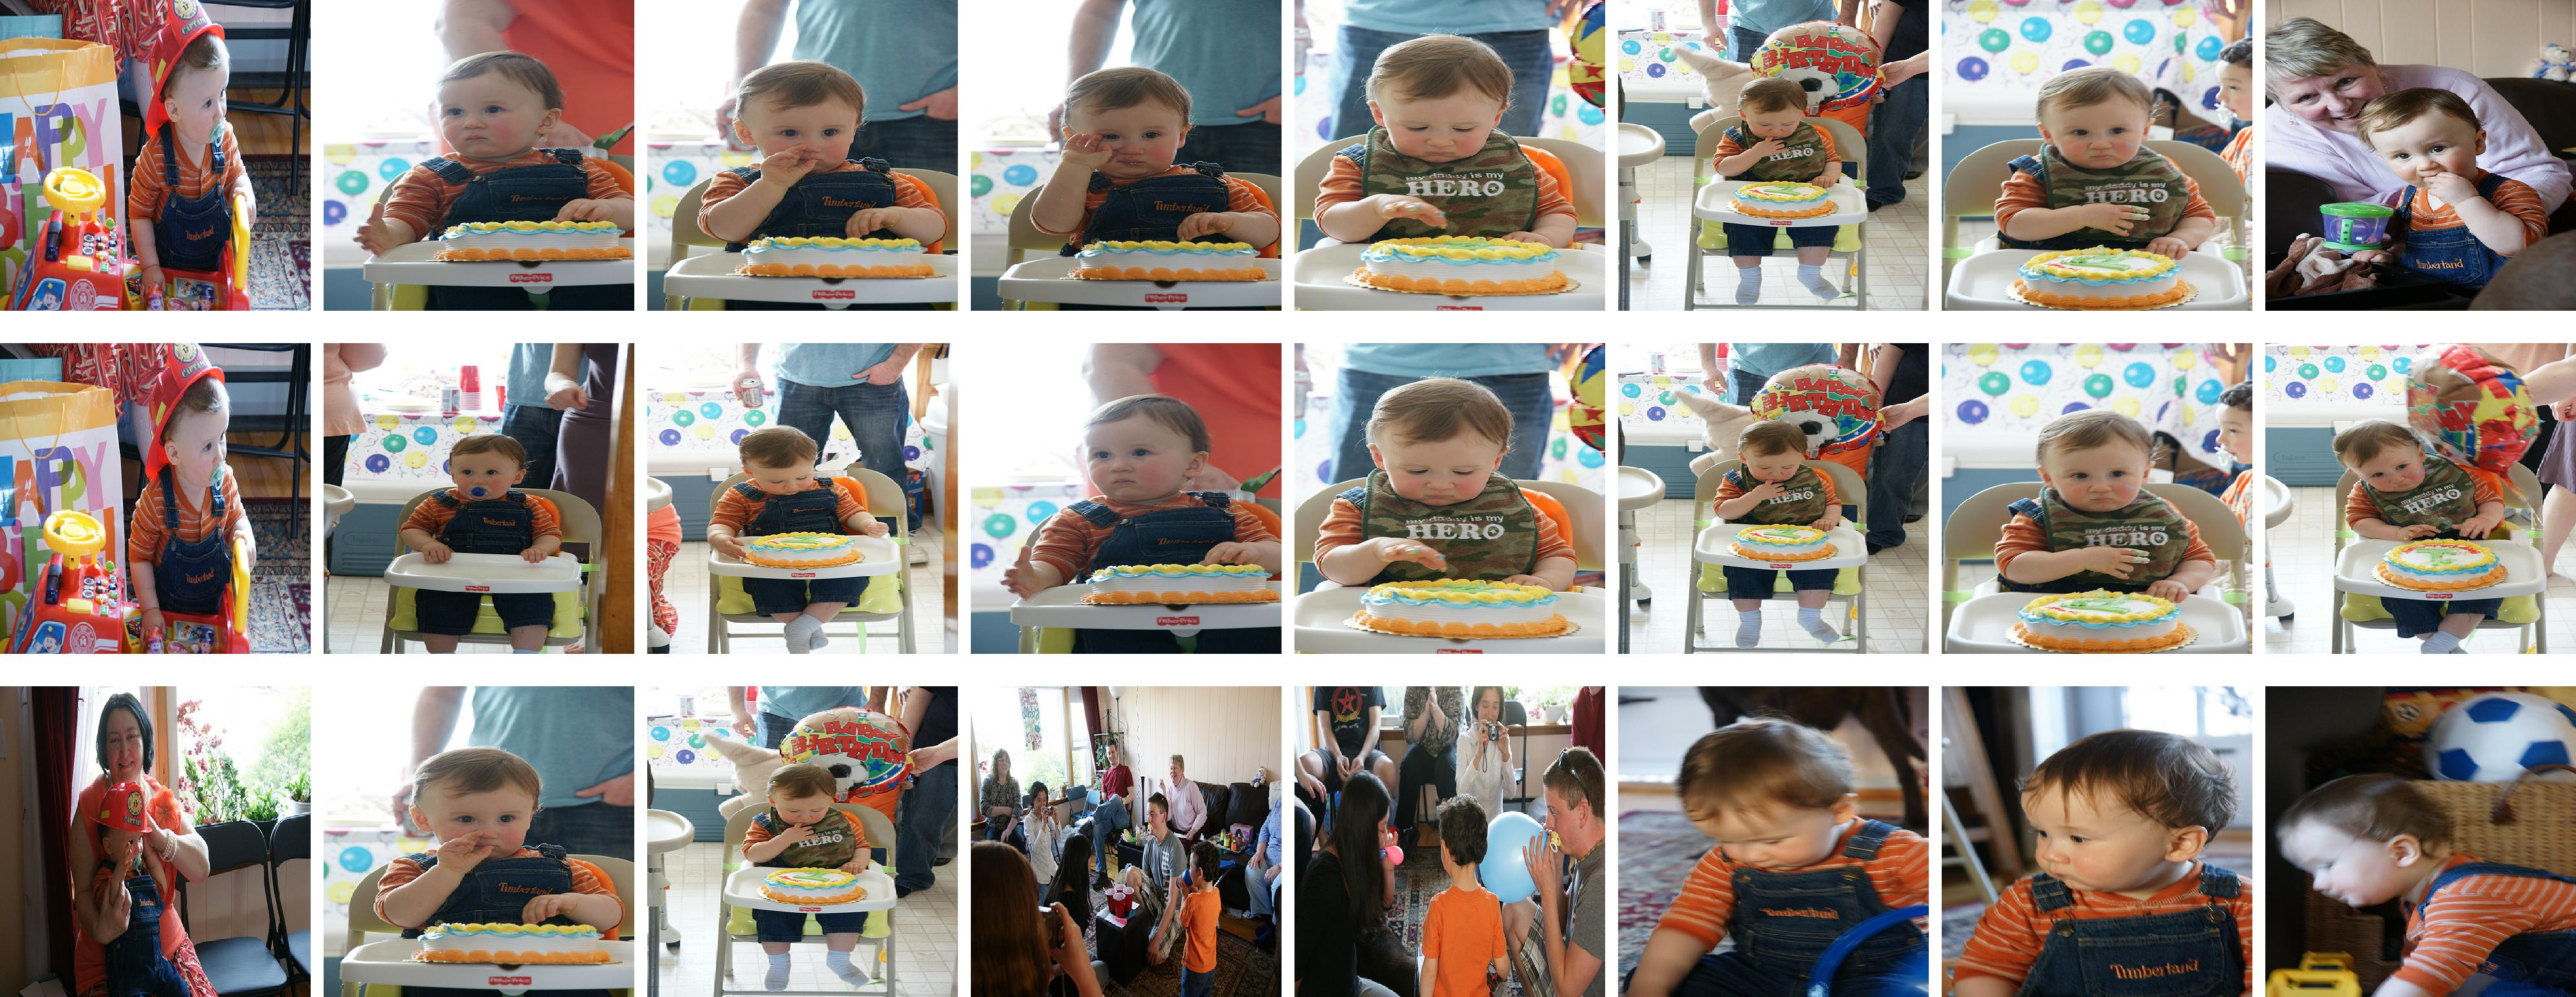
\includegraphics[height=1.5in]{results/b8_6_93995264@N00_8_20.jpg}}
     \subcaptionbox{Top 20\% of a \textit{Architecture} album. \label{fig45}}{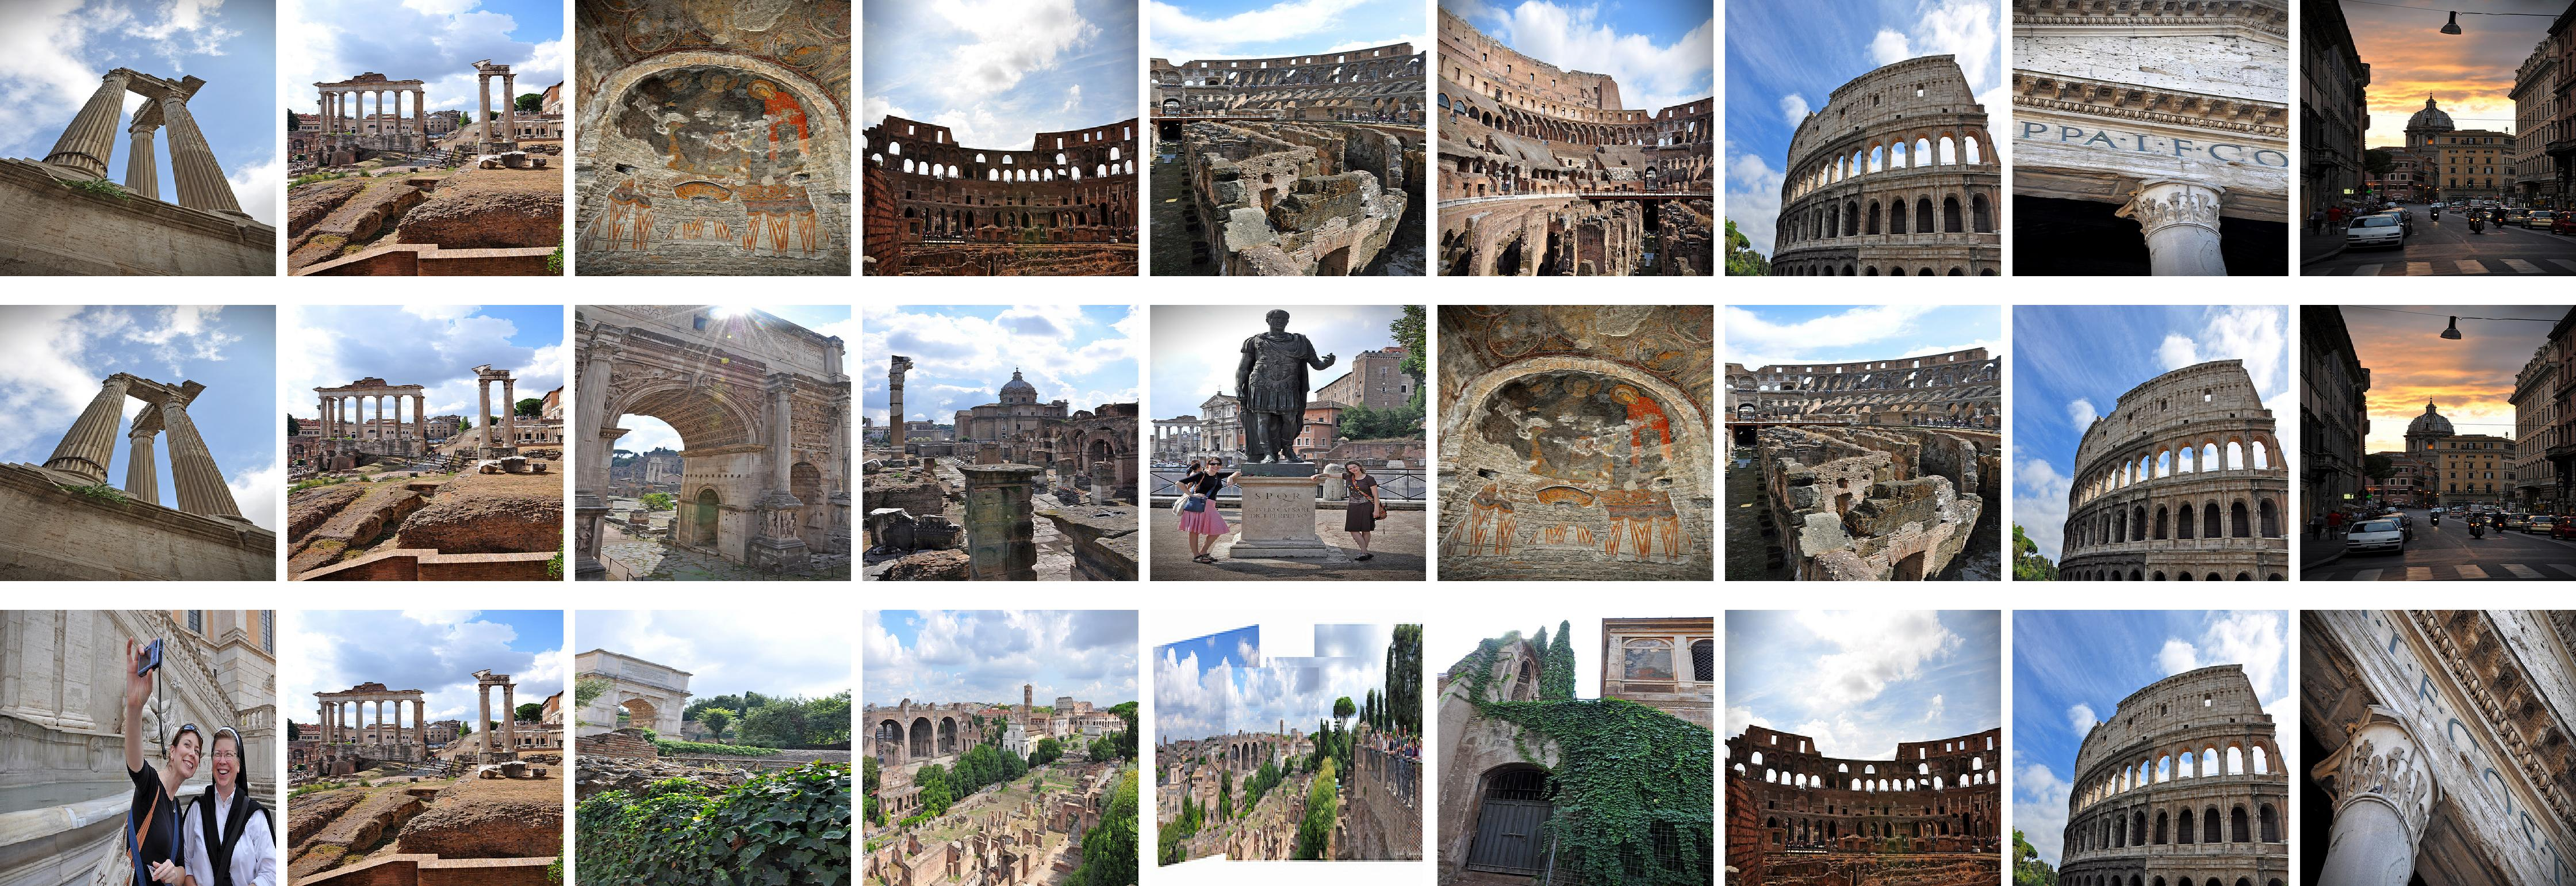
\includegraphics[height=1.5in]{results/b9_3_12515159@N07_9_20.jpg}}
     \subcaptionbox{Top 20\% of a \textit{Wedding} album. \label{fig46}}{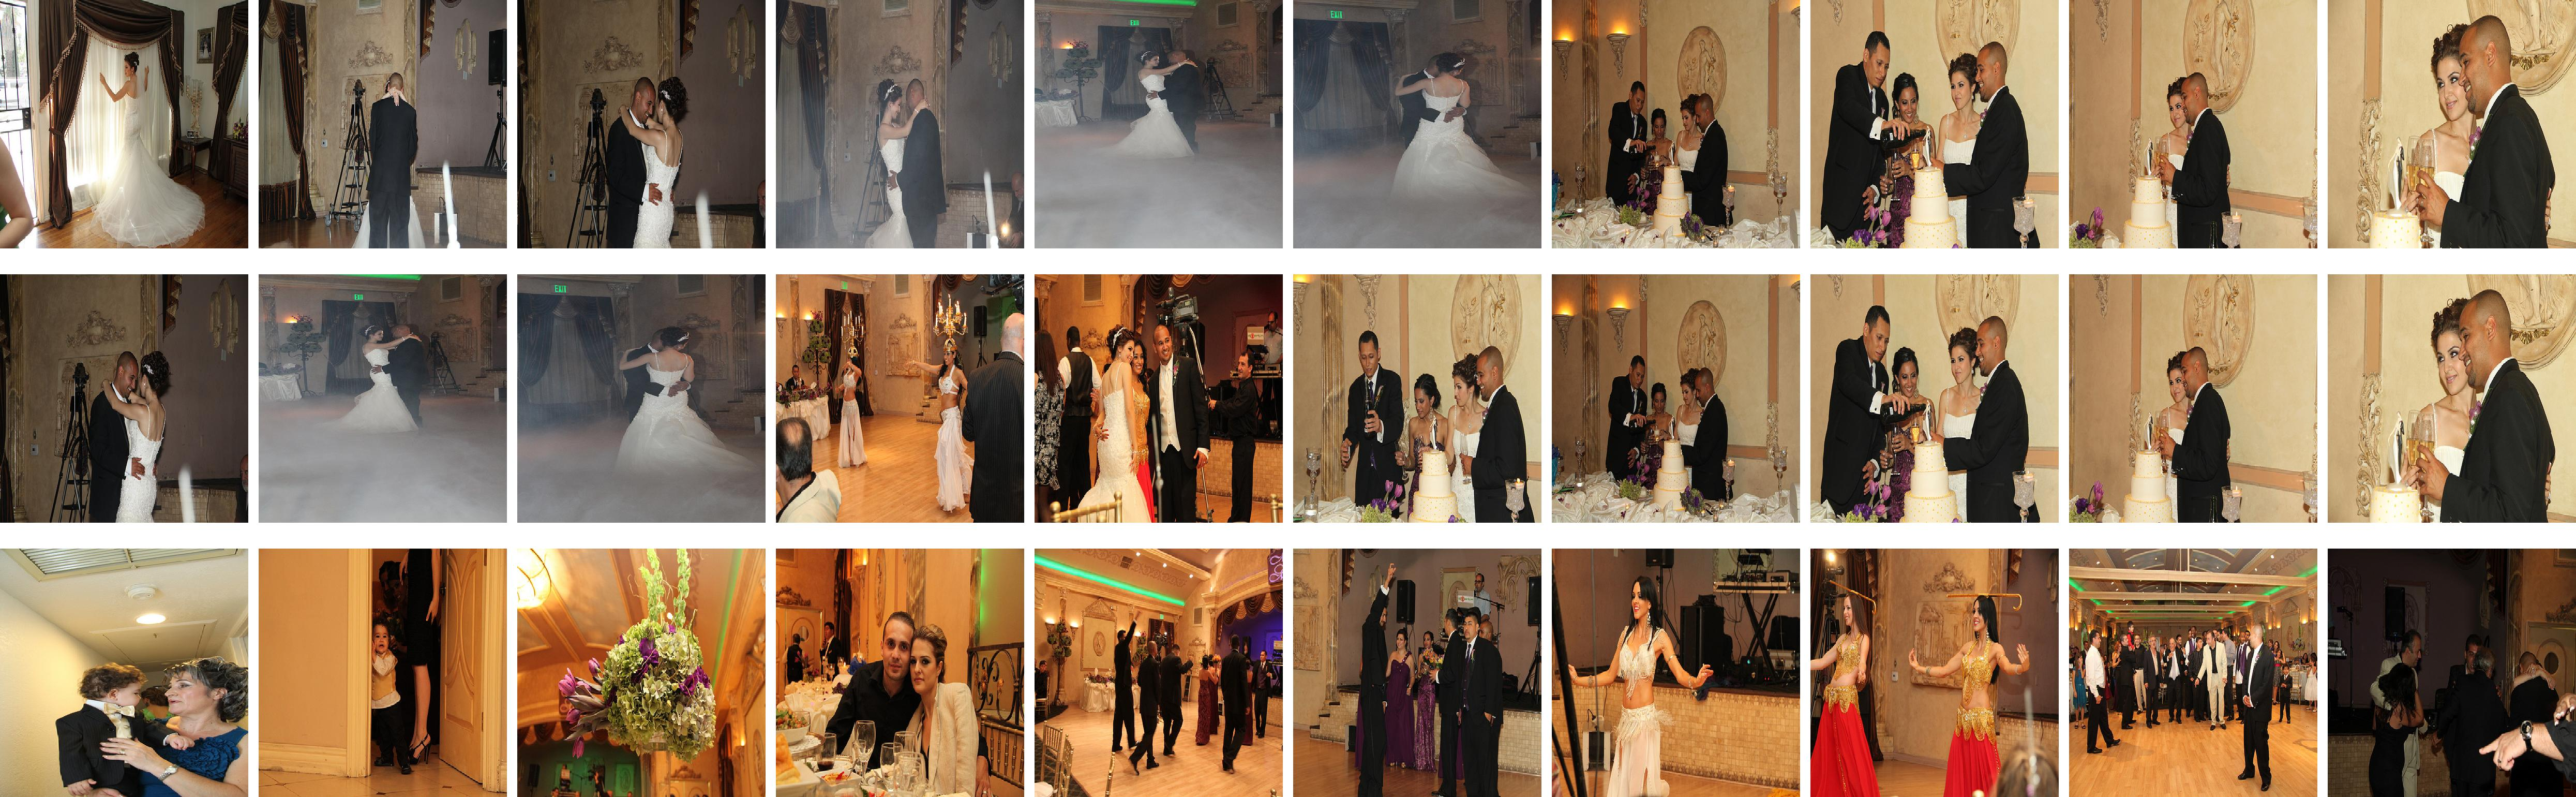
\includegraphics[height=1.5in]{results/b10_5_12482312@N00_10_20.jpg}}
     \subcaptionbox{Top 20\% of a \textit{Zoo} album. \label{fig47}}{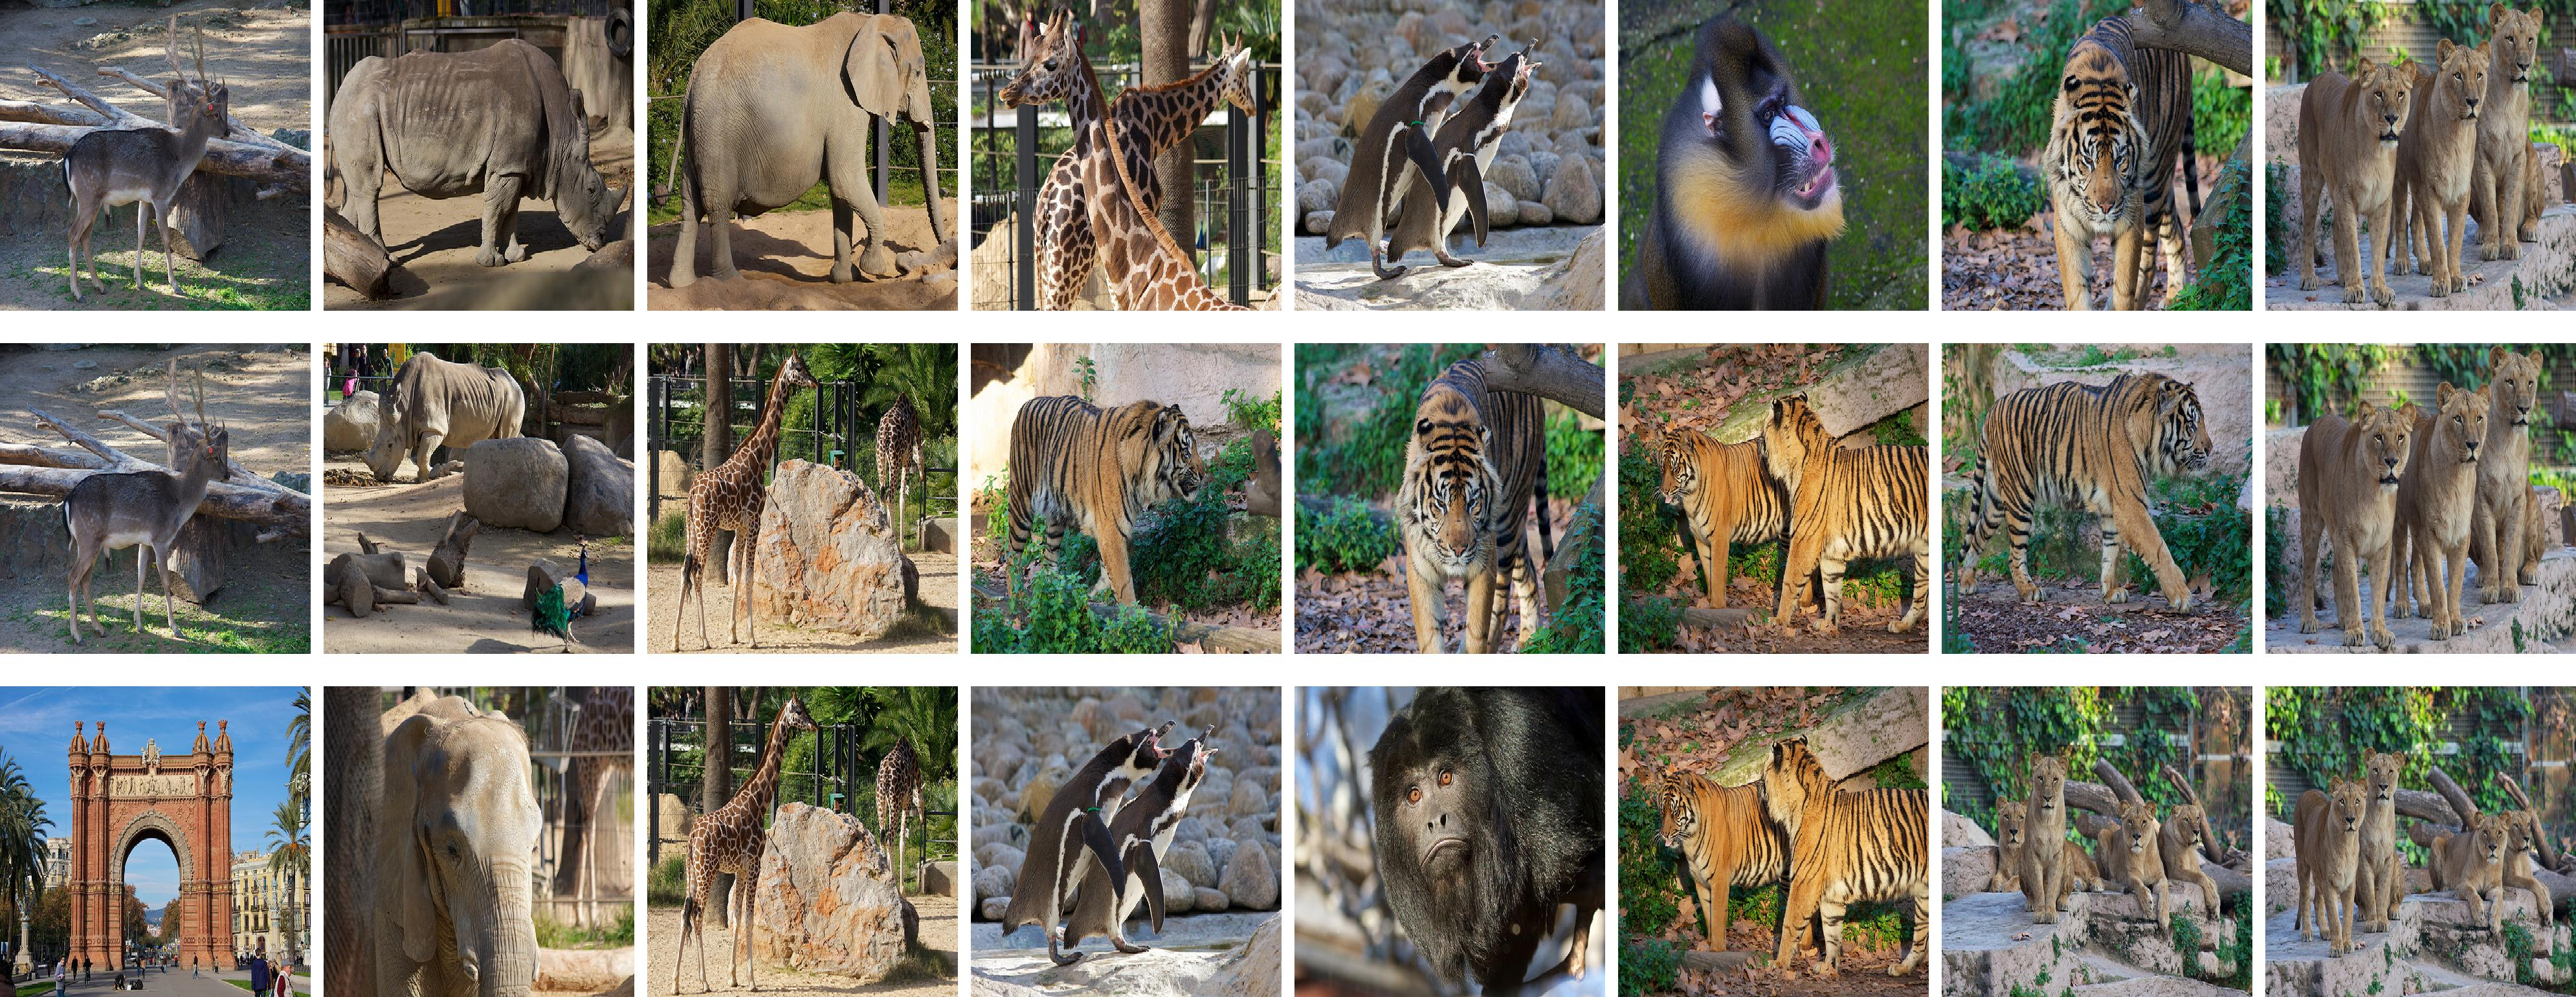
\includegraphics[height=1.5in]{results/b11_5_25093253@N05_8_20.jpg}}    
     \end{figure*}
        
  \clearpage
  \begin{figure*}[ht]
  \ContinuedFloat % continue from previous page
\centering
     \subcaptionbox{Top 10\% of a \textit{Graduation} album. \label{fig48}}{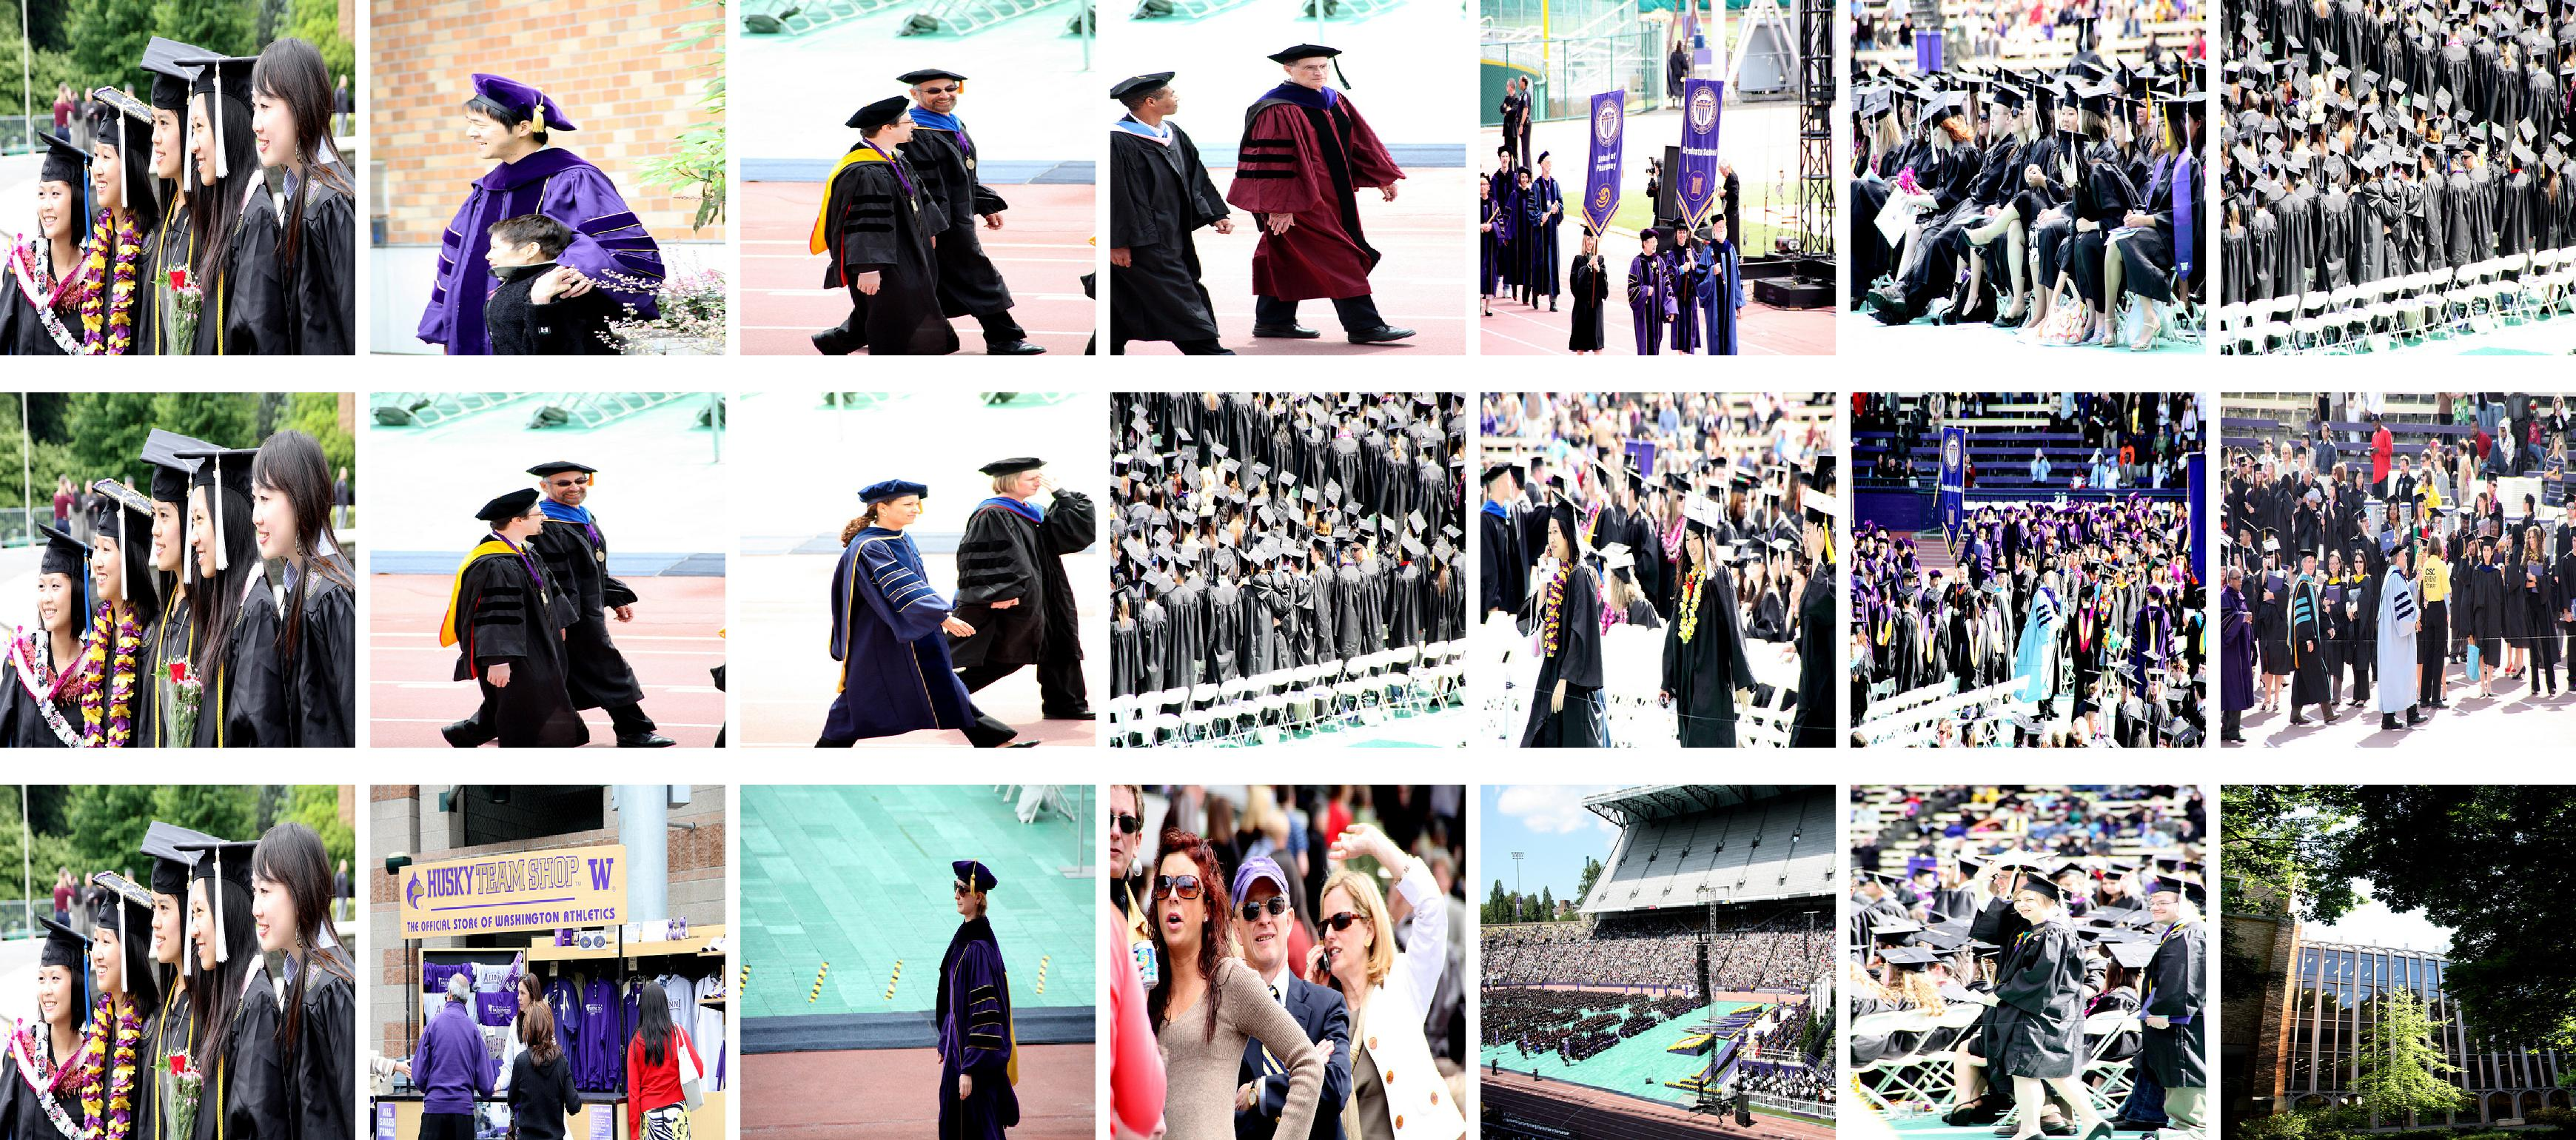
\includegraphics[height=1.5in]{results/b12_5_25369032@N00_7_10.jpg}}
     \subcaptionbox{Top 20\% of a \textit{Museum} album. \label{fig49}}{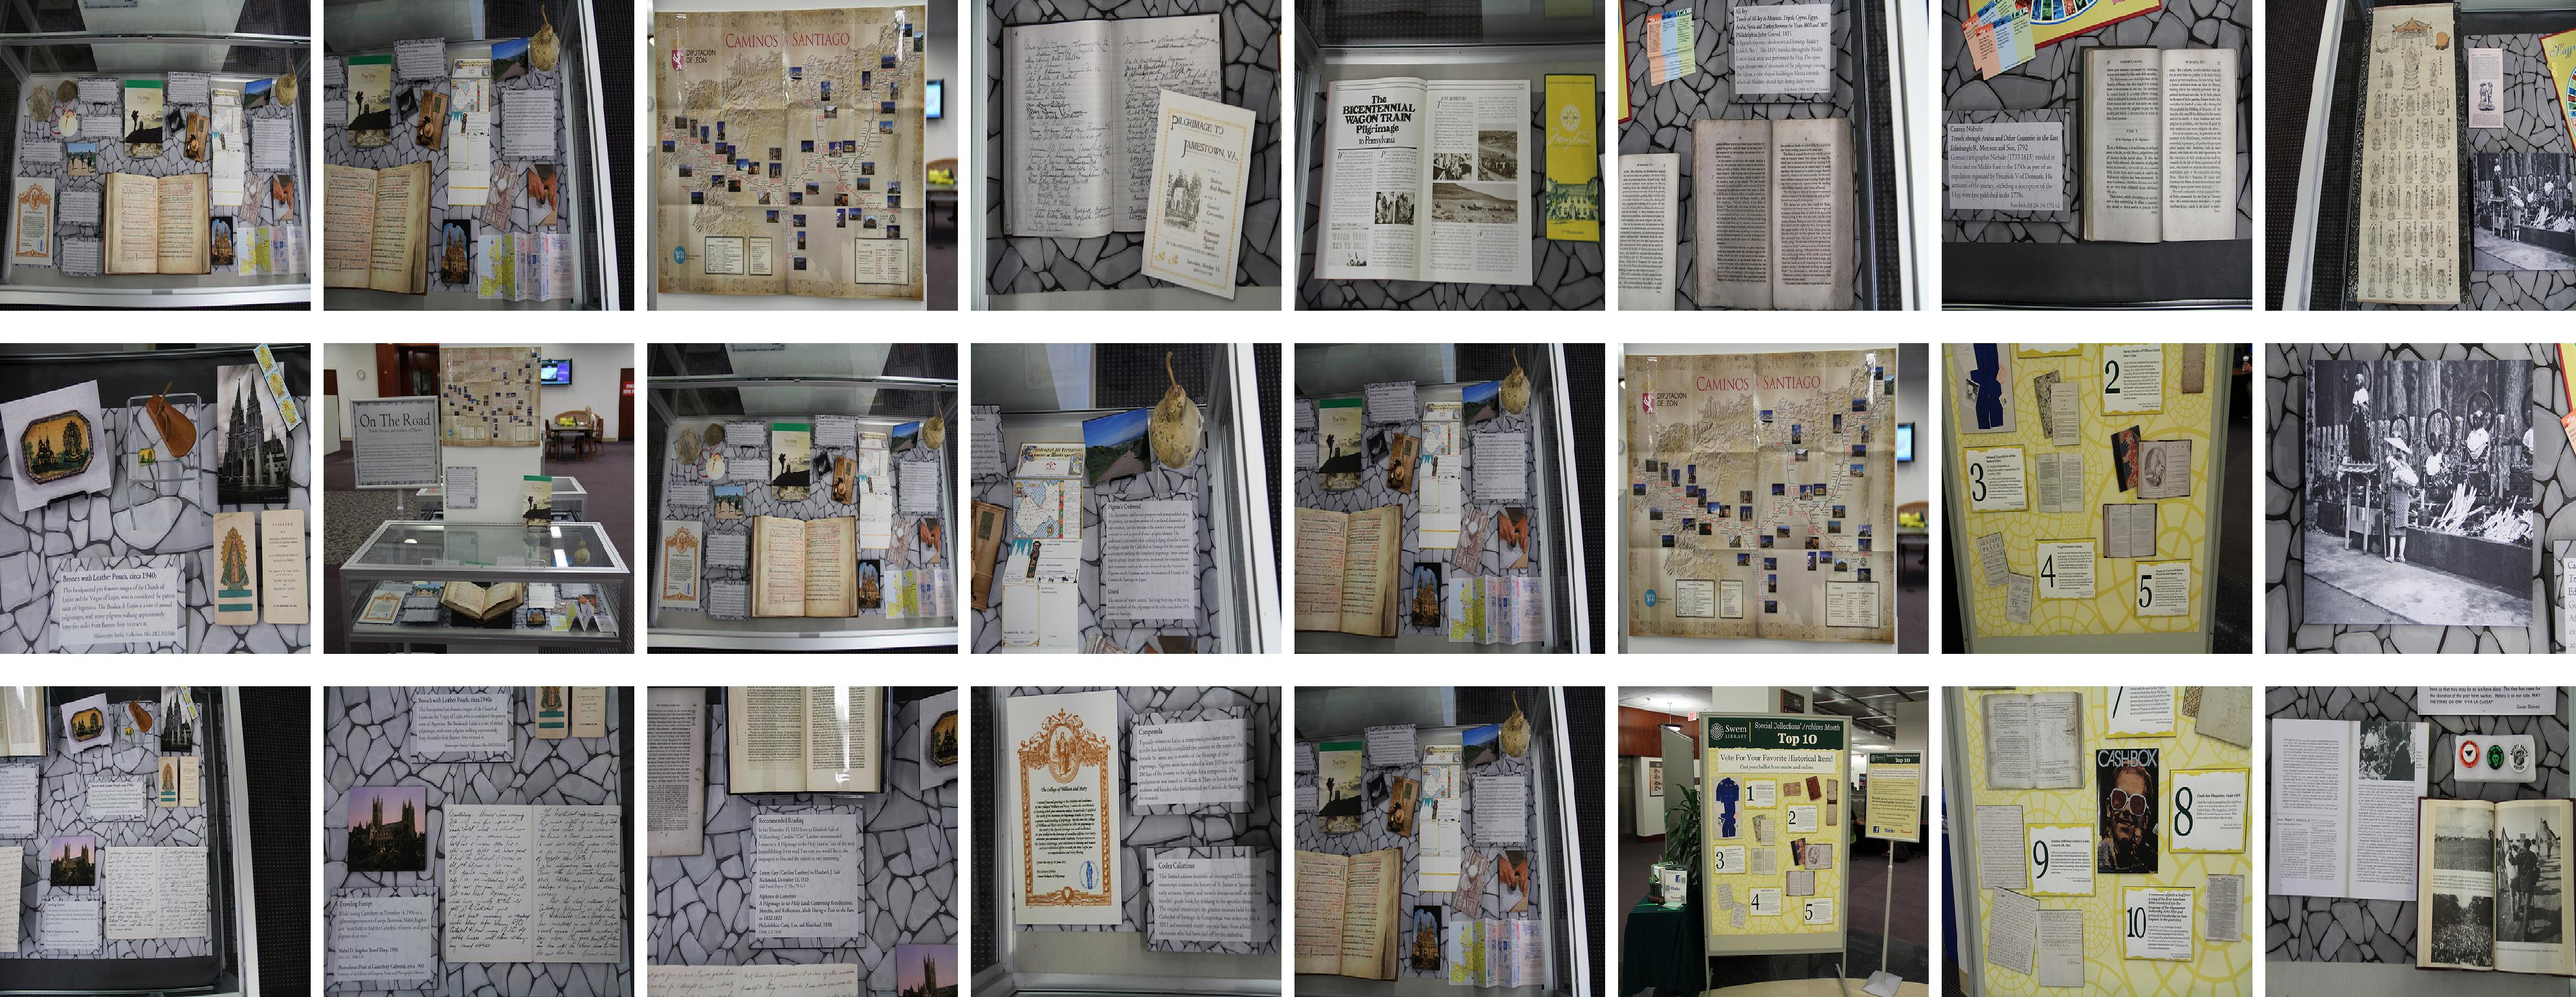
\includegraphics[height=1.5in]{results/b13_7_7349747@N02_8_20.jpg}}
     \subcaptionbox{Top 20\% of a \textit{Beach Trip} album. \label{fig50}}{\includegraphics[height=1.5in]{results/b14_7_47519867@N07_7_20.jpg}} \\
     \subcaptionbox{Top 10\% of a \textit{Nature Trip} album. \label{fig51}}{\includegraphics[height=1.5in]{results/b15_7_69966484@N00_7_10.jpg}}
     \subcaptionbox{Top 10\% of a \textit{Zoo} album. \label{fig52}}{\includegraphics[height=1.5in]{results/b16_8_43257106@N07_8_10.jpg}}
           \end{figure*}
        
  \clearpage
  \begin{figure*}[ht]
  \ContinuedFloat % continue from previous page
\centering
     \subcaptionbox{Top 20\% of a \textit{Zoo} album. \label{fig53}}{\includegraphics[height=1.5in]{results/b17_8_66724483@N00_6_20.jpg}}
     \subcaptionbox{Top 15\% of a \textit{Zoo} album. \label{fig54}}{\includegraphics[height=1.5in]{results/b18_8_84905000@N00_10_15.jpg}}
     \subcaptionbox{Top 10\% of a \textit{Zoo} album. \label{fig55}}{\includegraphics[height=1.5in]{results/b19_25_90514086@N00_9_10.jpg}}
     \subcaptionbox{Top 15\% of a \textit{Protest} album. \label{fig56}}{\includegraphics[height=1.5in]{results/b20_9_28657663@N00_10_15.jpg}}
     \subcaptionbox{Top 20\% of a \textit{Wedding} album. \label{fig57}}{\includegraphics[height=1.5in]{results/b21_13_44564547@N00_7_20.jpg}} \hspace{2em}
     \subcaptionbox{Top 20\% of a \textit{Christmas} album. \label{fig58}}{\includegraphics[height=1.5in]{results/b22_14_53746192@N00_6_20.jpg}}
       \caption{Example of results. For each album, top 10-20\% images of the album from three methods are shown. Images are arranged in chronological order. First row is the ground truth we acquired from AMT workers; second row is our prediction using Ensemble-CNN which we introduced in the main paper; third row is the result from random selection.}
         \end{figure*}
         
         
  \clearpage
  \begin{figure*}[ht]
\centering
  \subcaptionbox{Top 20\% of a \textit{Museum} album. \label{fig59}}{\includegraphics[height=1.5in]{results/c1_14_97402086@N00_6_20.jpg}} \\
  \subcaptionbox{Top 15\% of a \textit{Birthday} album. \label{fig60}}{\includegraphics[height=1.5in]{results/c2_24_97863854@N00_8_15.jpg}}
    \subcaptionbox{Top 20\% of a \textit{Personal Sports} album. \label{fig61}}{\includegraphics[height=1.5in]{results/c3_20_9674366@N08_8_20.jpg}} 
  \subcaptionbox{Top 20\% of a \textit{Show} album. \label{fig62}}{\includegraphics[height=1.5in]{results/c4_38_27988337@N00_10_20.jpg}}
  \subcaptionbox{Top 15\% of a \textit{Theme Park} album. \label{fig63}}{\includegraphics[height=1.5in]{results/c5_18_97864553@N00_9_15.jpg}}
           \end{figure*}
         
         
  \clearpage
  \begin{figure*}[ht]
    \ContinuedFloat % continue from previous page
\centering
      \subcaptionbox{Top 20\% of a \textit{Sports} album. \label{fig64}}{\includegraphics[height=1.5in]{results/c6_35_59755673@N04_6_20.jpg}} \\
    \subcaptionbox{Top 20\% of a \textit{Wedding} album. \label{fig65}}{\includegraphics[height=1.5in]{results/c7_49_30952578@N00_6_20.jpg}} \\
    \subcaptionbox{Top 10\% of a \textit{Museum} album. \label{fig66}}{\includegraphics[height=1.5in]{results/c8_17_16036153@N04_8_10.jpg}}
    \subcaptionbox{Top 15\% of a \textit{Nature Trip} album. \label{fig67}}{\includegraphics[height=1.5in]{results/c9_41_22539273@N00_9_15.jpg}}
    \subcaptionbox{Top 20\% of a \textit{Theme Park} album. \label{fig68}}{\includegraphics[height=1.5in]{results/c10_50_12734746@N00_10_20.jpg}}
   \end{figure*}
         
  \clearpage
  \begin{figure*}[ht]
    \ContinuedFloat % continue from previous page
\centering 
    \subcaptionbox{Top 20\% of a \textit{Theme Park} album. \label{fig69}}{\includegraphics[height=1.5in]{results/c11_51_66478195@N00_7_20.jpg}} \hspace{2em}
    \subcaptionbox{Top 20\% of a \textit{Casual Family/Friends Gathering} album. \label{fig70}}{\includegraphics[height=1.5in]{results/c12_78_14451269@N00_6_20.jpg}}
    \subcaptionbox{Top 20\% of a \textit{Personal Art Activity} album. \label{fig71}}{\includegraphics[height=1.5in]{results/c13_85_43162195@N00_8_20.jpg}}
    \subcaptionbox{Top 15\% of a \textit{Theme Park} album. \label{fig72}}{\includegraphics[height=1.5in]{results/c14_95_66478195@N00_9_15.jpg}}
    \subcaptionbox{Top 20\% of a \textit{Personal Art Activity} album. \label{fig73}}{\includegraphics[height=1.5in]{results/c15_124_8798099@N02_8_20.jpg}}
    \subcaptionbox{Top 20\% of a \textit{Zoo} album. \label{fig74}}{\includegraphics[height=1.5in]{results/c16_155_27998473@N02_9_20.jpg}}
           \caption{Example of results. For each album, top 10-20\% images of the album from three methods are shown. Images are arranged in chronological order. First row is the ground truth we acquired from AMT workers; second row is our prediction using Ensemble-CNN which we introduced in the main paper; third row is the result from random selection.}
         \end{figure*}

  
{\small
\bibliographystyle{ieee}
\bibliography{egbib}
}

\end{document}